\documentclass[10pt,openany]{book}

\usepackage[T1]{fontenc}
\usepackage[utf8]{inputenc}
\usepackage[english]{babel}
\usepackage{geometry}
\usepackage{graphicx}
\usepackage[pdfa=true]{hyperref}
\usepackage{cite}
\usepackage{listings}
\usepackage[printonlyused,withpage]{acronym}
\usepackage{siunitx}
\usepackage{multirow}
\usepackage{setspace}
\usepackage{xcolor}
\usepackage{array}
\usepackage{listings}
\usepackage{tabularx}
\usepackage{marvosym}
\usepackage{amsmath}
\usepackage{amssymb}
\usepackage[noend]{algpseudocode}
\usepackage{algorithmicx,algorithm}

%--- pdf/a format ----
% insert metadata about the document here
\RequirePackage{filecontents}
\begin{filecontents*}{\jobname.xmpdata}
\Title{Document’s title}
\Author{Author’s name}
\Language{en-US}
\Subject{The abstract, or short description.}
\Keywords{keyword1\sep keyword2\sep keyword3}
\end{filecontents*}
\usepackage{colorprofiles}
\usepackage[a-1b,mathxmp]{pdfx}[2018/12/22]
\usepackage[T1]{fontenc}
\hypersetup{pdfstartview=}


%
% This is the official thesis template of
% the Institute of Computer Science at the
% Georg-August-University of Göttingen
%
%      author: kellner@cs.uni-goettingen.de
% last update: 17/02/2015
%
% If you find any sort of mistake please let me know
% so that it can be fixed in future releases.
%


%--- include custom commands ---
%
% own commands
%

%double empty page
\newcommand \myemptypage {
    \clearpage
    \thispagestyle{empty}
    \null
    \cleardoublepage
}

%create abstract environment that is not available in latex book style
\newcommand\abstractname{Abstract}
\newenvironment{abstract}{%
    \begin{center}%
        \normalfont\Large\bfseries \abstractname
    \end{center}%
    \it%
    }
    {}


%--- include general configuration ---
%
% general configuration
%

% Palatino font as serif font
\usepackage{palatino}
\linespread{1.05}
% Helvatica font as sans-serif
\usepackage{helvet}
% Use microtype to improve typesetting
\usepackage{microtype}

%set page margin for DIN A4
\geometry{a4paper, left=2.5cm, right=2.5cm, top=4cm, 
          bottom=5cm, bindingoffset=1cm}

%makes TeX less fussy about line breaking
\sloppy

% Replacement for changing parskip and parindent directly
\usepackage{parskip}

%1.5 spacing
\onehalfspacing
{}

% Make chapter heading smaller
\usepackage{titlesec}
\titleformat{\chapter}[display]
  {\LARGE\bf}{\chaptertitlename\ \thechapter}{10pt}{\huge\bf}

%define some colors
\definecolor{darkblue}{rgb}{0.0,0.0,0.5}
\definecolor{grey}{rgb}{0.8,0.8,0.8}
\definecolor{lightgrey}{rgb}{0.95,0.95,0.95}

%set listing style properties for python
\lstset{language=Python,
    basicstyle=\footnotesize\ttfamily,
    captionpos=b,
    frame=tb,
    commentstyle=\color{gray} \bfseries,
    stringstyle=\color{green}\ttfamily,
    keywordstyle=\color{darkblue}\bfseries,
    breaklines=true,
    aboveskip=10mm,
    belowskip=10mm,
    showstringspaces=false
    numbers=left,
    %stepnumber=5,
    numberstyle=\tiny,
    numbersep=5pt
}


%override reference title and listings title
\renewcommand \bibname{References}
\renewcommand{\lstlistlistingname}{List of Listings}




%--- basic document configuration ---
\newcommand{\mytype}{Bachelor's Thesis}
%\newcommand{\mytype}{Master's Thesis}

\newcommand{\mycourse}{Applied Computer Science}
%\newcommand{\mycourse}{Internet Technologies and Information Systems}

\newcommand{\mytitle}{Data Classification in Medical/Healthcare: Classification Methods Comparison under Class Imbalance}
\newcommand{\myauthor}{Mengru Ji}
\newcommand{\mydepartment}{Institute of Computer Science}
\newcommand{\mysubmissiondate}{13. March 2021}
\newcommand{\mythesisid}{201x-xx} %assigned by examination office
\newcommand{\myfirstsupervisor}{Prof. Dr. Xiaoming Fu}
\newcommand{\mysecondsupervisor}{Dr. Tingting Yuan}


\begin{document}

    \pagenumbering{roman}
    \setcounter{page}{1}

   %--- cover page ---
    %
% title page
%

\begin{titlepage}
    %--- logo ---
    \normalsize
    \begin{tabularx}{\textwidth}{lXr}
        \multirow{2}{*}{
\includegraphics[width=6.5cm]{images/goe-logo.jpg}} 
        & & ISSN 1612-6793\\
    \end{tabularx}

    %default settings for the rest
    \large
    \centering

    \vspace{3cm}

    \textbf{\LARGE \mytype}\\

    submitted in partial fulfillment of the\\
    requirements for the course ``\mycourse''

    \vspace{2cm}

    \textbf{\LARGE \mytitle}

    \vspace{2cm}

    \myauthor

    \vspace{2cm}

    \mydepartment

    \vspace{2cm}

    Bachelor's and Master's Theses\\
    of the Center for Computational Sciences\\
    at the Georg-August-Universität Göttingen

    \vspace{0.2cm}

    \mysubmissiondate


    %--- new page ---
    %\myemptypage
    \clearpage
    \thispagestyle{empty}
    \null
    \flushleft
    \onehalfspacing
    \normalsize

    \vspace{12cm}

    Georg-August-Universität Göttingen\\
    Institute of Computer Science\\[3ex]
    Goldschmidtstraße 7\\
    37077 Göttingen\\
    Germany\\[3ex]

    \begin{tabular}{@{}ll}
        \Telefon & +49 (551) 39-172000\\
        \fax & +49 (551) 39-14403\\
        \Letter & \href{mailto:office@informatik.uni-goettingen.de}{office@informatik.uni-goettingen.de}\\
        \Mundus & \url{www.informatik.uni-goettingen.de}\\
    \end{tabular}

    \vspace{1.0cm}

    \begin{tabular}{@{}ll}
        First Supervisor: & \myfirstsupervisor\\
        Second Supervisor:& \mysecondsupervisor\\
    \end{tabular}

    \clearpage
\end{titlepage}


    %\myemptypage

    %--- statement page ---
    \thispagestyle{empty}

\null
\vspace{16.5cm}

\rule{\textwidth}{0.4pt}

I hereby declare that I have written this thesis independently without any help from others and without the use of documents or aids other than those stated. I have mentioned all used sources and cited them correctly according to established academic citation rules.

\vspace{0.2cm}

Göttingen, \mysubmissiondate

    %\myemptypage

    %--- abstract ---
    \clearpage\phantomsection\pdfbookmark{\abstractname}{abstract}
    \thispagestyle{empty}
    \begin{abstract}
Recently, machine learning has become a popular topic in the computer field and classification is one of the most prevalent directions in machine learning. There are many standard and commonly used classification methods, such as Na{\"i}ve Bayes, k-nearest neighbor (kNN), support vector machine and decision tree. Most classification algorithms assume that the dataset is balanced distributed, but data obtained from real life can hardly meet this prerequisite. In the real world, the impact of data imbalance in many domains is pervasive, such as in fraud detection, risk management, text classification and medical diagnosis. Especially in the medical or healthcare sector, the cost of missing a patient is much more expensive than that of classifying a healthy person as a patient. If this problem is ignored, it will not be easy to guarantee the accuracy of the classification task.

Due to the prevalence of class imbalance problem in medical or healthcare sector, in order to have a comprehensive and deep understanding of the imbalance classification algorithms, in this paper, a comparison of the binary classification performance of several classical and state-of-the-art class imbalance classification algorithms was carried out on several datasets. The data used for the experiments was taken from UCI, KEEL and OpenML which included not only the data from the medical/healthcare sector but also some other widely used datasets.

The algorithms used for the comparison included DDAE, MWMOTE, SMOTE, RUSBoost, AdaBoost, cost-sensitive decision tree (csDCT), self-paced Ensemble Classifier, MetaCost, CAdaMEC and Iterative Metric Learning (IML), most of which come from three main groups of class imbalance classification, namely sampling, cost-sensitive learning and ensemble learning. The experiments mainly focused on an overall comparison, the impact of imbalance ratio and the size of the given dataset on the performance of the above-mentioned algorithms. Mainly DDAE is researched, including the effectiveness of each component and the impact of parameters upon it. Sampling methods are not suitable all the time since they need to consider the neighborhoods based on distance. However, some classifiers can be improved after the balance of class distribution. Cost-sensitive learning models should be utilized when the dataset is less in imbalance, because it is difficult to set an appropriate cost matrix for the specific dataset, which can cause the fluctuations of their performances. Ensemble learning techniques perform better as they approach the problem from many angles, but they absorb not only the advantages but also the disadvantages of the techniques used. In addition, according to the results, the Data Block Construction (DBC) was the most important component in DDAE. Also, its parameter tuning process showed as the most appropriate parameter for the model, especially in the experiment on the number of data blocks of DDAE, which illustrates the impact of the number of base learners on the performance of ensemble learning algorithms.

\end{abstract}


    %\myemptypage
    
    %-- acknowledgement
    \chapter*{Acknowledgements}
    \pdfbookmark[1]{Acknowledgements}{acknowledgements}
    %\begin{acknowledgement}
Here, I would like to sincerely acknowledge individuals who have supported me directly or indirectly for the accomplishment of this paper.

First of all, I would like to express my sincere gratitude to my first supervisor Prof. Dr. Xiaoming Fu for his helpful suggestions for me and for my paper. Secondly, I would like to thank Dr. Tingting Yuan for being my second supervisor and guiding me with her comments.  Next,  I would like  to specially thank Mr. Yachao Shao, who has been my advisor throughout the journey towards completion of my paper. I would like to thank him for his constant encouragement, guidance and tireless assistance. Without their usual and enlightening guidance, this paper would not have been in its present form.

I would like to thank my dear family for their love and great faith in me for many years, even though they cannot be beside me. I also want to thank my dear friends and my roommate, who have given me help and time to listen to my opinions and comforted me when I felt upset or faced difficulties. While it would be difficult to list all their names, I would like to express my gratitude to each of my family members and friends in China and in Germany. Without their support and help, the completion of this paper would not have been possible.

Finally, I would like to thank the faculty of Computer Science of the Georg-August University of G{\"o}ttingen. I would like to thank all the staff members of the department who have provided me with information required and answered my questions with patience.

%\end{acknowledgement}

    
    %reset acronyms after abstract
    \acresetall

    %--- table of contents ---
    \clearpage\phantomsection\pdfbookmark{\contentsname}{toc}
    \tableofcontents
  %  \myemptypage

    %--- list of figures ---
    \listoffigures
  %  \myemptypage

    %--- list of tables ---
    \listoftables
    \thispagestyle{empty}
    \myemptypage

    %--- list of listings ---
    %\lstlistoflistings
    %\myemptypage

    %--- list of acronyms ---
    %\chapter*{List of Abbreviations}

\begin{acronym}[myacronyms]
    \acro{FYI}{For Your Information}    
\end{acronym}

    %\myemptypage


    %arabic page numbers
    \pagenumbering{arabic}
    \setcounter{page}{1}
    
    %--- chaper 1..n ---
    \chapter{Introduction}

\section{Background}
In recent times, machine learning has advanced briskly and has become an attractive research topic in the domain of computer science. The classification problem is one of the most prevalent directions of machine learning \cite{11}, and many researchers have paid attention to binary imbalance classification \cite{90}. There are many standard and commonly used classification methods that are already known, such as C4.5 \cite{103}, support vector machine \cite{92}, k-nearest neighbor(kNN) \cite{75} and random forest \cite{39}. Most algorithms used for classification consider the datasets are to be balanced distributed, but data obtained from real life can hardly meet this prerequisite \cite{47}. The class imbalance of the data will impact on the performance of almost all standard classification algorithms \cite{11}. Since the number of instances of one class is more than that of another class, the model is likely to be confused by the majority during the learning process so that it does not perform well in the final classification of the test data \cite{17}. In the real world, the impact of data imbalance in many fields is pervasive, such as medical diagnosis, fraud detection and text classification \cite{47}. This is especially true in the medical or healthcare field, because patients with a particular disease themselves belong to a minority in society and because of the complexity of medical information, the process of collecting information is prone to record errors or data omissions \cite{5,7}. If this problem is ignored, it will not be easy to guarantee accuracy when using classification algorithms to predict testing data \cite{17}. This is not only a waste of resources, but it can also lead to misdiagnosis due to incorrect predictions, which will endanger the lives of patients in severe cases \cite{18,21}. Therefore, this problem has critical importance and its probability of occurrence is very high. 

According to previous research, the imbalance problem of classes can be improved mainly in the following areas: (1) Sampling technique \cite{9}: including oversampling and undersampling; (2) Cost-sensitive learning \cite{19}: where the value of the majority class is often different from that of the minority class which also shows that the cost of predicted minority samples as the majority sample is more expensive than that of predicted majority sample as the minority sample \cite{18}; and, (3) Ensemble learning \cite{33} inspired by the popular saying that the minority obeys the majority, that is, Major Voting. A certain number of basic classifiers will be used to predict all anonymous data samples, and then the final label of a particular sample will be determined according to the number of votes \cite{26}. 

In the past two decades, assorted models have been developed to address the problem of class imbalanced classification. Most of them are the application of the three ideas mentioned in the previous paragraph or a combination of them. For example, the SMOTE \cite{13}  belonging to the field of resampling, the Adacost \cite{94} algorithm utilizing both cost-sensitive learning and the ensemble learning technique, and the application of ensemble learning in RUSBoost \cite{64}. These are classical algorithms in the field of imbalanced learning, and have been applied to process data from multiple fields. In addition, there are many algorithms that focus on data imbalance in the medical and health fields, such as \cite{3,5,8}.

Due to the variety of imbalance classification algorithms, it can be hard to see the differences between them. To understand them better, this paper focuses on comparing the performance of different types of imbalance classification algorithms on multiple datasets which are not only from medical/healthcare sector but also from other popular fields. There are seven classical imbalanced classification algorithms, including (1) sampling: SMOTE \cite{13} and MWMOTE \cite{62}; (2) cost-sensitive learning: MetaCost \cite{23}, CAdaMEC \cite{67} and cost-sensitive decision tree \cite{10}; and (3) ensemble learning: AdaBoost \cite{63} and RUSBoost \cite{64}, with three newer state-of-art models, namely DDAE \cite{73}, Iterative Metric Learning(IML) \cite{72} and self-paced Ensemble Classifier \cite{96}, developed in recent years and selected as a comparison. The experiment first analyzes the performance of different models based on their evaluation metrics on the same dataset. Secondly, the impact of other factors, such as the size of the dataset and the imbalance ratio, are illustrated. In the final part of the experiment, the importance of the various components of DDAE is presented.

\section{Outline of Thesis}
This paper is structured as follows. The background and objective are presented in Chapter 1. Chapter 2 focuses on the previous works on the class imbalance problem and some of the classification methods applied in the medical/healthcare sector. In Chapter 3, the methodology containing detail about the implementation DDAE model and IML model is described. Chapter 4 shows input data and presents the result of experiment. The overall results are discussed and concluded in Chapter 5.




% \newpage

% This is the introduction chapter that shows the basic use of some latex commands that can be used in the document. Of course there is a lot more in latex that cannot be covered here.


% \section{Document Structure}
% The document structure is defined by the \texttt{documentclass} command in the main latex file. Here the \texttt{book} format is used that supports the following subdivisions:

% \texttt{\textbackslash chapter} -- A book chapter\\
% \texttt{\textbackslash section} -- A section in a chapter\\
% \texttt{\textbackslash subsection} -- A subsection in a section of a chapter\\
% \texttt{\textbackslash subsubsection} -- A subsubsection in a subsection of section in a chapter\\

% Each of the subdivisions is automatically numbered. If the numbering should be omitted, add a \texttt{*} to the command e.g.:
% \begin{verbatim}
%     \section*{My Section}
% \end{verbatim}

% Additionally, paragraphs can be defined:
% \texttt{\textbackslash paragraph} -- A paragraph\\
% \texttt{\textbackslash subparagraph} -- A subparagraph in a paragraph\\



% \section{Paragraph Formatting}

% Paragraphs can be aligned in different ways:

% \begin{flushleft}
%     You can flush a paragraph to the left that is the default.
% \end{flushleft}
% \begin{verbatim}
% \begin{flushleft}
%     You can flush a paragraph to the left that is the default.
% \end{flushleft}
% \end{verbatim}

% \begin{flushright}
%     Or you can flush a paragraph to the right.
% \end{flushright}
% \begin{verbatim}
% \begin{flushright}
%     Or you can flush a paragraph to the right.
% \end{flushright}
% \end{verbatim}

% \begin{center}
%     Or you can center the paragraph.
% \end{center}
% \begin{verbatim}
% \begin{center}
%     Or you can center the paragraph.
% \end{center}
% \end{verbatim}

% There is also the \texttt{verbatim} paragraph that does not interpret the text. This can be used, for example, to show some source code. However, for an improved source code handling see the \texttt{lstlisting} package.
% \begin{verbatim}
% #include<stdio.h>

% int main() {
%     printf("Hello World\n");

%     return 0;
% }
% \end{verbatim}

% \section{Font}

% \subsection{Emphasizing}
% Text can be \emph{emphasized} as follows:
% \begin{verbatim}
% \emph{emphasized text}
% \end{verbatim}

% To emphasize a word \textbf{more heavily} do:
% \begin{verbatim}
% \textbf{bold text}
% \end{verbatim}

% \subsection{Font Styles}
% There are different options to style a font. The most important are:

% Use the \textsf{sans serif font family}:
% \begin{verbatim}
% \textsf{sans serif font family}
% \end{verbatim}

% Use the \texttt{teletypefont family} (monospace font):
% \begin{verbatim}
% \texttt{teletypefont family}
% \end{verbatim}


% \subsection{Font Sizes}

% Be aware of the different font sizes:

% {\tiny \texttt{\textbackslash tiny}}\\
% {\scriptsize \texttt{\textbackslash scriptsize}}\\
% {\footnotesize \texttt{\textbackslash footnotesize}}\\
% {\small \texttt{\textbackslash small}}\\
% {\normalsize \texttt{\textbackslash normalsize}}\\
% {\large \texttt{\textbackslash large}}\\
% {\Large \texttt{\textbackslash Large}}\\
% {\LARGE \texttt{\textbackslash LARGE}}\\
% {\huge \texttt{\textbackslash huge}}\\
% {\Huge \texttt{\textbackslash Huge}}\\


% \section{Colors}
% The \texttt{xcolor} package allows to set the font color. The easiest way to change the \textcolor{red}{red} of a text is to use:
% \begin{verbatim}
% \textcolor{red}{red text}
% \end{verbatim}
% There are a couple of pre-defined color names available, but of course custom colors can be defined as well. See the \texttt{xcolor} package manual for details.


% \section{List Structures}
% There are different ways to define a list in latex:

% As unordered list:
% \begin{itemize}
%     \item One
%     \item Two
%     \item Three
% \end{itemize}
% \begin{verbatim}
% \begin{itemize}
%     \item One
%     \item Two
%     \item Three
% \end{itemize}
% \end{verbatim}


% Or as ordered list:
% \begin{enumerate}
%     \item One
%     \item Two
%     \item Three
% \end{enumerate}
% \begin{verbatim}
% \begin{enumerate}
%     \item One
%     \item Two
%     \item Three
% \end{enumerate}
% \end{verbatim}


% Or as description list:
% \begin{description}
%     \item[First] One
%     \item[Second] Two
%     \item[Third] Three
% \end{description}
% \begin{verbatim}
% \begin{description}
%     \item[First] One
%     \item[Second] Two
%     \item[Third] Three
% \end{description}
% \end{verbatim}

% Of course lists can also be nested:
% \begin{enumerate}
%     \item One
%         \begin{enumerate}
%             \item alpha
%             \item beta
%         \end{enumerate}
%     \item Two
%     \item Three
% \end{enumerate}
% \begin{verbatim}
% \begin{enumerate}
%     \item One
%         \begin{enumerate}
%             \item alpha
%             \item beta
%         \end{enumerate}
%     \item Two
%     \item Three
% \end{enumerate}
% \end{verbatim}


% \section{Tables}

% The \texttt{tabular} environment can be used to create a simple table:
% \begin{tabular}{l|c|p{3cm}|r}
%     1 & 2 & 3 & 4 \\
%     5 & 6 & 7 & 8\\[6pt]
%     \hline
%     9 & 10 & 11 & 12 \\
% \end{tabular}

% The (\texttt{l})eft, (\texttt{c})entre, (\texttt{r})ight define the column alignments; the \texttt{p} can be used to set a fixed column size (left aligned). The pipe symbol draws a vertical line between the columns. Every column is separated by an \texttt{\&}, while the rows are separated by \texttt{\textbackslash\textbackslash}. Horizontal lines can be inserted using the \texttt{\textbackslash hline} command.
% \begin{verbatim}
% \begin{tabular}{l|c|p{3cm}|r}
%     1 & 2 & 3 & 4 \\
%     5 & 6 & 7 & 8\\[6pt]
%     \hline
%     9 & 10 & 11 & 12 \\
% \end{tabular}
% \end{verbatim}

% To span multiple rows or columns see the \texttt{multirow} package documentation. For flexible column sizes check the \texttt{tabularx} package.

% \subsection{Table Environment}
% To center the table, to add a caption and to reference to a table use the \texttt{table} environment:

% \begin{table}[htbp]
%     \centering
%     \begin{tabular}{l|c|p{3cm}|r}
%         1 & 2 & 3 & 4 \\
%         5 & 6 & 7 & 8\\[6pt]
%         \hline
%         9 & 10 & 11 & 12 \\
%     \end{tabular}
%     \caption{This is a Table}
%     \label{tab:firsttable}
% \end{table}
% By its label the table can be referenced (see Table \ref{tab:firsttable}).

% The \texttt{table} environment has a parameter to help latex to position the table. The provided positioning options will be tried in the given order (\texttt{h})ere, (\texttt{t})top, (\texttt{b})ottom, separate (\texttt{p})age.
% \begin{verbatim}
% \begin{table}[htbp]
%     \centering
%     \begin{tabular}{l|c|p{3cm}|r}
%         1 & 2 & 3 & 4 \\
%         5 & 6 & 7 & 8\\[6pt]
%         \hline
%         9 & 10 & 11 & 12 \\
%     \end{tabular}
%     \caption{This is a Table}
%     \label{tab:firsttable}
% \end{table}
% \end{verbatim}


% \section{Using Graphics}
% The \texttt{graphix} package can be used to include graphics in the document. The vector-based graphic formats \texttt{eps} and \texttt{pdf} are preferred, while the pixel-based \texttt{jpg} and \texttt{png} can also be included. The extension is automatically figured out by latex:

% 
\includegraphics[width=0.15\textwidth]{images/goe_logo_small}

% Different parameters can be provided with the \texttt{includegraphic} command such as \texttt{height}, \texttt{angle}, \texttt{scale} etc. However, the most important is the \texttt{width} particularly in combination with the percentage of the page with (using the \texttt{\textbackslash textwidth} command).
% \begin{verbatim}
%     
\includegraphics[width=0.15\textwidth]{images/goe_logo_small}
% \end{verbatim}
% For more details see the \texttt{graphicx} manual.


% \subsection{Figure Environment}
% To center the picture, to add a caption and to reference to the picture use the \texttt{figure} environment:
% \begin{figure}[htbp]
%     \centering
%     
\includegraphics[width=0.15\textwidth]{images/goe_logo_small}
%     \caption{This is a figure}
%     \label{fig:firstfigure}
% \end{figure}
% The figure can be referenced easily (see Figure \ref{fig:firstfigure}).

% As for the table environment, the recommended position of the figure can be proposed.
% \begin{verbatim}
% \begin{figure}[htbp]
%     \centering
%     
\includegraphics[width=0.15\textwidth]{images/goe_logo_small}
%     \caption{This is a figure}
%     \label{fig:firstfigure}
% \end{figure}
% \end{verbatim}

% \section{Citing}
% One of the most important things in scientific work is the citing. In latex citing, the corresponding numbering and formatting is easy since everything is automatically managed by latex. For example:

% % John Doe\cite{doe2013} proposes is his paper a new approach on XYZ.

% % Meyer et al.\cite[p. 100]{meyer2014} suggest a new method to XYZ.

% The \texttt{\textbackslash cite} command is used to reference to an item by its key. The references are stored in a separate \texttt{references.bib} file that contains all references in the \texttt{bibtex} format.
% \begin{verbatim}
%     \cite{doe2013}
%     \cite[p. 100]{meyer2014}
% \end{verbatim}

% The bibliography is automatically created based on the used citations.

% For good practices in scientific writing you can make use of the following documents: 

% \begin{itemize}
% \item \url{https://www.hochschulverband.de/fileadmin/redaktion/download/pdf/resolutionen/Gute_wiss._Praxis_Fakultaetentage.pdf} (only in german)
% \item
% \url{https://www.sub.uni-goettingen.de/en/learning-teaching/academic-work-tools-and-methods/academic-writing/}


% \end{itemize}

% \section{Footnotes}
% Footnotes can be easily inserted using the \texttt{footnote} command\footnote{Make sure to used footnotes only where really necessary!}.
% \begin{verbatim}
% \footnote{Make sure to used footnotes only where really necessary!}
% \end{verbatim}

% For manual placement of the mark and the corresponding text use the \texttt{\textbackslash footnotemark} and the \texttt{\textbackslash footnotetext} command.


% \section{Mathmode}
% Latex provides very sophisticated options to display mathematical formulas. The easiest way to enter the math mode within the text is to use \texttt{\$ ... \$} e.g. \texttt{\$ \textbackslash alpha + \textbackslash beta = 12345 \$} results in $\alpha + \beta = 12345$

% Equations can also be put into a separate environment that can be referenced:
% \begin{equation}
%     f(n) = n^5 + 4n^2 + 2
%     \label{eq:firstequation}
% \end{equation}
% The equation can be referenced (see Equation \ref{eq:firstequation}).

% \begin{verbatim}
% \begin{equation}
%     f(n) = n^5 + 4n^2 + 2
%     \label{eq:firstequation}
% \end{equation}
% \end{verbatim}

% There is a lot more about math in Latex, which cannot be considered here. Please check the corresponding documents.

% \section{Listings}
% As presented before, for simple commands that should not be interpreted the \texttt{verbatim} environment can be used. For a more sophisticated syntax highlighting use the \texttt{lstlisting} package.

% \begin{lstlisting}[caption={Hello World},label={lst:helloworld}]
% #include<stdio.h>

% int main() {
%     printf("Hello World\n");

%     return 0;
% }
% \end{lstlisting}

% The listing can also be referenced (see Listing \ref{lst:helloworld}).

% \begin{verbatim}
% \begin{lstlisting}[caption={Hello World},label={lst:helloworld}]
% #include<stdio.h>

% int main() {
%     printf("Hello World\n");

%     return 0;
% }
% \end{lstlisting}
% \end{verbatim}

% To include a whole file use:
% \begin{verbatim}
% \lstinputlisting{source_filename.py}
% \end{verbatim}

% For more details about the formatting options and available programming languages consult the \texttt{lstlisting} manual.


% \section{Acronyms}
% Using the \texttt{acronym} package, it is easy to use acronyms that are automatically listed in the acronym table. The acronyms are located in a separate file, but can be accessed using the keyword.

% For example:

% \ac{FYI} is a common abbreviation. \ac{FYI} can be used in multiple contexts.
% It is used so often because \ac{FYI} is very popular.

% \begin{verbatim}
% \ac{FYI} is a common abbreviation. \ac{FYI} can be used in multiple contexts.
% It is used so often because \ac{FYI} is very popular.
% \end{verbatim}


% Using \texttt{\textbackslash ac} for the first time results in showing the complete form, while every following time just an abbreviation is used. The use of the complete form can be forced by using \texttt{\textbackslash acf}.

% \section{PDF/A validation}

% The thesis has to be in PDF/A format for archiving. This template automatically generates your file according to the PDF/A standard. It can be that this is violated by changing the document, for example by inserting non-compliant graphics. Please check, whether your final version of the document is PDF/A compliant, e.g., by using a freely available tool like \emph{veraPDF}\footnote{https://verapdf.org/home/}.

 


    %\myemptypage

    \chapter{Literature Review}
In section 2.1, some theories related to imbalanced datasets are described, including their importance, the impact of imbalanced medical datasets, and a review of related works that focused on imbalanced medical datasets. This section highlights the gaps in the works on imbalanced data classification if only general classification algorithms are used. It is followed by the section 2.2 which includes the methods of dealing with imbalanced classification in detail from three perspectives and several state-of-the-art and classical algorithms for imbalanced classification are introduced and explained. At the end of this chapter, in section 2.3, several metrics applied for evaluating the imbalanced classification models are briefly described. 

\section{An Overview of Theory Related to Imbalanced Medical Datasets}
\begin{figure}[h]
    \centering 
    \begin{minipage}{0.45\textwidth}
        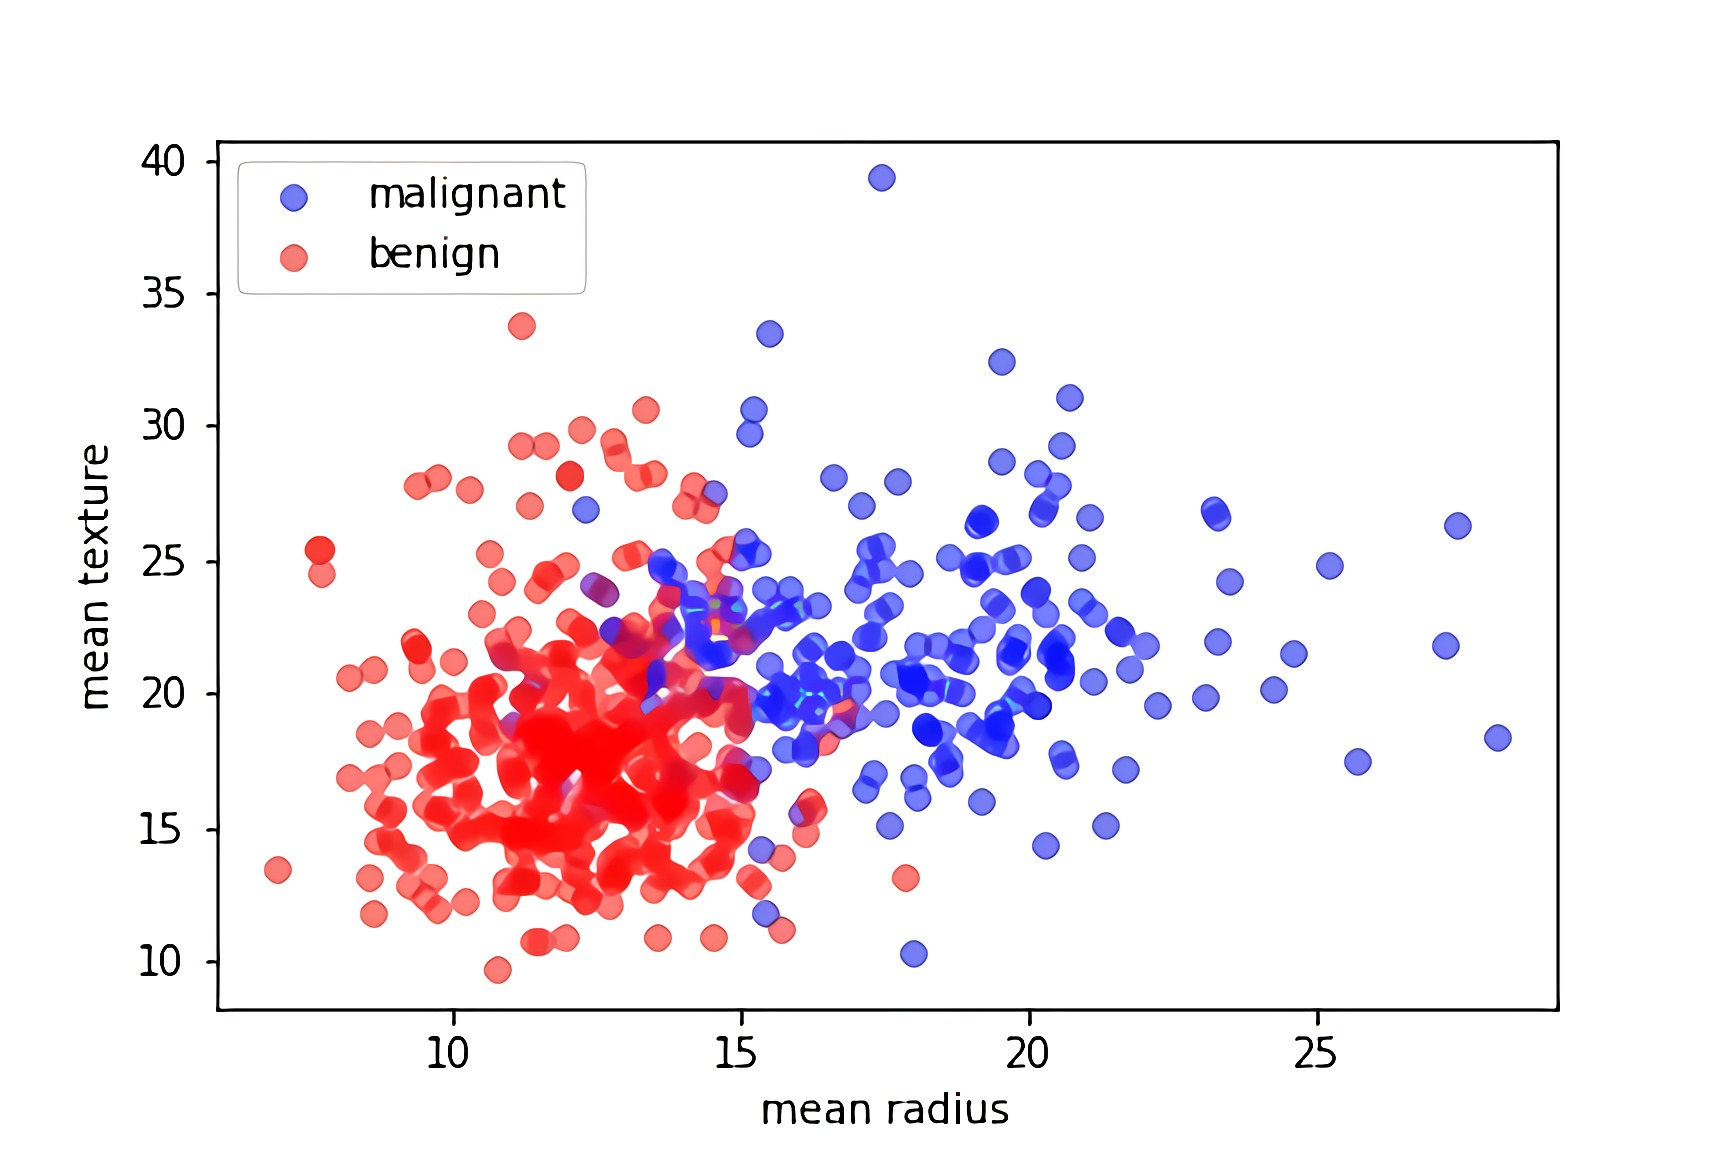
\includegraphics[width=\textwidth]{images/fig1}
        \caption{Class distribution on the dataset with IR=1.684}
        \label{fig1}
    \end{minipage}
    \quad
    \begin{minipage}{0.45\textwidth}
        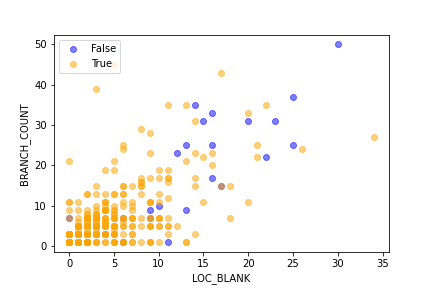
\includegraphics[width=\textwidth]{images/fig2}
        \caption{Class distribution on the dataset with IR=12}
        \label{fig2}
    \end{minipage}
\end{figure}

The class imbalance problem means one class contains a small number of data instances, but the other one is represented by a large number of data instances \cite{10}. In practical situations, the ratio between these two classes may be substantial, similar to 1:100, 1:1000, 1:10000, or even higher \cite{1}. Figure \ref{fig1} and Figure \ref{fig2} show the difference between two datasets with an  Imbalance Ratio(IR) of 12 and 1.684,  respectively. In addition, it should be noted that, under some specific circumstances, the problem of class imbalance has an internal cause \cite{1}. For example, Haibo He and Edwardo A. Garcia gave an example of cancer classification in their 2009 work \cite{17}. Such an example demonstrates that, in the screened population, the prevalence of cancer is particularly low, which leads to the class imbalance problem in the collected data, in which one disease state is underrepresented \cite{17}. However, due to the limitation of the data collection process, in areas where there is no inherent imbalance, there is also the possibility for the occurrence of a class imbalance problem: namely, the way of choosing the data by researchers (for example which data and in what quantity) and the imbalanced cost for different errors can also lead to class imbalance problems \cite{1}. Such a situation may vary from case to case \cite{1}. Affected by these conditions, normal classifiers are often confused by the majority class and ignore the minority class \cite{1}. Additionally, for the percentage of examples available for each class, most real-world data processed using non-linear classification strategies are imbalanced, which may cause the algorithm to learn overly complicated models that overfit the data and have almost no correlation \cite{2}. This issue is critical since it leads to a significant barrier in the performance achieved by basic learning methods which assume that the class distribution is balanced \cite{2}.

Classification in medical diagnostics can aid in disease diagnosis and predict outcomes in response to treatment \cite{3}. For instance, with Computer Aided Decision(CAD) systems, a physician is able to diagnose a patient with the help of computer algorithms and classification is one of the most common tasks performed by the CAD system \cite{4}. However, data collection in the medical sector is associated with a number of challenges and practical limitations. The collection of patient data is time-consuming \cite{4} and the collection of balanced model training data is difficult where there is low prevalence of the disease \cite{7}. In addition, the inherent heterogeneity, incompleteness, and high-dimensional nature of healthcare/medical data can also lead to challenges \cite{5}. The medical data is often heterogeneous where patient records contain various data types, including images, real and integer with different ranges, and text types \cite{5}.

Many classification algorithms have been developed recently and used to detect and predict some common diseases such as diabetes, Parkinson's disease and vertebral column pathologies, which has brought significant trouble and pain to a tremendous number of patients \cite{6}.

Study \cite{5} addressed the problems of imbalanced healthcare data on the diagnosis of a brain tumor. In this study, a new approach to data mining is adopted, combining feature selection and ensemble classification. Study \cite{3} introduced a novel voting class weight algorithm called CWsRF based on random forest algorithm (RF), which focuses on the challenge of identifying the minority class sufficiently in medical applications and can be applied to the detection of diseases, such as breast cancer, or medical images classification. Study \cite{8} offers an innovative ensemble learning paradigm for the early detection of diseases with imbalanced data that functions equally as well as or outperforms the other state-of-the-art comparison algorithms, such as support vector machines and random forest. This algorithm is the first comprehensive ensemble learning technique that involves multiple SVM diversity structures for classification, which can prevent the generation of noisy instances and effectively re-balance the input data \cite{8}. 

\section{Related Work on Imbalanced Classification}
\subsection{Sampling Methods}
Resampling, which involves creating a new transformed version of the training set of an imbalanced dataset, offers a set of practical and straightforward approaches to provide a more balanced data distribution \cite{9}. All these approaches can be classified into three groups: Oversampling techniques, Undersampling techniques, and Hybrids techniques \cite{10}. In the first case, oversampling, the original dataset will be augmented by replicating the selected instances or creating new instances from the existing one, while with undersampling methods, a set of data (usually majority class samples) will be removed from the original set. The hybrid methods are a combination of both from sampling algorithms \cite{10}. Among these three groups, random oversampling and random undersampling are non-heuristic and the simplest approaches; the former case has the drawback of overfitting, and in the case of the latter, the omission of some crucial samples pertaining to the majority class may occur due to the removal of examples \cite{17}. Moreover, informed undersampling based on the traditional undersampling method aims to deal with information loss deficiency. The \textit{EasyEnsemble} and \textit{BalanceCasade} are two applications of this algorithm with good performance \cite{12}. Additionally, synthetic sampling with data generation is also a useful approach to improve data distribution. Some of the renowned algorithms in this area are the \textit{SMOTE} \cite{13} and the \textit{Borderline-SMOTE} \cite{15}, which was applied to various situations with a great deal of success. In addition, to deal with the overlapping introduced from sample methods, data cleaning techniques have been used practically \cite{17}. \textit{Tomek links} \cite{16} is representative of this kind of method. 

\subsection{Cost-Sensitive Learning Methods}
Sampling methods try to improve the balanced level of the dataset, while cost-sensitive learning methods are utilized to deal with different misclassification errors that incur different penalties to find the optimal decision. The foundation of these decisions is the cost matrix, which is fundamental to the cost-sensitive learning methodology \cite{17,18}. Table \ref{tab1} illustrates the structure of a binary classification cost matrix. The positive category (class label 1) denotes the minority and the negative category (class label 0) represents the majority. If $m$ stands for the predicted label and $n$ stands for the actual label, so the $C(m, n)$ is the cost of predicting a class $n$ sample as class $m$. For example, $C(1,0)$ represents the cost of predicting a negative instance as positive. In view of the cost matrix, the purpose of this type of learning method is explained to create a model with minimal overall misclassification costs \cite{19,20}.
\begin{table}[h]
    \centering
    \begin{tabular}{|c|c|c|}
    \hline
                     & Actual negative & Actual positive \\ \hline
    Predict negative & $C(0,0)$        & $C(0,1)$        \\ \hline
    Predict positive & $C(1,0)$        & $C(1,1)$        \\ \hline
    \end{tabular}
    \caption{Cost Matrix for Binary Classification}
    \label{tab1}
\end{table}

Bearing in mind most traditional classifiers assume that the misclassification has the same cost for false negative(FN) and false positive(FP) \cite{18}. However, real-world scenarios are not so ideal. Conceptually, in certain situations, the cost of incorrect labeling for a sample should always be higher than a correct one \cite{18}. For instance, in cancer diagnosis, where a patient who does have a certain kind of cancer is classified as negative(FN), this error could be much more serious and expensive than regarding a non-cancer patient as positive(FP), which can be corrected by further medical examinations; the former situation may lead to a worse patient condition or the even more severe outcome of losing his life \cite{21}. In another scenario, the cost of not mailing to potential buyers is higher than mailing to some non-buyers  \cite{19}. From this, it can also be illustrated that costs are not necessarily only monetary but also can be the severity of an illness or the wasting of time \cite{18}. 

The cost matrix values should be defined with care because the supplied cost matrix can strongly impact effectiveness \cite{10}. However, in many cases, the cost of classification errors cannot be described clearly. The determination of a given domain's cost representation can be a challenge and, under some circumstances, impossible \cite{17}. There may be a problematic accession to a domain expert or a lack of available prior information on the cost matrix during the classifiers' training process, which is a common phenomenon when cost-sensitive learning is utilized to deal with the class imbalance problem \cite{10}. 

Cost-sensitive learning techniques can be categorized into two families: \textit{Meta-learning} (including two aspects: thresholding and sampling) and \textit{Direct methods} \cite{20}. The principle of the former category is to create a ``wrapper'' to turn existing cost-insensitive classifiers into cost-sensitive classifiers, and in the latter case, classifiers that are cost-sensitive in themselves are constructed \cite{20}. 

The \textit{cost-sensitive decision trees} which have taken account of misclassification during pruning are popularly used as direct methods for detecting card fraud when the cost to misclassify could vary \cite{20,22}. \textit{MetaCost} \cite{23} can be viewed as a representative thresholding tool in the case of thresholding. \textit{Weighting} \cite{24} is one implementation of the sampling methods, in which examples of the minority are assigned high weights according to their proportion.

\subsection{Ensemble Learning Methods}
In 2004, a statistician named James Michael Surowiecki presented in his study \cite{34} that, under certain controlled circumstances, the decisions or predictions made by groups of humans often outperform those made by a single individual. 

The ensemble methodology is used in classification to enhance the output of an individual classifier, which is likely to ask multiple ``experts'' for help: the key idea is to train multiple classifiers and then combine them to achieve an overall classification that overtakes each indivudual classification to produce the final decision \cite{26}. Therefore, the predictions of all members of this ensemble, known as classifier fusion or aggregation are considered in the combining step, in order to classify a new unknown example \cite{10}. In 1979, Dasarathy and Sheela proposed one of the earliest work on ensemble learning \cite{30}. In \cite{30}, the partition of the feature space with two or more classifiers was discussed. Later in 1990, Hansen and Salmon introduced the idea that \textit{ensemble artificial neural networks (ANNs)} with similar configurations can improve a single classifier's generalization performance \cite{31}. Furthermore, the ensemble learning approach was successfully applied to various industries, including medical diagnosis \cite{27}, cheminformatics \cite{28}, bioinformatics \cite{29} and so forth. \textit{Bagging and Boosting} are the two most practical techniques of ensemble learning, which apply instance partitioning methods \cite{36}.

\textit{Bagging} is the abbreviation of Bootstrap Aggregating introduced by Breiman in 1996 \cite{37}, which is a simple but successful method for building a set of classifiers that are suitable not only for dealing with binary, but also multi-class classification \cite{26,33}. In detail, every single classifier in the ensemble is trained on a set of examples which are taken with replacement from the training set \cite{26,33,37}. The base classifier can be trained by using the base learning approach with each set \cite{33}. Major voting is used to generate the ultimate prediction for the composite bagging classifier \cite{26}. Study \cite{33} indicates that, due to the generation of data samples with the bootstrap sampling \cite{37}, there is a large overlap among all data samples. A stable learner (a base algorithm that is intensive to perturbation on training sets) may lead to a set of classifiers whose predictions are very similar with no improvement in generalization after the combination \cite{26,33}. Therefore, a relatively unstable learner should be utilized to ensure the diversity among the ensemble classifiers under this scenario so that sufficiently different decision boundaries can be obtained for small perturbations in different training sets. Random Forests \cite{39} is an extension of the bagging algorithm generated from individual decision trees, whose specific training parameters that can be bootstrapped replicas of the training data, as in bagging, vary randomly \cite{38}.

The word \textit{boosting} refers to a group of algorithms which can transform weak learners (an algorithm generating classifiers that outperform random guessing) to strong learners(low error with high confidence for all class concepts), proven by Schapire in his 1990 study \cite{40}. Similar to Bagging, boosting also generates an ensemble classifier by applying resampling methods on data and is later combined with major voting \cite{26,38}. Freund and Schapire introduced one of the representative works of boosting in 1997, named \textit{AdaBoost}(Adaptive Boosting) \cite{41}, which applies an iterative process to simple boosting in order to improve performance. This approach focuses on the instances which are much more complex to classify. To be clear, in \textit{AdaBoost}, a new dataset, in which more weight is assigned to the instances that are misclassified by the previous classifier and less weight is assigned to the one with a correct prediction, is used for training each subsequent classifier \cite{42}.

\subsection{An Overview of Algorithms on Imbalanced Classification}
\subsubsection{Classical Imbalance Classification Algorithms}
\textbf{\textit{Synthetic Minority Oversampling Technique(SMOTE)}} \cite{13} addresses the class imbalance problem by generating synthetic samples in feature space (Fig \ref{fig3} SMOTE working procedure illustrates the detail of this procedure). One minority class example $s_{1}$ will be selected randomly and then its $k$ nearest neighbors in minority class will be screened out; a line segment is formed between one of these $k$ neighbors $s_{2}$, which is selected at random, and $s_{1}$ in the feature space \cite{13}. SMOTE creates the synthetic samples through a convex combination of $s_{1}$ and $s_{2}$ \cite{51}. As described in \cite{61}, random undersampling is suggested to be used to curtail the size of the majority in the first instance. Next, \textit{SMOTE} is utilized on the training set to align the class distribution. This approach combined with random undersampling is proven to outperform the plain undersampling \cite{13}. 
\begin{figure}[h]
    \centering
    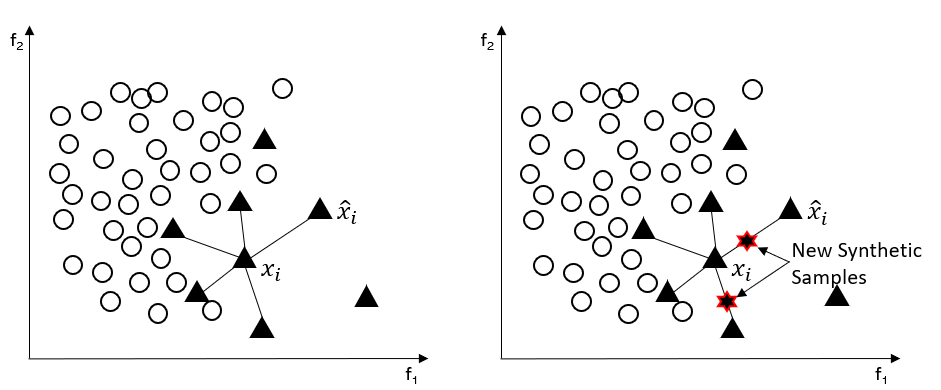
\includegraphics[width=\textwidth]{images/fig3}
    \caption{SMOTE working procedure \cite{100}}
    \label{fig3}
\end{figure}

\textbf{\textit{AdaBoost}} \cite{63} is a boosting ensemble learning approach utilized to deal with the class imbalance problem; the key principle behind it is to enhance the weak learner gradually into a strong learner. This is implemented by varying the sample weight, which indicates its importance in the classifier training process, stage by stage. Fig \ref{fig4} shows the process of combining the ultimate classifier.
\begin{figure}[h]
    \centering
    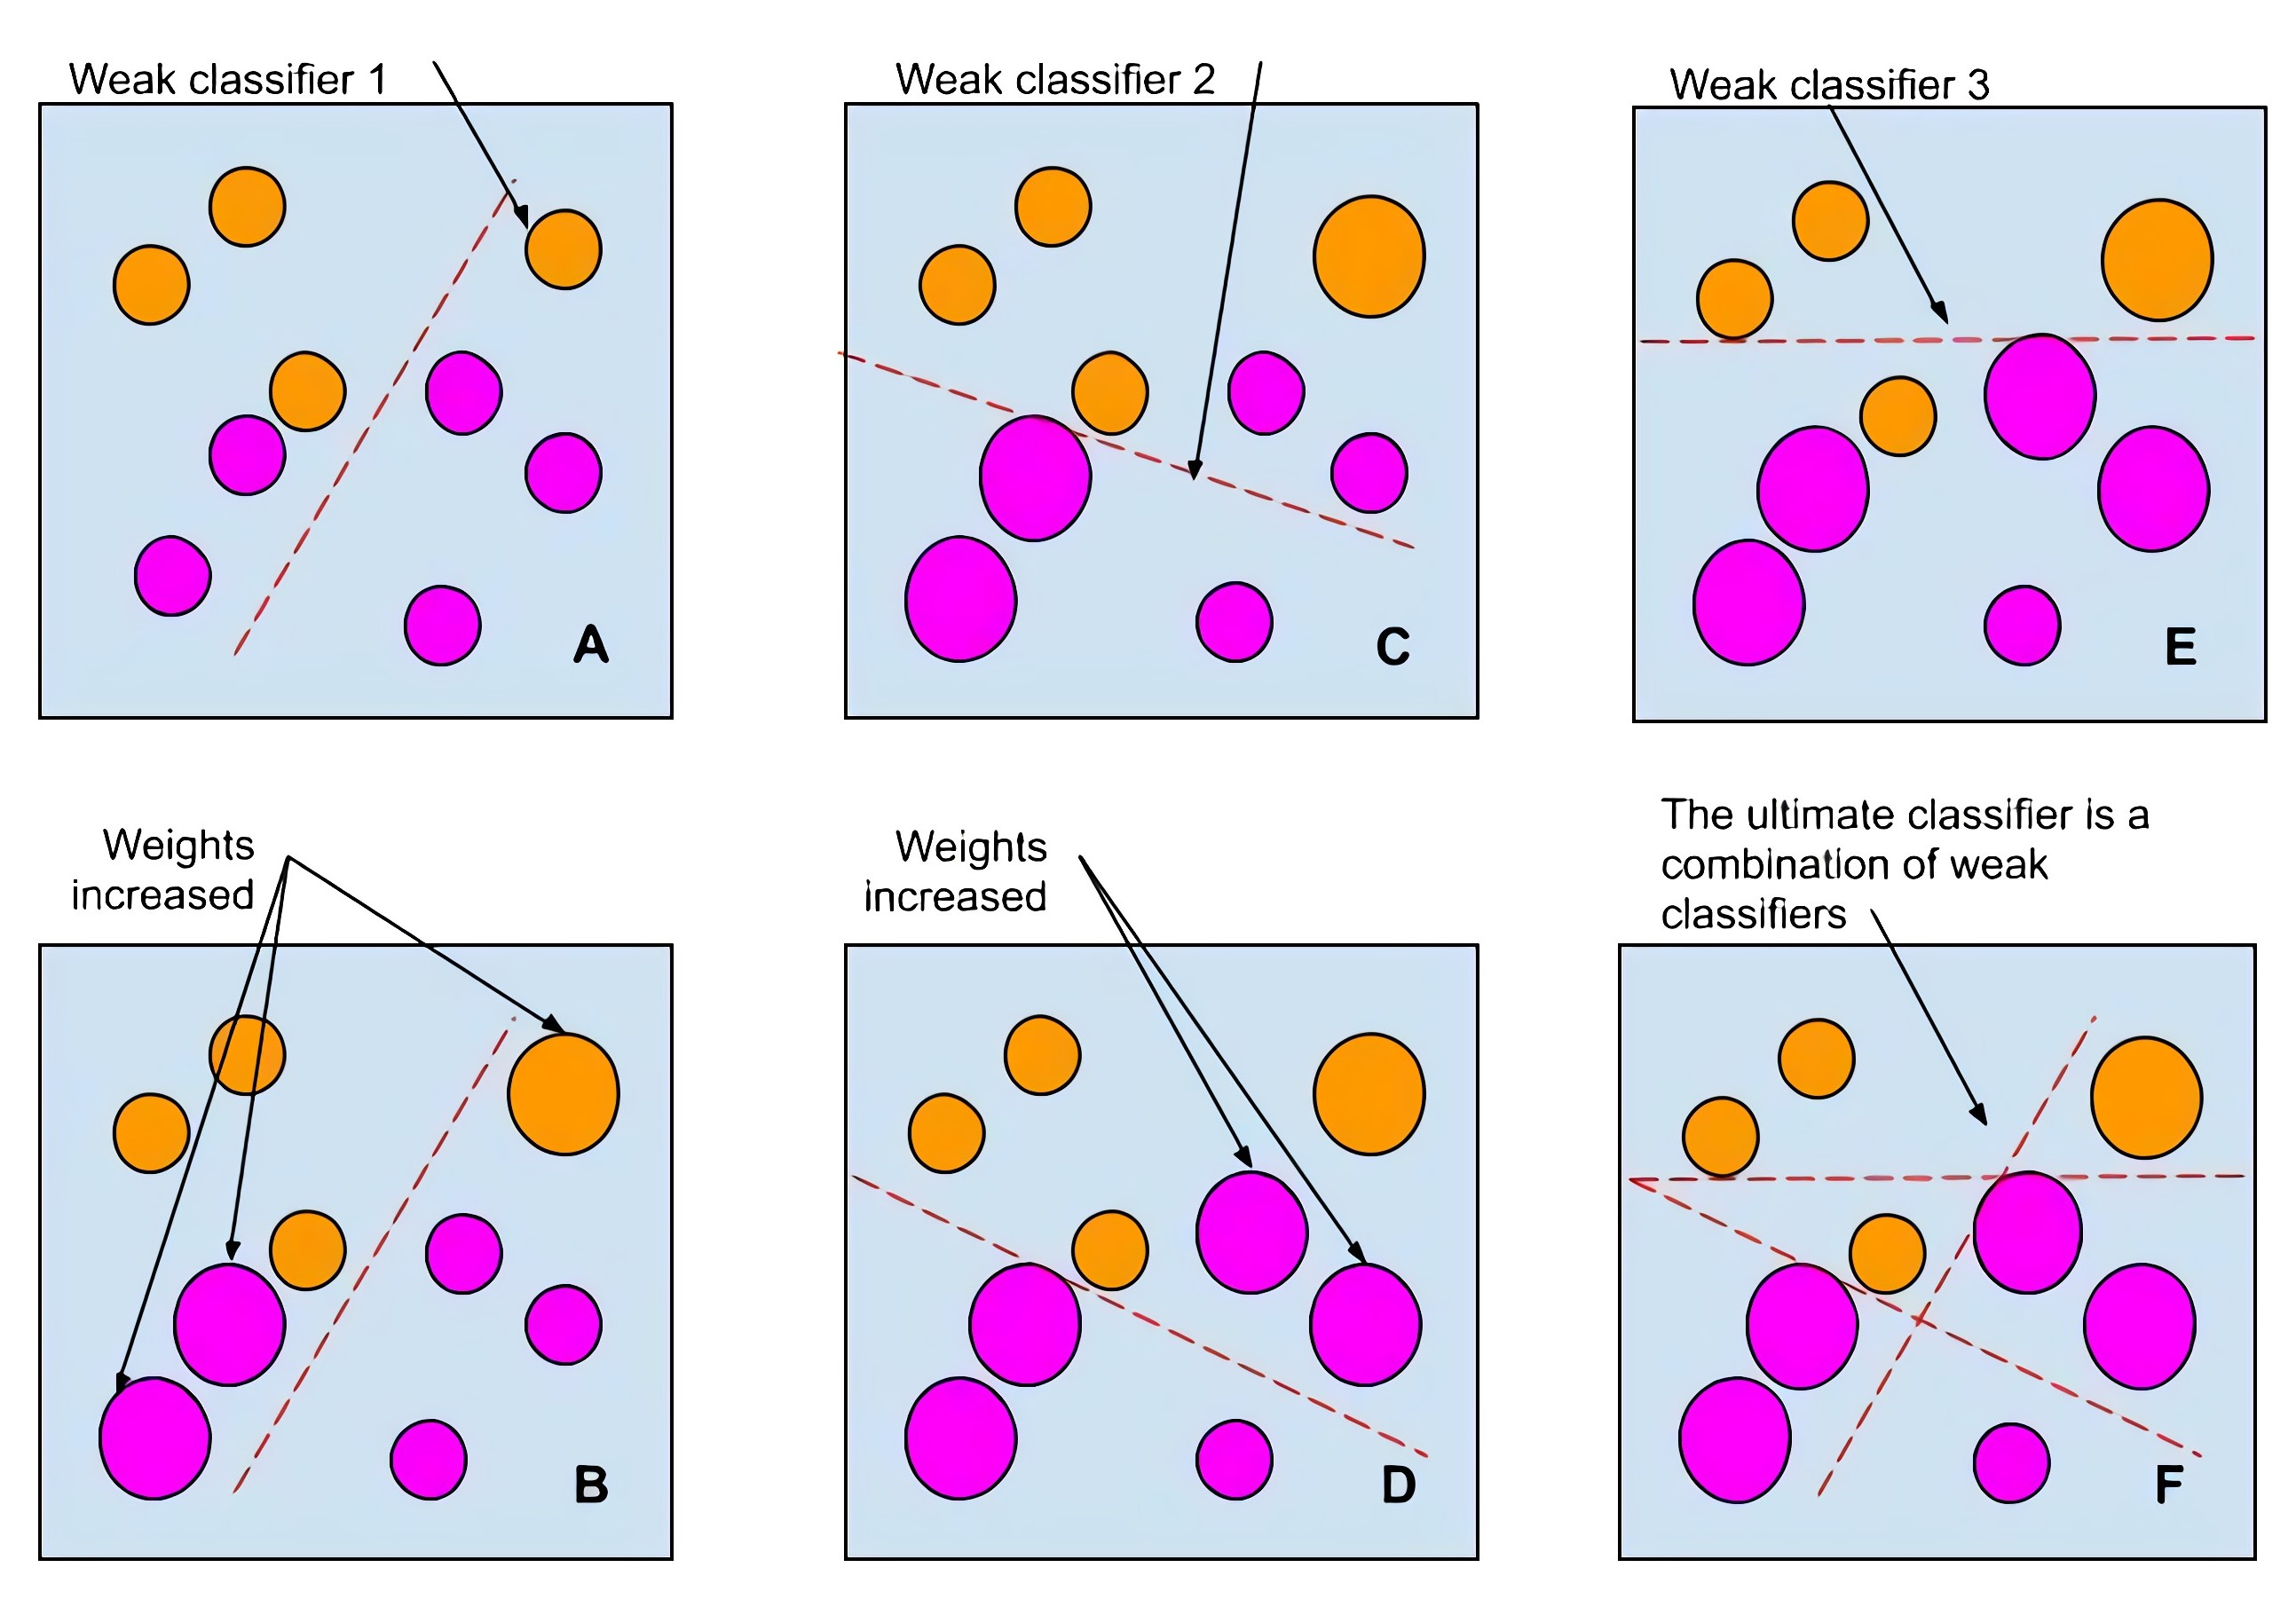
\includegraphics[width=\textwidth]{images/fig4}
    \caption{The process of the combination of the ultimate strong learner in \textit{AdaBoost}}
    \label{fig4}
\end{figure}

\textbf{\textit{Majority Weighted Minority Oversampling Technique (MWMOTE)}} \cite{62} balances the class distribution also by generating synthetic examples. Unlike SMOTE, this approach creates synthetic examples from a weighted minority class through a clustering approach; and the weight of each important minority sample is chosen on the basis of its Euclidean distance to the nearest majority class sample \cite{62}.

\textbf{\textit{RUSBoost}} \cite{64}, a combination of data sampling and boosting algorithm, is based on \textit{SMOTEBoost} \cite{68} that balances class distribution through \textit{SMOTE} and works on improving classifier performance with the balanced data under the help of \textit{AdaBoost}.  Instead of \textit{SMOTE}, this hybrid approach utilizes random sampling(RUS) to achieve increased performance \cite{64}.

\textbf{\textit{CAdaMEC}} \cite{67} is proposed upon \textit{AdaMEC} \cite{66}(a cost-sensitive algorithm) through an appropriate calibration with Platt scaling.

\textbf{\textit{MetaCost}} \cite{23} is one of cost-sensitive learning models through wrapping a cost-minimizing method, which has no restriction on the number of classes or arbitrary cost matrices. This procedure relabels the instances in the training set with the class labels that have estimated minimal-cost, then the new replacement training set will be applied to the error-based learners \cite{23}.

The principle of \textbf{\textit{cost-sensitive decision tree(csDCT)}} is to consider minimizing two separate costs: the test cost of the \textit{i}th feature and the cost of misclassification of the sample \cite{10}.

\subsubsection{Recent State-of-the-art Imbalance Classification Algorithms}
\textbf{\textit{Self-paced Ensemble Classifier}} \cite{96} is an effective ensemble classifier generated by self-paced harmonizing data hardness through undersampling. It has been proven that this model can achieve robust performance even when the classes are highly overlapped and the data distribution highly skewed \cite{96}.

\textbf{\textit{DDAE}} \cite{73} is a novel model to address the class imbalance problem consisting of several classical approaches, including resampling, data metrics learning, cost-sensitive-learning, and ensemble learning. More detail will be described in section 3.2.1.

\textbf{\textit{Iterative Metric Learning (IML)}} \cite{72} focuses on the exploration of a stable neighborhood space for each of the data samples in the testing set. To achieve this, the proposed procedure utilizes an iterative metric learning technique \cite{72}. More detail will be described in section 3.2.2.

\section{Evaluation Metrics for Imbalanced Classification}
Evaluation of classification performance always plays a significant role in guiding and learning performance \cite{44}. \textbf{\textit{Confusion matrix}} \cite{104} provides a deeper understanding of predictive model performance through the results of the predictions so that the types of error can be more clearly observed. Table \ref{tab2} shows the structure of a confusion matrix for binary classification. Table \ref{tab3} shows the measures derived using the confusion matrix from Table \ref{tab2}
\begin{table}[h]
    \centering
    \begin{tabular}{|c|c|c|}
    \hline
                     & Actual negative                              & Actual positive                              \\ \hline
    Predict negative & \textit{TN}(True Negative)  & \textit{FN}(False Positive) \\ \hline
    Predict positive & \textit{FP}(False Positive) & \textit{TP}(True Negative)  \\ \hline
    \end{tabular}
    \caption{Confusion Matrix for Binary Classification}
    \label{tab2}
\end{table}

Cesar Ferri et al. categorized evaluation metrics into three groups in their 2008 work \cite{45}: \textit{probability metrics}, \textit{ranking metrics} and \textit{threshold metrics}. In this paper, two groups of metrics, threshold and ranking metrics, are applied to evaluate the model performance.

Thresholding metrics, which quantify the classification prediction error, focuses on the generalization ability of the trained classifier through the quality of the trained classifier when used to predict unknown examples \cite{46}. The most common threshold metric is the \textbf{\textit{accuracy}} of classification applied in most conventional applications; nevertheless, accuracy is inappropriate for evaluating the imbalanced dataset since it is simple for a classifier that only predicts the majority to yield a low error \cite{47}. 

Sensitivity-specificity metrics are practical thresholding metrics for imbalanced classification that are applied by several researchers \cite{49,50}. As defined in Table \ref{tab3}, \textbf{\textit{specificity}} means the true negative rate. \textbf{\textit{Sensitivity}}, the complement to specificity, describes the true positive rate. The \textbf{\textit{geometric mean (G-mean)}} calculated through the combination of sensitivity and specificity, which has been used by Kubat and Matwin in their 1997 paper \cite{58}, can balance both concerns. Sensitivity, Specificity and G-mean are taken into account when both positive and negative classes are meaningful at the same time \cite{48}. In addition, Precision-Recall metrics arising from the fields of information retrieval are utilized when the output of the minority(class positive) is more crucial \cite{52}. In this paper, \textbf{\textit{F1}} (the value of $\beta$ in $F_{\beta}$-\textit{Measure} is 1) is utilized as one of the most important evaluation metrics.
\begin{table}[h]
    \centering
    \renewcommand\arraystretch{2.5}
    \begin{tabular}{|m{0.3\textwidth}<{\centering}|m{0.6\textwidth}<{\centering}|}
    \hline
    Metrics                       & Formula                                                                                                                                 \\ \hline
   \textit{Accuracy}             & $\dfrac{T P+T N}{T P+T N+F P+F N}$                                                                                             \\ \hline
    \textit{Error Rate}           & $\dfrac{F P+F N}{T P+T N+F P+F N}$                                                                                             \\ \hline
    \textit{Precision}            & $\dfrac{T P}{T P+F P}$                                                                                                         \\ \hline
    \textit{Recall (Sensitivity)} & $\dfrac{T P}{T P+F N}$                                                                                                         \\ \hline
    \textit{$F_{\beta}$-Measure}  & $\dfrac{\left(1+\beta^{2}\right) * \text { Precision } * \text { Recall }}{\beta^{2} * \text { Precision }+\text { Recall }}$ \\ \hline
    \textit{Specificity}          & $\dfrac{T N}{T N+F P}$                                                                                                         \\ \hline
    \textit{Geometric Mean}       & $\sqrt{\text { Sensitivity } * \text { Specificity }}$                                                                         \\ \hline
    \end{tabular}
    \caption{Evaluation Metrics based on Confusion Matrix}
    \label{tab3}
\end{table}

Nonetheless, threshold metrics are not suitable when the distribution of categories observed in the training dataset does not match the distribution of the test set and the actual data, which can make the performance misleading \cite{51}. 
\begin{figure}[h]
    \centering
    \begin{minipage}{0.49\textwidth}
        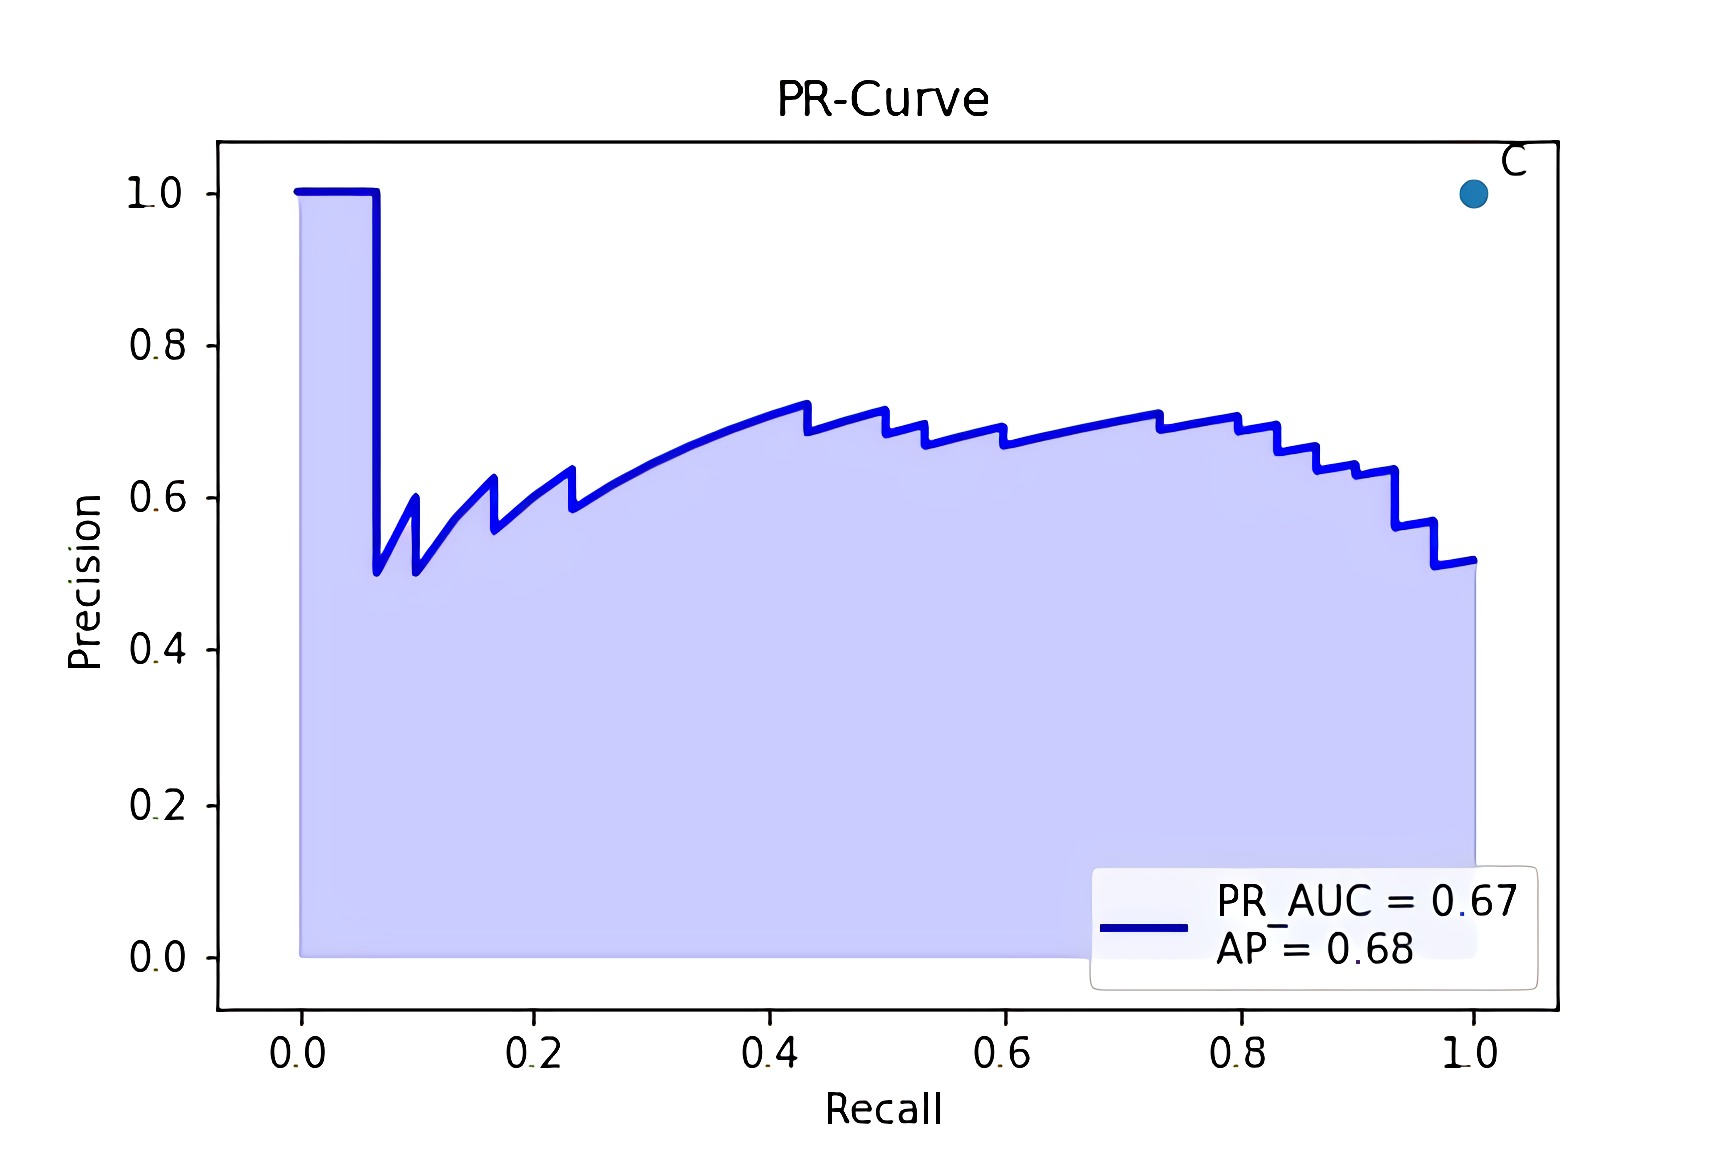
\includegraphics[width=\textwidth]{images/fig5}
        \caption{An example of PR Curve}
        \label{fig5}
    \end{minipage}
    \begin{minipage}{0.49\textwidth}
        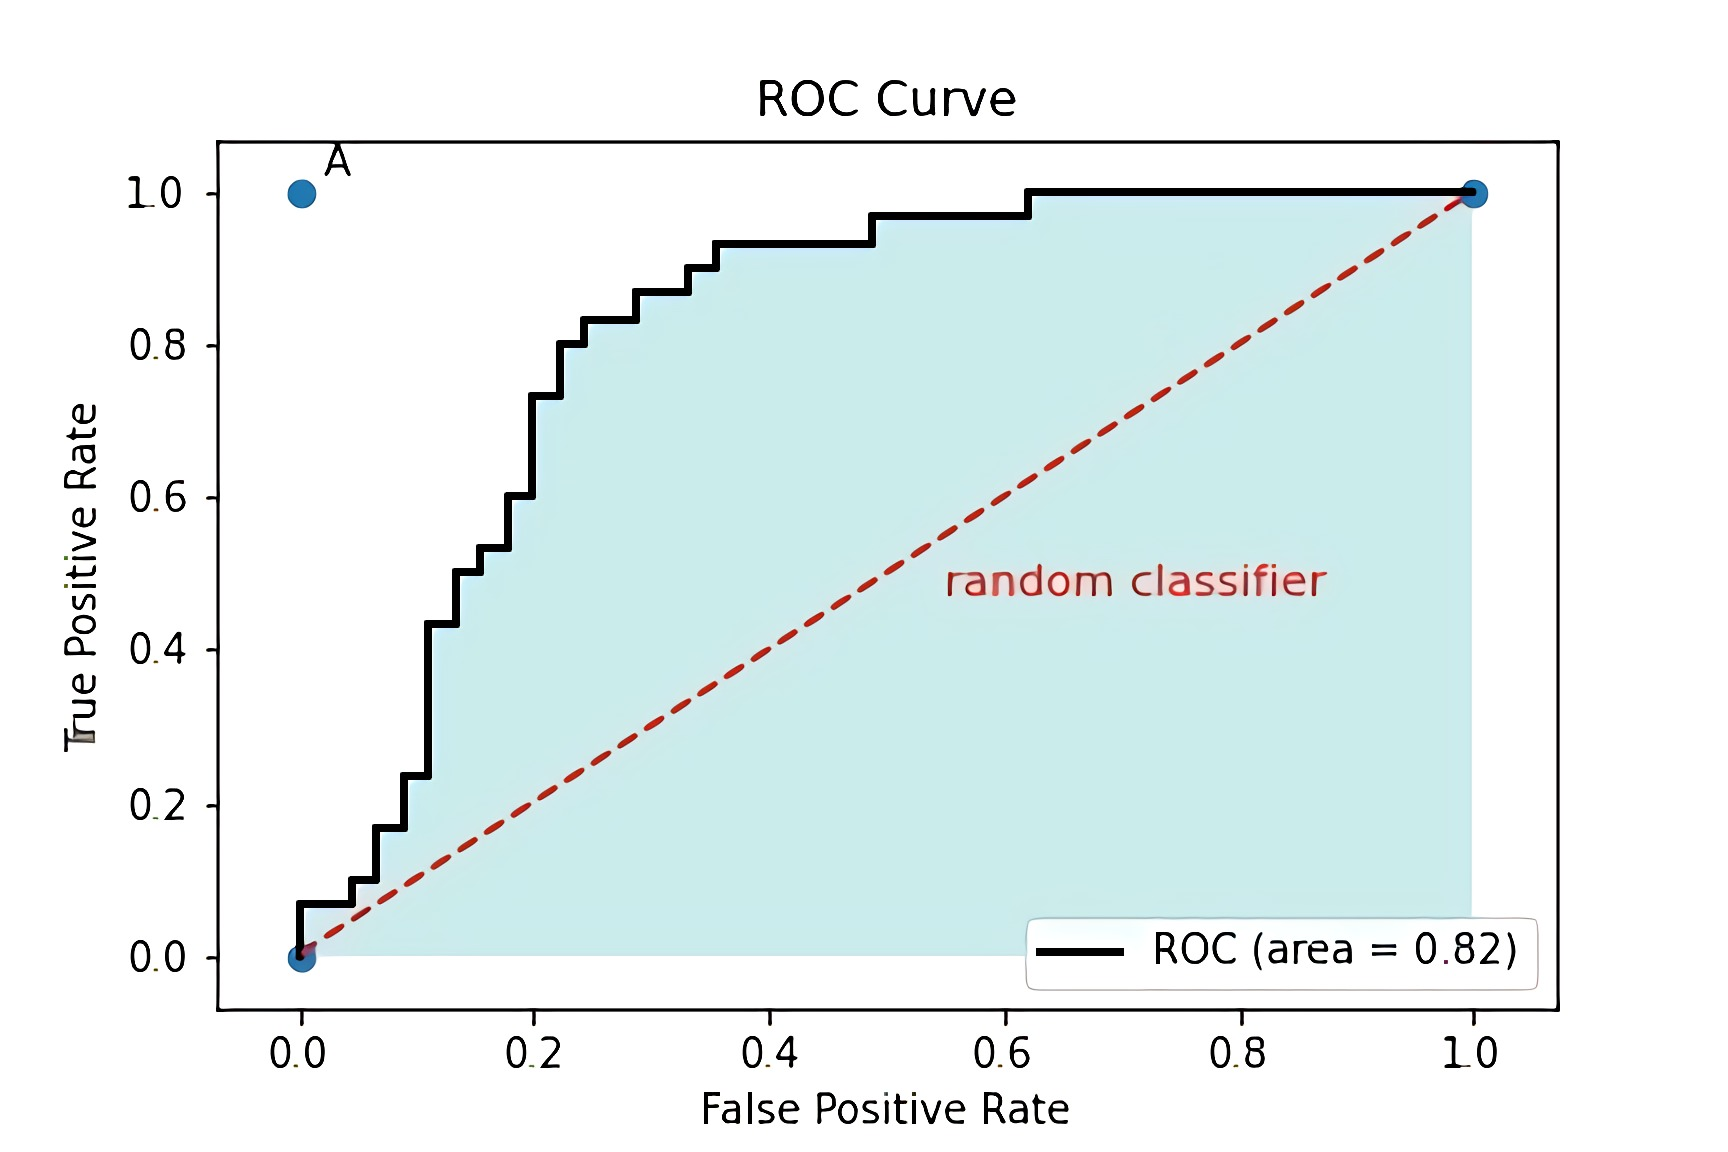
\includegraphics[width=\textwidth]{images/fig6}
        \caption{An example of ROC Curve}
        \label{fig6}
    \end{minipage}
\end{figure}

The ranking metrics focuses on how effectively the base classifiers rank the examples \cite{45}. A numeric score of an example that refers to the probability of being classified as positive is provided by the base classifier, which shows the level of granularity instead of a simple prediction. Different thresholds whose choice affects the trade-offs of both classes' errors can be utilized to test classifiers' performance \cite{10}. \textbf{\textit{Receiver Operating Characteristics (ROC) Curve}} \cite{53} is the most commonly applied ranking metric that is not based on a specific threshold. ROC Curve takes the true positive rate (TPR) and false positive rate (FPR) into account and each point of ROC Curve corresponds to the single classifier performance with a given distribution \cite{17}. The \textbf{\textit{area under the ROC curve (AUCROC)}} is generally applied to measure different classifiers' performance, which is summarized into a single metric \cite{48}. An example of ROC Curve can be observed from Fig \ref{fig6}. Point A $(0,1)$ represents the best performance of the classifier. Therefore, the closer the ROC curve is to A and the more it deviates from the 45-degree diagonal(representing a random classifier), the more successful it is; this also indicates the greater the AUCROC is, the better \cite{53,48}. However, in \cite{17}, it is argued that even a classifier with a high AUCROC can perform poorly in a particular region in ROC space compared with a low AUCROC classifier.

If a dataset is highly skewed, the performance of the algorithm might as observed overly optimistic through a ROC curve \cite{111}. The \textbf{\textit{Precision-Recall (PR) Curve}}, which assesses a more informative representation of performance, is utilized to solve such a limitation \cite{17,54}. PR-Curve is a plot of Recall on the x-axis and Precision on the y-axis \cite{54}, and it can capture the performance of the classifier correctly and effectively if the number of false positives drastically change as the Precision metrics takes the ratio of TP to TP+FP into account \cite{17}. Due to its high level of performances with highly skewed data, it has been applied to the evaluation of performance by many researchers, such as \cite{55,56,57}. Unlike ROC-Curve, whose objective is to be closer to the point $(0,1)$, the highest performing classifier is represented by a PR-Curve residing in the top right of the PR space(point $C(1,1)$) \cite{10}. Similar to AUCROC, the \textbf{\textit{area under the PR Curve (AUCPRC)}} is also a summary of PR-Curve with a single scale value \cite{10}. An example of PR-Curve can be observed in Fig \ref{fig5}.

Recall, Precision, G-Mean, F1 and AUCPRC are applied to evaluate the algorithms' performance in the following experiment.
    %\myemptypage

    \chapter{Methodology}
In this chapter, the structure and implementation processes of the DDAE model (see section 3.1.1) and the Iterative Metric Learning model (see section 3.1.2) are presented in detail.

\section{Algorithm Implementation}
\subsection{DDAE}
In this section, the process of implementing the novel model DDAE\cite{73} is presented in detail from its four components. \textbf{Data Block Construction} is constructed to balance the class distribution. \textbf{Data Space Improvement} improves data space for the training set through \textbf{Largest Margin Nearest Neighbor(LMNN)}\cite{69}. \textbf{Adaptive Weight Adjustment} is inspired by cost-sensitive learning and it generates a weight to make the classifier work better. The last component, \textbf{Ensemble Learning}, utilizes major voting and the weight from Adaptive Weight Adjustment component to determine the ultimate prediction. In this algorithm, \textbf{\textit{k-nearest neighbors rule}}\textbf{(kNN)}\cite{75} will be used as the base classifier.

\subsubsection{Data Block Construction (DBC) Component}
The first step of DBC component is dividing the majority in the training set into several data blocks with a similar size compared to those in the minority in the training set. This can be viewed as an application of undersampling, due to the use of only some of majority samples. Each individually generated data block will be utilized as the training set for each base classifier of the ultimate ensemble classifier. As this approach is introduced to resolve class imbalance problem, the objective of this current component is to achieve better output for each base classifier through balancing the class distribution of each data block. Since one of the significant characteristics of an imbalanced dataset is the huge difference between the class sizes of the majority and minority, DBC applies the concept of oversampling to create more minority samples. This is achieved by copying all the minority samples and placing them in each data block.

Through this procedure, the issue of information loss and overfitting can be improved to some extent,mitigating the arguments against undersampling and oversampling.

The detail of the choice of the number of data blocks $\delta^{*}(\lceil\delta]$ or $\lfloor\delta\rfloor)$ is explained in Chapter 4.
\begin{algorithm}[h]
    \caption{Data Blocks Construction}
    \label{algo1}
    \hspace*{0.02in} {\bf Input:} Training Set $D_{t}$\\
    \hspace*{0.02in} {\bf Output:} A set $B$ of $\delta^{*}$ data blocks
    \begin{algorithmic}[1]
        \State Split the majority and minority instances in the training set into $S_{\text{maj}}$ and $S_{\min}$ respectively\newline Obtain the size of $S_{\text{maj}}$ and $S_{\min}$, denoted as $N_{\text{maj}}$ and $N_{\min}$\newline Obtain the balanced ratio $\delta=N_{\text{maj}} / N_{\min}$
        \State Initialize a set of blocks $B=\left\{B_{1}, B_{2}, \ldots, B_{\delta^{*}}\right\}$\newline $\left(\delta^{*}\right.$ can be considered as $\lceil\delta\rceil$ or $\lfloor\delta\rfloor)$
        \State Divide the majority samples into $\delta^{*}$ parts $\left\{M a_{1}, M a_{2}, \ldots, M a_{\delta^{*}}\right\}$
        \State Copy $S_{\min }$ and $M a_{i}$ into one of the empty data blocks $B_{i}$ which has been created in Step 2.
    \end{algorithmic}
\end{algorithm}

\subsubsection{Data Space Improvement (DSI) Component}
\begin{figure}[h]
    \centering 
    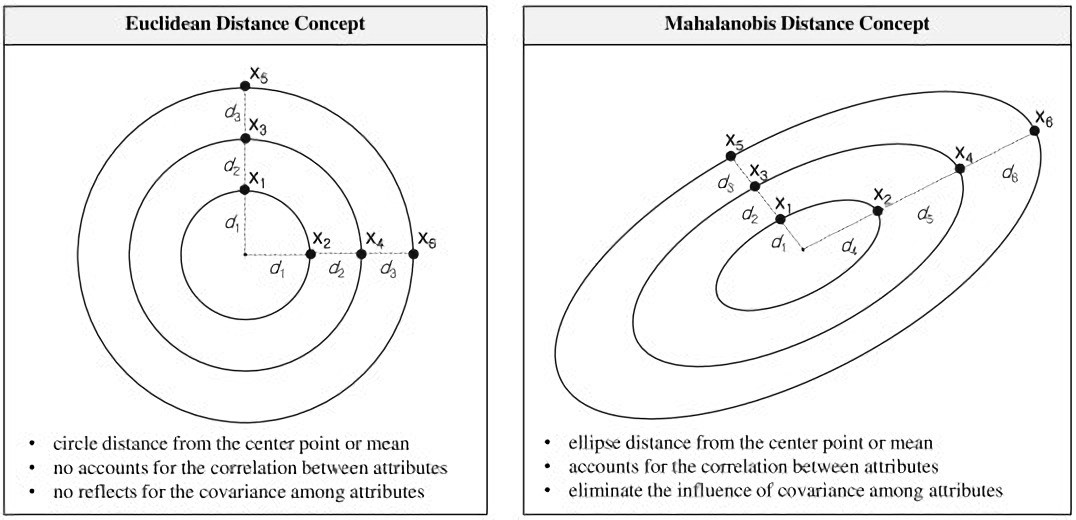
\includegraphics[width=\textwidth]{images/fig7}
    \caption{Comparison of Euclidean Distance and Mahalanobis Distance \cite[Fig.1]{76}}
    \label{fig7}
\end{figure}

In this component, a distance metrics learning algorithm called \textit{large margin nearest neighbor(LMNN)} \cite{69} is utilized to improve the data space for training samples in each data block generated in DBC component.

LMNN, first introduced by Kilian Q. Weinberger and Lawrence K. Saul in their 2009 work \cite{69}, absorbs the particular advantages of several individual models, such as Mahalanobis Metric for Clustering (MMC) [74], Pseudometric Online Learning Algorithm (POLA) \cite{65}, Neighborhood Component Analysis (NCA) \cite{71}. As the classification approach kNN is sensitive with the metric applied to calculate the distances between different examples, LMNN \cite{69} is proposed to learn \textbf{\textit{Mahalanobis distance metrics}} \cite{70} for kNN instead of Euclidean distances used by classical kNN. Figure \ref{fig7} illustrates the difference between these two kinds of distance metric algorithms. The Mahalanobis distance between two data instance points $x$ and $y$, is defined as
\begin{equation}\label{eq1}\footnotemark[1]
    D_{M}(x, y)=\sqrt{(x-y)^{T} \Sigma^{-1}(x-y)}
\end{equation}
\footnotetext[1]{Mahalanobis, P. C. (1936). On the generalized distance in statistics. National Institute of Science of India.}

This proposed approach contains three main parts: a convex loss function, an intention of maximizing margin and the constraints on the distance metric imposed by an accurate kNN algorithm. This, improves the classification accuracy of kNN significantly and it can even be comparable to the SVM classifier on some datasets.

Two simple objectives of LMNN defined in \cite{69} are:

for each training input sample $x_{i}$ and its label $y_{i}$,
\begin{enumerate}
    \item[1.] the label of its k nearest neighbors should be same with $y_i$
    \item[2.] the neighbors with different label should be separated widely. 
\end{enumerate}
\begin{figure}[h]
    \centering 
    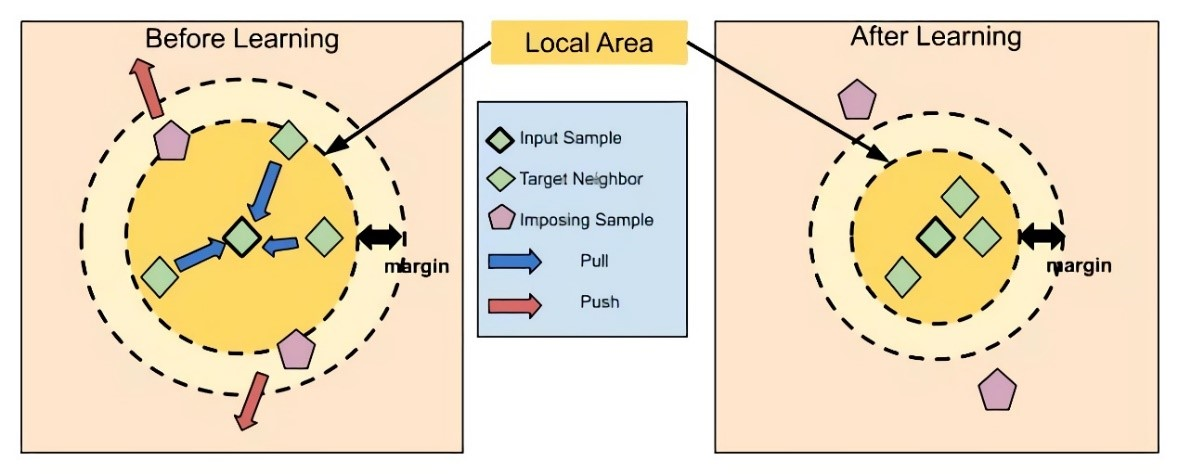
\includegraphics[width=\textwidth]{images/fig8}
    \caption{The procedure of LMNN Distance Metric Learning}
    \label{fig8}
\end{figure}

The first stage is, for each data sample $x_i$, to identify the \textit{target neighbors} that are desired to place close to $x_i$. In other words, there is specific ``margin'' around $x_i$, and other input samples with different labels should be placed further away, so the objective of learning is kind of minimization of the number of these imposing samples which can be introduced through an inequality:
\begin{equation}\label{eq2}\footnotemark[2]
    \left\|L\left(x_{i}-x_{p}\right)\right\|^{2} \leq\left\|L\left(x_{i}-x_{j}\right)\right\|^{2}+1
\end{equation}
\footnotetext[2]{Mahalanobis, P. C. (1936). On the generalized distance in statistics. National Institute of Science of India.}
, with $L$ a linear transformation \cite{69}. For instance, given an input sample $x_i$ with the class label $y_{i}$ and the target neighbor $x_{j}$, the imposing sample $x_{p}$ should satisfy the inequality. The detail of this procedure with $k=3$ as an example can be observed in Figure \ref{fig8}.

Accordingly, the overall loss function should contain two penalizing terms. One of them is used to limit large distances between neighboring input samples with the same class labels, by pulling target neighbors closer to $x_i$, the other is used to penalize small distances between neighboring input samples with different labels by pushing different labeled samples further away. In \cite{69}, the overall loss function for this distance metric learning is a combination of these two mentioned terms, which are denoted as $\varepsilon_{pull}(L)$ and $\varepsilon_{push}(L)$ respectively. With all the previous definitions, it is indicated that these two terms have competing effects, one for attracting the target neighbors and the other for avoiding or repelling the imposing samples. In order to balance these intentions, Weinberger and Saul gives a weighting parameter $\omega$, a positive real number, here. The overall loss function is defined as:
\begin{equation}\label{eq3}\footnotemark[3]
    \varepsilon(L)=(1-\omega) \varepsilon_{p u l l}(L)+\omega \varepsilon_{p u s h}(L)
\end{equation}
\footnotetext[3]{Weinberger, K. Q., \& Saul, L. K. (2009). Distance metric learning for large margin nearest neighbor classification. Journal of Machine Learning Research, 10(2).}
, with a general low-dependence on the value of $\mu$, which can be tuned with the help of cross-validation, for the result of minimizing the loss function.

The first term of loss function is defined as
\begin{equation}\label{eq4}\footnotemark[3]
    \varepsilon_{pull}(L)=\sum\limits_{j \sim i}\left\|L\left(x_{i}-x_{j}\right)\right\|^{2}
\end{equation}
, with $j \sim i$ denoted as each $x_{j},$ which is the target neighbor of $x_{i}$. It should be noted that this term only affects the input samples and their large-distancing target neighbors but not all other input samples with a same class label in the training set.

The second term of the loss function is given as (\ref{eq5})
\begin{equation}\label{eq5}\footnotemark[3]
    \varepsilon_{\text {push }}(L)=\sum\limits_{i, j \sim i} \sum\limits_{p}\left(1-\theta_{i p}\right) \max \left(1+\left\|L\left(x_{i}-x_{j}\right)\right\|^{2}-\left\| L\left(x_{i}-x_{p}\right)\right\|^{2}, 0\right)
\end{equation}
, where a new variable $y_{i p}$ is introduced to show whether the $x_{i}$ and $x_{p}$ belongs to the identified class. In particular, $\theta_{i p}=1$ if and only if $x_{i}$ and $x_{p}$ have the same class label, or $\theta_{i p}=0$. Additionally, the term $\max (m, 0)$ refers to the standard hinge loss. To be specific, if the input sample $x_{p}$ is placed away from $x_{i}$ safely, this means that its hinge loss is with a negative argument so that there will be no effect on the overall loss function. 

The last step of this approach is the minimization of this overall loss function. In \cite{69}, this can be achieved through gradient descent in the element of $L$.

\subsubsection{Adaptive Weight Adjustment (AWA) Component}
Since most ensemble learning approaches assume that the significance of each base classifier (or the weight of each base classifier) is totally equal \cite{32}, the purpose of this AWA component is to find an appropriate overall class weight generated using the data coming from each data block \cite{73}.

In \cite{73}, a definition called \textbf{\textit{unstable confusion matrix}} with a similar structure as classical confusion matrix (see Table \ref{tab2}) is first introduced in this component, which can be observed in Table \ref{tab4}. In detail, the figure for $u(0,0)($resp. $u(0,1))$ is the number of unstable samples with negative as real label and predicted as negative(resp. positive) and so the figure for $u(1,1)($resp. $u(1,0))$ represents the number of \textit{unstable samples} with positive as the real label and classified as positive(resp. negative).
\begin{table}[h]
    \centering
    \begin{tabular}{|c|c|c|}
    \hline
                     & Actual negative              & Actual positive              \\ \hline
    Predict negative & $u(0,0)$ (True Negative)     & $u(1,0)($ False Positive $)$ \\ \hline
    Predict positive & $u(0,1)($ False Positive $)$ & $u(1,1)$ (True Negative)     \\ \hline
    \end{tabular}
    \caption{Unstable Confusion Matrix}
    \label{tab4}
\end{table}

But how is an \textit{unstable sample} defined here? First, it should be noted that, as the kNN classifier is utilized as a base classifier in this DDAE model, it is probable that the k-nearest neighbors for each data sample are not labeled similarly \cite{73}. One particular instance of this is when the number of two class samples among these k neighbors is not very different. For instance, if $k$ is assumed as 7, and among the 7 nearest neighbors of a data sample $s$, there are 3 labeled as negative and the other 4 are labeled as positive. According to the kNN rule, these should be predicted as positive but in reality, this decision can be somewhat ambiguous. So this kind of data sample is called an unstable sample, and in \cite{73}, the absolute difference between the number of these two class samples, so-called \textbf{\textit{positive-negative count difference (PNCD)}}, is introduced to distinguish the unstable sample more formally:
\begin{equation}\label{eq6}\footnotemark[4]
    s \in\left\{\begin{array}{ll}
    \text {unstable samples, } & \text { PNCD }<\rho \\
    \text {stable samples, } & \text { otherwise }
    \end{array}\right., \text{ with }\rho=\left\{\begin{array}{ll}
        1, & k \text { is odd } \\
        2, & \text { otherwise }
        \end{array}\right..
\end{equation}
\footnotetext[4]{Yin, J., Gan, C., Zhao, K., Lin, X., Quan, Z., \& Wang, Z. J. (2020). A Novel Model for Imbalanced Data Classification. In AAAI (pp. 6680-6687).}

To determine PNCD for each test data sample, in each data block, the distances between the specific data sample and each sample in the data block are determined from Euclidean distances.

After finding $k$ nearest neighbors for each test sample, it is easy to calculate the PNCD for it. According to (\ref{eq6}), a judgement will be given as to whether this sample belongs to the set of unstable samples or not. 
\begin{algorithm}[h]
    \caption{Find Neighbors for Test Sample}
    \label{algo2}
    \hspace*{0.02in} {\bf Input:} Test Instance $t,$ Data Block $b_{j}$ with $q$ data samples\\
    \hspace*{0.02in} {\bf Output:} List $neigh$ with $k$ samples(neighbors) 
    \begin{algorithmic}[1]
        \State Initialize an empty lists $distance$
        \For{$j=0$ to $q-1$}
            \State Calculate the distance $dist_{j}$ between $b_{i}[j]$ and $t$
            \State Add ($dist_{j}, j$) into list $distance$
        \EndFor
        \State Sort the list $distance$ according to the first term of each tuple in $distance$
        \For{$z=0$ to $k-1$}
            \State Add $b_{i}\left[\text{distance}\left[z\right]\left[1\right]\right]$ into $neigh$
        \EndFor
        \State \textbf{return} $neigh=\left\{neigh_{0}, neigh_{1}, \ldots, neigh_{k-1}\right\}$
    \end{algorithmic}
\end{algorithm}

As discussed in Chapter 2, the cost of the class positive (minority) is generally higher or more expensive than that of class negative (majority) in imbalanced binary classification. AWA works on the adjustment of weights for the positive and negative predictions and the maximization of the overall gain $g_{overall}$ for the unstable confusion matrix \cite{73}. The weight pair $Weight=\left(Weight_{n}, Weight_{p}\right)$ consists of the weights for negative predictions and positive predictions. $Weight$ is set to $\left(Weight_{\text {default}}, Weight_{\text {default}}\right)$ initially with $Weight_{\text{default}}=1$. If there is an increase with the weights for class positive(resp. negative), $g_{p}\left(\text{resp. } g_{n}\right), g_{\text {overal }}$ is set to $g_{p}\left(\text{resp. } g_{n}\right)$. Otherwise $g_{overall}$ is set to $g_d$.
\begin{equation}\label{eq7}\footnotemark[4]
    \left\{ 
        \begin{array}{l}
            g_{d}=x *(u(1,1)-u(1,0))+(u(0,0)-u(0,1))\\ 
            g_{p}=x *(u(1,1)+u(1,0)+(-u(0,0)-u(0,1))\\ 
            g_{n}=x *(-u(1,1)-u(1,0)+u(0,0)+u(0,1))
        \end{array}    
    \right.
\end{equation}
\footnotetext[4]{Yin, J., Gan, C., Zhao, K., Lin, X., Quan, Z., \& Wang, Z. J. (2020). A Novel Model for Imbalanced Data Classification. In AAAI (pp. 6680-6687).}

In order to maximize the $g_{overall}$, the next step is to find the maximal figure among these three gains. The weight pair $Weight=\left(Weight_{default}, Weight_{default}\right)$ will be updated through a new weight $Weight_{new}=Weight_{threshold}+\gamma$ as follow:
\begin{table}[h]
    \centering
    \begin{tabular}{|c|l|}
    \hline
    $g_d$ maximal: & $Weight=\left(Weight_{default}, Weight_{default}\right)$ \\ \hline
    $g_p$ maximal: & $Weight=\left(Weight_{default}, Weight_{new}\right)$     \\ \hline
    $g_n$ maximal: & $Weight=\left(Weight_{new}, Weight_{default}\right)$     \\ \hline
    \end{tabular}
    \caption{Updating Weight Pair}
    \label{tab5}
\end{table}

with $\gamma$ a small real number larger than 0 and $Weight_{threshold}$ defined as (\ref{eq8})
\begin{equation}\label{eq8}\footnotemark[4]
    Weight_{threshold}=\left\{\begin{array}{ll}
        \hspace{-6pt}\dfrac{\lfloor \frac{\delta^{*}}{2}\rfloor +1}{\lfloor \frac{\delta^{*}}{2}\rfloor -1}, & \text { if } \delta^{*} \text { is odd } \\
    \hspace{-6pt}\dfrac{\frac{\delta^{*}}{2}+1}{\frac{\delta^{*}}{2}-1}, & \text { otherwise }
    \end{array}\right.
\end{equation}
\footnotetext[4]{Yin, J., Gan, C., Zhao, K., Lin, X., Quan, Z., \& Wang, Z. J. (2020). A Novel Model for Imbalanced Data Classification. In AAAI (pp. 6680-6687).}
\begin{algorithm}[h]
    \caption{Determination of overall weight pair}
    \label{algo3}
    \hspace*{0.02in} {\bf Input:} threshold\ $\tau$, $\#default\ weight\ pairs$\footnotemark[5]

    $\hspace{35pt} \#positive\ weight\ pairs$\footnotemark[6], $\#negative\ weight\ pairs$\footnotemark[7]

    $\hspace{35pt}\#all\ weight\ pairs$\footnotemark[8] \\
    \hspace*{0.02in} {\bf Output:} Overall weight pair $Weight^{overall}$
    \begin{algorithmic}[1]
        \If{$\#default\ weight\ pairs\ / \#all\ weight\ pairs\geq \tau$}
            \State \textbf{return} ($Weight_{default},Weight_{default}$)
            \Else
            \If{$\#positive\ weight\ pairs >\#negative\ weight\ pairs$}
                \State \textbf{return} ($Weight_{new},Weight_{default}$)
                \Else
                \State \textbf{return} ($Weight_{default},Weight_{new}$)
            \EndIf
        \EndIf
    \end{algorithmic}
\end{algorithm}
\footnotetext[5]{The number of default weight pairs($Weight_{default},Weight_{default}$)}
\footnotetext[6]{The number of non-default positive weight pairs($Weight_{new},Weight_{default}$)}
\footnotetext[7]{The number of non-default negative weight pairs($Weight_{new},Weight_{default}$)}
\footnotetext[8]{The number of all weight pairs $= 5 + 6 + 7$}

After finishing the above steps, for a single test sample, the result will be $\#data\ block$\footnotemark[9] weight pairs obtained from each data block. The last step(see Algorithm \ref{algo3}) of AWA component is to determine the final overall weight pair $Weight^{overall}=\left(Weight_{n}^{overall},Weight_{p}^{overall}\right)$ for this single test sample, which depends on the frequency of these three different kinds of weight pairs shown in Table \ref{tab5}.
\footnotetext[9]{The number of data blocks}

\subsubsection{Ensemble Learning Component (EL) Component}
The main idea behind this component is ensemble learning (see section 2.2.3), with a weighting parameter determined in AWA component. Multiple base classifiers with major voting technique work on the final decision for each input sample. The number of base classifiers $m$ in this ensemble classifier depends on the number of data blocks generated in DBC component, so is $m=\delta^{*}$.

In particular, this paper focuses on binary classification. At the first stage, for each sample $s$ that needs to be predicted, the number of base classifiers that have predicted it as positive (class label 1) and those as negative (class label 0) need to be counted respectively. This can be denoted as a term $\left(n_{1}, n_{0}\right)$. Namely, for the \textit{i}th base classifier $C L_{i}$, the $r_{(i, label)}(s)=1$ if, and only if, the predicted label for $s$ that made by $C L_{i}$ is same as $label$, with $i$ in range of 0 to $m-1$ and $label\in\{0,1\}$. With this, it is easy to obtain $n_{1}=\sum_{i=0}^{m-1} r_{(i, 1)}(s)$ and $n_{0}=\sum_{i=0}^{m-1} r_{(i, 0)}(s)$.

As introduced in section 2.1.1, the minority or positive class in a class imbalanced dataset always has more impact than the majority or negative class. In order to solve this problem and to enhance the performance of the ensemble classifier, the overall weight $Weight^{overall}=\left(Weight_0^{overall},Weight_1^{overall}\right)$ is utilized to balance these two classes. Thus, the modified major voting technique can be defined as (\ref{eq9}).
\begin{equation}\label{eq9}\footnotemark[10]
    Res(s)=\left\{\begin{array}{ll}
    \hspace{-6pt}label_{0}, & Weight_{0}^{overall} * n_{0} \geq Weight_{1}^{overall} * n_{1} \\
    \hspace{-6pt}label_{1}, & otherwise
    \end{array}\right.
\end{equation}
\footnotetext[10]{Yin, J., Gan, C., Zhao, K., Lin, X., Quan, Z., \& Wang, Z. J. (2020). A Novel Model for Imbalanced Data Classification. In AAAI (pp. 6680-6687).}

\subsection{Iterative Metric Learning(IML)}
In this section, the process of implementing the model IML \cite{72} is presented in detail with its three components. \textbf{Iterative Metric Learning} is constructed to improve the structure of data space through \textbf{Largest Margin Nearest Neighbor(LMNN)} \cite{69}. \textbf{Iterative Training Samples Selection} finds the samples which are more likely to affect the testing data samples. \textbf{Data Matching} determines the most effective neighborhood for each testing data sample. In this algorithm, \textbf{k-nearest neighbors rule(kNN)} \cite{75} will be used as the base classifier. Algorithm \ref{algo4} shows the detail in dealing with imbalanced datasets through IML.

\subsubsection{Iterative Metric Learning}
In this stage, IML also utilizes the LMNN, which was explained in last section, to improve the data space. The objective of this component is same as that of DSI in DDAE, both of which want to separate the data samples with a different class label by a large margin and make the samples with the same class labels close to each other. Unlike DDAE, IML provides an iterative metric learning approach which can locate a more stable neighborhood for the specific testing data.

\subsubsection{Iterative Training Samples Selection}
In this stage, after calculating the distance between each of the samples from training set and the to-be-classified testing sample, the top $d^{p}$ and the top $d^{f}$ training samples for the positive and negative class will be selected; these chosen samples make up the sub training set for the current testing sample \cite{72}.

\subsubsection{Data Matching}
After the first two steps, a temporary neighborhood for the current testing sample has already been discovered. However, to find the most effective training set for the testing sample, the first two steps need to be iteratively repeated. In each iteration, the current discovered neighborhood will be compared with the previously discovered neighborhood. If the ratio between the number of matched training samples and the number of all training samples is greater than the matching ratio, this means that the neighborhood is already stable and the current neighborhood is the appropriate training set for this current testing sample, or the iteration needs to continue until the above condition is met.
\begin{algorithm}[h]
    \caption{IML}
    \label{algo4}
    \hspace*{0.02in} {\bf Input:} Testing set $S^{test}$, Training Set $S^{train}$, matched ratio $\beta$, kNN Classifier $K$\\
    \hspace*{0.02in} {\bf Output:} List of predictions for the given testing set $P$
    \begin{algorithmic}[1]
        \For{$s^{test}$ in $S^{test}$}
            \State Initialize $Pre\_set$ and $Curr\_Set$
            \While{true}
                \State do Metric Learning on $S^{train}$ and update $S^{train}$
                \State do Training Samples Selection and update the $Curr\_Set$
                \State do Data Matching and find the matched samples
                \If{\#matched samples / size$(Curr\_Set) >=\beta$}
                    \State trained the $K$ using $Curr\_Set$, add the prediction into $P$
                    \State \textbf{break}
                    \Else\State $Pre\_set = Curr\_Set$
                \EndIf
            \EndWhile
        \EndFor
        \State \textbf{end for}
        \State \textbf{return} $P$
    \end{algorithmic}
\end{algorithm}
    %\myemptypage

    \chapter{Experiments and Results}
This chapter reports the results of the experiments on imbalanced medical/healthcare datasets in detail. Section 4.1 introduces the datasets used as input. This is followed by section 4.2, which reports the results of all the experiments. Section 4.2.1 presents an overall comparison of all class imbalance classification models. Section 4.2.2 and section 4.2.3 illustrates the result of whether a different imbalanced ratio and the different size of the data set have an impact on the performance of the model. Moreover, in section 4.3, the effectiveness of all components in the DDAE is described. 

\section{Input-Data Used}
\subsection{Source of Datasets}
Eight datasets were collected from the medical or healthcare sector. These are Yeast1vs7, Euthyroid Sick, Thyroid Sick, and Mammographic (MGC), Wisconsin Diagnosis Breast Cancer(WDBC) and Pima Indian Diabetes(PID) from UCI \cite{97}, and two sub datasets of Protein Homology (PH1 and PH2) from KDD Cup 2004 \cite{109}, which are utilized to test the performance of these models. The detail of these datasets is depicted in Table \ref{tab6}. In addition, eight further datasets are employed, including Cm1, Mw1, Pc1, Pc3, Pc4 which are from NASA Metrics Data Program (NASA) dataset \cite{110}, Poker89vs6 and Poker8vs6, which are from KEEL \cite{98}, and Optical Recognition of Handwritten Digits (optdigits) from UCI. All these datasets are imbalanced distributed but with various imbalance ratio(IR), instances and features. The detail of these datasets is depicted in Table \ref{tab25}.

Euthyroid Sick and Thyroid Sick record the patient information of the thyroid disease. In Mammographic (MGC), according to the attributes of BI-RADS and the age of patients, breast and benign breast masses are distinguished. Wisconsin Diagnosis Breast Cancer(WDBC) records the data about diagnostic Wisconsin breast cancer. Pima Indian Diabetes(PID) records the patient information of diabetes disease, and all patients here are females at least 21 years old of Pima Indian heritage. Protein Homology dataset consists of the recording about protein homology. Yeast1vs7 contains the data about  the cellular localization sites of proteins. Poker8v6 and Poker89vs6 are used for poker hands prediction. In addition, optdigits contains normalized bitmaps of handwritten digits from a preprinted form.

\begin{table}[h]
    \centering
    \begin{tabular}{|p{0.2\textwidth}<{\centering}|p{0.15\textwidth}<{\centering}|p{0.2\textwidth}<{\centering}|p{0.1\textwidth}<{\centering}|p{0.15\textwidth}<{\centering}|}
    \hline
    \textbf{Dataset}        & \textbf{\#Class} & \textbf{\#Instances} & \textbf{\#F} & \textbf{IR} \\ \hline
    \textbf{Euthyroid Sick} & 2                & 3,163                & 42           & 9.795       \\ \hline
    \textbf{Thyroid Sick}   & 2                & 3,772                & 52           & 15.329      \\ \hline
    \textbf{PH1}            & 2                & 11,274               & 74           & 7.699       \\ \hline
    \textbf{PH2}            & 2                & 31,296               & 74           & 23.148      \\ \hline
    \textbf{MGC}            & 2                & 11,183               & 6            & 42.012      \\ \hline
    \textbf{Yeast1vs7}      & 2                & 459                  & 7            & 14.3        \\ \hline
    \textbf{WDBC}      & 2                & 768                  & 8            & 1.866        \\ \hline
    \textbf{PID}      & 2                & 568                  & 32            & 1.684        \\ \hline
    \end{tabular}
    \caption{Characteristics of used Datasets from Medical or Healthcare Sector}
    \label{tab6}
\end{table}

\begin{table}[h]
    \centering
    \begin{tabular}{|p{0.2\textwidth}<{\centering}|p{0.15\textwidth}<{\centering}|p{0.2\textwidth}<{\centering}|p{0.1\textwidth}<{\centering}|p{0.15\textwidth}<{\centering}|}
    \hline
    \textbf{Dataset}        & \textbf{\#Class} & \textbf{\#Instances} & \textbf{\#F} & \textbf{IR} \\ \hline
    \textbf{optdigits}           & 2                & 5,620                & 65           & 9.144       \\ \hline
    \textbf{Cm1}            & 2                & 497                  & 21           & 9.354       \\ \hline
    \textbf{Mw1}            & 2                & 403                  & 37           & 12          \\ \hline
    \textbf{Pc1}            & 2                & 1109                 & 21           & 13.4        \\ \hline
    \textbf{Pc3}            & 2                & 1563                 & 37           & 8.769       \\ \hline
    \textbf{Pc4}            & 2                & 1458                 & 37           & 7.191       \\ \hline
    \textbf{Poker89vs6}     & 2                & 1485                 & 10           & 58.4        \\ \hline
    \textbf{Poker8vs6}      & 2                & 1477                 & 10           & 85.882      \\ \hline
    \end{tabular}
    \caption{Characteristics of used Datasets from Other Fields}
    \label{tab25}
\end{table}

\subsection{Data Pre-processing}
As described in section 2.1, the datasets in the real world are generally not as perfect as expected. They can be unreliable or dirty, with lack of attribute values, containing noise (errors or outliers) and inconsistent or duplicate values \cite{82}. The performance of classifiers is dependent on the quality of training data. A dirty or incorrect training set can result in a poor classification model \cite{81}. In order to reduce the impact of these issues on prediction models, data pre-processing, a critical part of data analysis and machine learning, takes a huge amount of time \cite{77}. In this paper, the experiment focuses on the performance of the model, so here only a brief pre-processing is performed on the input datasets.

In \cite{77}, the process of data preparation is depicted in four steps: data integration, data cleaning, data normalization and data transformation. However in other literature, such as \cite{79}, this process is presented more detail and data normalization is seen as a part of data transformation. 

When the data is obtained from multiple data sources, step one is critical wherein all the data collected needs to be integrated \cite{77}. This procedure involves the identification of redundant attributes, in which the size of dataset can be decreased, also reducing the modeling time of further algorithms \cite{77}, as well as the detection of duplication and inconsistency. As some identical instances are seen as different due to errors in the entry step, duplication is a cause of inconsistency which means detection is indispensable \cite{80}.

Data cleaning is performed to deal with dirty data \cite{77}, which includes missing values, incorrect data and data with non-standard representation. A high proportion of this kind of data lead to an ineffective and unreliable algorithm \cite{81}. This procedure can be divided into three parts: missing value processing, outliers processing and noise processing \cite{79}.
\begin{figure}[h]
    \centering 
    \begin{minipage}{0.45\textwidth}
        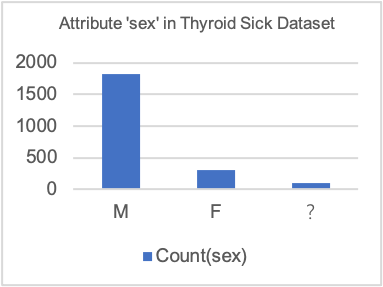
\includegraphics[width=\textwidth]{images/fig9}
        \caption{Distribution of Attribute `sex' in Thyroid Sick Dataset}
        \label{fig9}
    \end{minipage}
    \quad
    \begin{minipage}{0.45\textwidth}
        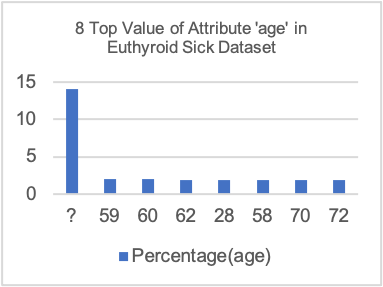
\includegraphics[width=\textwidth]{images/fig10}
        \caption{8 Top Values of Attribute `age' in Euthyroid Sick Dataset}
        \label{fig10}
    \end{minipage}
\end{figure}

In the real world, during the process of acquiring information and data, there will be various causes of data loss and vacancies. There are several options for filling in the missing value. If the missing rate of an attribute is high, this attribute can be deleted directly, so-called listwise deletion \cite{84}. Alternatively, the missing values can be set to specific values calculated on the training set, such as zero, the mean, the median, etc. \cite{85}. For instance, in the Euthyroid Sick Dataset, the missing rate of the attribute `Age' is 14.10\% (466 of 3163). Figure \ref{fig10} shows the 8 top values of this attribute, with the age range of the whole dataset between 1 and 98 years old. During the data cleaning process, this kind of missing value will be replaced with the median of this attribute. Dummy variable adjustment \cite{83} is utilized when the attribute is discrete and has few different values, which can be converted into a dummy variable. For example, in the Thyroid Sick dataset, there are three different values for the gender SEX attribute: `M\footnotemark[11]', `F\footnotemark[12]', `?\footnotemark[13]' (see Figure \ref{fig9}, so this column can be converted into IS\_SEX\_MALE, IS\_SEX\_FEMALE, IS\_SEX\_NA.
\begin{figure}[h]
    \centering 
    \begin{minipage}{0.45\textwidth}
        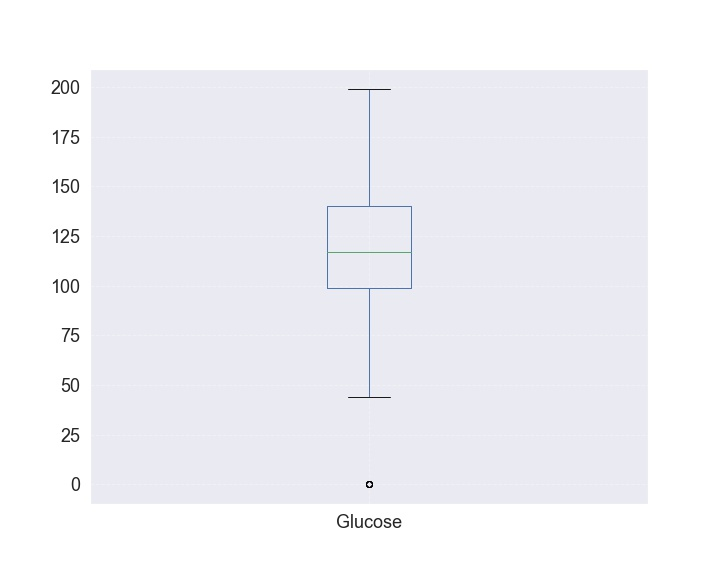
\includegraphics[width=\textwidth]{images/fig11}
        \caption{Box Plot for Attribute `Glucose' in PID Dataset}
        \label{fig11}
    \end{minipage}
    \quad
    \begin{minipage}{0.45\textwidth}
        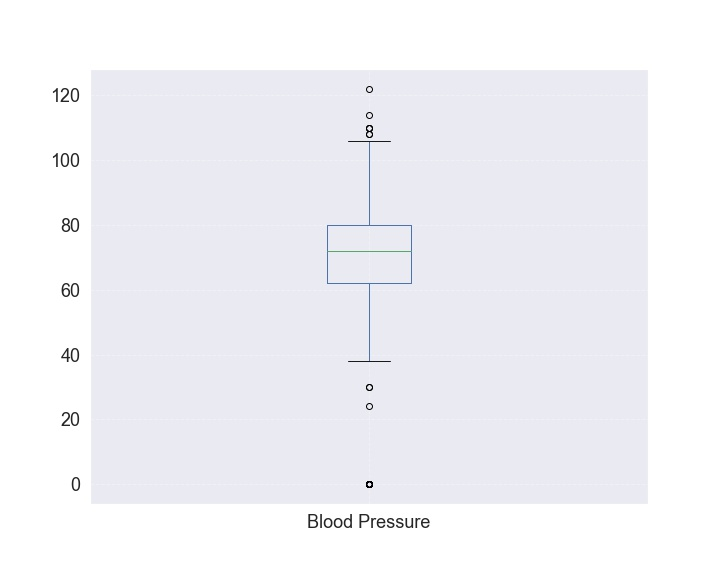
\includegraphics[width=\textwidth]{images/fig12}
        \caption{Box Plot for Attribute `Blood Pressure' in PID Dataset}
        \label{fig12}
    \end{minipage}
\end{figure}

\footnotetext[11]{Male}
\footnotetext[12]{Female}
\footnotetext[13]{Missing Value}

Another kind of data that needs to be cleaned is outlier. Outliers are data points that differ from the rest of the data due to human error, mechanical faults, instrument errors etc. \cite{89}, which is viewed as a normal state of data distribution, and this kind of data outside a specific distribution area or range is also defined as anomalies or abnormalities \cite{88}. One of the visualization methods applied to detect this is box plot using quantiles. Figure \ref{fig11} and Figure \ref{fig12} depict the box plots for the attributes `Blood Pressure' and `Glucose' from the PID dataset. The outliers can be observed clearly in this illustration. There are some instances with an extremely low value for `Blood Pressure' which is rare in the real world. An instance of a 0 `Glucose' can also be viewed as an outlier. Such incorrect data, or data that violates common sense, may lead to an ineffective model. 


There may be variation in the scales of different data features and in the differences between the values \cite{85}. Note the case in the WDBC dataset: the attribute `area\_mean' ranges from 143.5 to 2,501 but the attribute `smoothness\_mean' only ranges from 0.053 to 0.163. This phenomenon may have an impact on the results of data analysis, especially the distance-based algorithms, such as SVM. The data must also be measured to a certain ratio such that they fall into a particular field for detailed analysis \cite{77}. Three normalization procedures \cite{77,78,85} utilized for an attribute $a$ generally are:

Min-Max Normalization\footnotemark[14]\hspace{50pt}$v^{\prime}=\dfrac{v-\min _{a}}{\max _{a}-\min _{a}}\left(n e w_{\max _{a}}-n e w_{\min _{a}}\right)+n e w_{\min _{a}}$
\footnotetext[14]{All the numerical values of the specific numerical attribute $a$ are scaled to a specific range $\left[n e w_{\min _{a}}, n e w_{\max _{a}}\right]$}

Z-score Normalization\footnotemark[15]\hspace{150pt}$v^{\prime}=\dfrac{v-m e a n_{a}}{s t a n d_{-} d e v_{a}}$
\footnotetext[15]{$mean_{a}$ is the sample mean and ${stand\_dev}_{a}$ is the sample standard deviation, which is computed as $\dfrac{1}{n} \sum_{i=1}^{n}\left|v_{i}-mean_{a}\right|$}

Decimal Scaling Normalization\footnotemark[16]\hspace{130pt}$v^{\prime}=\dfrac{v}{10^{j}}$
\footnotetext[16]{where $j$ is the smallest integer such that $n e w_{\max _{a}}<1$}

\begin{table}[h]
    \centering
    \begin{tabular}{|c|c|c|c|c|c|c|}
    \cline{1-2} \cline{4-7}
    \textbf{Raw Number} & \textbf{referral source} & \multirow{6}{*}{$\Longrightarrow$} & \textbf{RSource1} & \textbf{RSource2} & \textbf{RSource3} & \textbf{RSource4} \\ \cline{1-2} \cline{4-7} 
    1                   & SVI                      &                        & 1                 & 0                 & 0                 & 0                 \\ \cline{1-2} \cline{4-7} 
    2                   & STMW                     &                        & 0                 & 0                 & 1                 & 0                 \\ \cline{1-2} \cline{4-7} 
    3                   & SVHD                     &                        & 0                 & 0                 & 0                 & 1                 \\ \cline{1-2} \cline{4-7} 
    4                   & SVHC                     &                        & 0                 & 1                 & 0                 & 0                 \\ \cline{1-2} \cline{4-7} 
    5                   & other                    &                        & 0                 & 0                 & 0                 & 0                 \\ \cline{1-2} \cline{4-7} 
    \end{tabular}
    \caption{Comparison of Before and After One Hot Encoding for Attribute `referral source' in Thyroid Sick Dataset}
    \label{tab7}
\end{table}

Other useful steps are feature encoding \cite{85}, feature selection \cite{87}, dimensionality reduction \cite{85} etc. Since most models have a preference for processing numerical data, handling some text and categorical attributes, feature encoding is a kind of useful data transformation to make data more acceptable as input for models \cite{85}. The attribute `referral source' of thyroid sick dataset contains five values: `SVI', `SVHC', `STMW', `SVHD' and `other'. Table \ref{tab7} shows an example of this attribute before and after transformation. This attribute will be replaced by four new attributes: `RSource1', `RSource2', `RSource3' and `RSource4'. This is also an application of dummy variables adjustment and those new attributes are called dummy attributes. The package Scikit-Learn provides a OneHotEncoder class to transform these kinds of category values into one-hot vectors \cite{85}.

There is no set series of specific data pre-processing methods that can be applied to all data sets, so for different datasets, specific analysis needs to be carried out according to its characteristics \cite{80}.

\subsection{Split of Dataset into Training Set and Testing Set}
For evaluating machine learning algorithms, the Train-Test Split is indispensable, which involves the division of a given dataset into two subset according to a specific ratio. The subset applied to fit the algorithm is called the training set, and the other is referred to as the testing set and is utilized to evaluate the fit algorithm \cite{102}. To be exact, available data with known input vector and target values works on fitting the given model, so that it can predict new instances without class values. In this paper, all the given datasets will be split based on Train:Test = 7:3.

\section{Results on All Models}
\subsection{Overall Comparison}
Tables \ref{tab8}-\ref{tab17} are provided for each separate dataset, listing the performance of each of the models applied in terms of G-mean, F1 and AUCPRC. 

\begin{table}[h]
    \centering
    \begin{tabular}{|p{0.2\textwidth}<{\centering}|p{0.2\textwidth}<{\centering}|p{0.2\textwidth}<{\centering}|p{0.2\textwidth}<{\centering}|}
    \hline
    \multirow{2}{*}{Models} & \multicolumn{3}{c|}{\textbf{Euthyroid Sick}}    \\ \cline{2-4} 
                             & \textbf{G-mean} & \textbf{F1} & \textbf{AUCPRC} \\ \hline
    DDAE                     & 0.880	&0.552	&0.587                \\ \hline
    MWMOTE                   & 0.832	&0.658	&0.616                 \\ \hline
    SMOTE                    & 0.829	&0.667	&0.621                 \\ \hline
    RUSBoost                 & 0.911	&0.725	&0.779                 \\ \hline
    AdaBoost                 & 0.904	&\textbf{0.862}	&\textbf{0.901}                 \\ \hline
    MetaCost                 & 0.935	&0.846	&0.723               \\ \hline
    csDCT                    & 0.960	&0.846	&0.723                 \\ \hline
    CAdaMEC                  & 0.876	&0.831	&0.865                 \\ \hline
    self-paced               & \textbf{0.971}	&0.856	&0.861                 \\ \hline
    IML                      & 0.867	&0.809	&0.836                \\ \hline\hline
    \textbf{Average}         & 0.897	&0.765	&0.751                 \\ \hline
    \end{tabular}
    \caption{Overall Results for Euthyroid Sick Dataset}
    \label{tab8}
\end{table}
%%%%%
\begin{table}[h]
    \centering
    \begin{tabular}{|p{0.2\textwidth}<{\centering}|p{0.2\textwidth}<{\centering}|p{0.2\textwidth}<{\centering}|p{0.2\textwidth}<{\centering}|}
    \hline
    \multirow{2}{*}{Models} & \multicolumn{3}{c|}{\textbf{Thyroid Sick}}    \\ \cline{2-4} 
                             & \textbf{G-mean} & \textbf{F1} & \textbf{AUCPRC} \\ \hline
    DDAE                     & 0.883	&0.506	&0.622               \\ \hline
    MWMOTE                   &0.735	&0.558	&0.342                \\ \hline
    SMOTE                    & 0.694	&0.535	&0.323                \\ \hline
    RUSBoost                 & 0.908	&0.783	&0.805                \\ \hline
    AdaBoost                 & 0.879	&0.828	&0.882                \\ \hline
    MetaCost                 & 0.413	&0.280	&0.342               \\ \hline
    csDCT                    & 0.891	&0.811	&0.700                \\ \hline
    CAdaMEC                  & 0.835	&0.794	&\textbf{0.901}                \\ \hline
    self-paced               & \textbf{0.915}	&\textbf{0.861}	&0.893                 \\ \hline
    IML                      & 0.615	&0.474	&0.335               \\ \hline\hline
    \textbf{Average}         & 0.777	&0.643	&0.615                 \\ \hline
    \end{tabular}
    \caption{Overall Results for Thyroid Sick Dataset}
    \label{tab9}
\end{table}
%%%%
\begin{table}[H]
    \centering
    \renewcommand\arraystretch{0.85}
    \begin{tabular}{|p{0.2\textwidth}<{\centering}|p{0.2\textwidth}<{\centering}|p{0.2\textwidth}<{\centering}|p{0.2\textwidth}<{\centering}|}
    \hline
    \multirow{2}{*}{Models} & \multicolumn{3}{c|}{\textbf{PH1}}    \\ \cline{2-4} 
                             & \textbf{G-mean} & \textbf{F1} & \textbf{AUCPRC} \\ \hline
    DDAE                     & \textbf{0.955}	&0.828	&0.891               \\ \hline
    MWMOTE                   &0.934	&0.781	&0.647                \\ \hline
    SMOTE                    & 0.925	&0.765	&0.630                \\ \hline
    RUSBoost                 & 0.938	&0.868	&0.940                \\ \hline
    AdaBoost                 & 0.940	&\textbf{0.926}	&\textbf{0.963}                \\ \hline
    MetaCost                 & 0.851	&0.774	&0.706               \\ \hline
    csDCT                    & 0.918	&0.837	&0.728                \\ \hline
    CAdaMEC                  & 0.934	&0.913	&0.960               \\ \hline
    self-paced               & 0.936	&0.892	&0.943                 \\ \hline
    IML                      & 0.907	&0.874	&0.925               \\ \hline\hline
    \textbf{Average}         & 0.924	&0.846	&0.833                 \\ \hline
    \end{tabular}
    \vspace{-8pt}
    \caption{Overall Results for PH1 Dataset}
    \label{tab10}
\end{table}
%%%%%
\begin{table}[h]
    \centering
    \begin{tabular}{|p{0.2\textwidth}<{\centering}|p{0.2\textwidth}<{\centering}|p{0.2\textwidth}<{\centering}|p{0.2\textwidth}<{\centering}|}
    \hline
    \multirow{2}{*}{Models} & \multicolumn{3}{c|}{\textbf{PH2}}    \\ \cline{2-4} 
                             & \textbf{G-mean} & \textbf{F1} & \textbf{AUCPRC} \\ \hline
    DDAE                     & 0.986	&0.830	&0.956               \\ \hline
    MWMOTE                   &0.953	&0.664	&0.498               \\ \hline
    SMOTE                    & 0.935	&0.701	&0.546               \\ \hline
    RUSBoost                 &0.996	&0.981	&0.999              \\ \hline
    AdaBoost                 & 0.995	&0.994	&\textbf{1}                \\ \hline
    MetaCost                 & 0.884	&0.794	&0.783               \\ \hline
    csDCT                    & \textbf{0.999}	&\textbf{0.999}	&0.997                \\ \hline
    CAdaMEC                  & 0.995	&0.991	&\textbf{1}               \\ \hline
    self-paced               & \textbf{0.999}	&\textbf{0.999}	&\textbf{1}                 \\ \hline
    IML                      & 0.978	&0.964	&0.999              \\ \hline\hline
    \textbf{Average}         & 0.972	&0.892	&0.878                 \\ \hline
    \end{tabular}
    \vspace{-8pt}
    \caption{Overall Results for PH2 Dataset}
    \label{tab11}
\end{table}
%%%%%
\begin{table}[h]
    \centering
    \renewcommand\arraystretch{0.95} 
    \begin{tabular}{|p{0.2\textwidth}<{\centering}|p{0.2\textwidth}<{\centering}|p{0.2\textwidth}<{\centering}|p{0.2\textwidth}<{\centering}|}
    \hline
    \multirow{2}{*}{Models} & \multicolumn{3}{c|}{\textbf{optdigits}}    \\ \cline{2-4} 
                             & \textbf{G-mean} & \textbf{F1} & \textbf{AUCPRC} \\ \hline
    DDAE                     & \textbf{0.986}	&0.904	&\textbf{0.995}               \\ \hline
    MWMOTE                   &\textbf{0.986}	&0.965	&0.934              \\ \hline
    SMOTE                    & 0.983	&0.968	&0.940               \\ \hline
    RUSBoost                 &0.970	&0.921	&0.971              \\ \hline
    AdaBoost                 & 0.963	&0.955	&0.986               \\ \hline
    MetaCost                 & 0.836	&0.616	&0.490               \\ \hline
    csDCT                    & 0.900	&0.758	&0.637                \\ \hline
    CAdaMEC                  & 0.972	&\textbf{0.985}	&0.992               \\ \hline
    self-paced               & 0.965	&0.946	&0.980                \\ \hline
    IML                      & 0.981	&0.970	&\textbf{0.995}             \\ \hline\hline
    \textbf{Average}         & 0.954	&0.899	&0.892                \\ \hline
    \end{tabular}
    \vspace{-8pt}
    \caption{Overall Results for optdigits Dataset}
    \label{tab12}
\end{table}
%%%%%
\begin{table}[H]
    \centering
    \renewcommand\arraystretch{0.85}
    \begin{tabular}{|p{0.2\textwidth}<{\centering}|p{0.2\textwidth}<{\centering}|p{0.2\textwidth}<{\centering}|p{0.2\textwidth}<{\centering}|}
    \hline
    \multirow{2}{*}{Models} & \multicolumn{3}{c|}{\textbf{MGC}}    \\ \cline{2-4} 
                             & \textbf{G-mean} & \textbf{F1} & \textbf{AUCPRC} \\ \hline
    DDAE                     & \textbf{0.878}	&0.321	&0.324               \\ \hline
    MWMOTE                   &0.798	&0.522	&0.321              \\ \hline
    SMOTE                    & 0.813	&0.539	&0.331               \\ \hline
    RUSBoost                 &0.708	&0.549	&0.513              \\ \hline
    AdaBoost                 & 0.803	&\textbf{0.767}	&\textbf{0.758}               \\ \hline
    MetaCost                 & 0.793	&0.313	&0.208               \\ \hline
    csDCT                    & 0.782	&0.284	&0.141               \\ \hline
    CAdaMEC                  & 0.640	&0.562	&0.627               \\ \hline
    self-paced               & 0.877	&0.516	&0.669                \\ \hline
    IML                      & 0.411	&0.286	&0.270             \\ \hline\hline
    \textbf{Average}         & 0.750	&0.466	&0.416                \\ \hline
    \end{tabular}
    \vspace{-8pt}
    \caption{Overall Results for MGC Dataset}
    \label{tab13}
\end{table}
\vspace{-13pt}
%%%%%
\begin{table}[h]
    \centering
    \begin{tabular}{|p{0.2\textwidth}<{\centering}|p{0.2\textwidth}<{\centering}|p{0.2\textwidth}<{\centering}|p{0.2\textwidth}<{\centering}|}
    \hline
    \multirow{2}{*}{Models} & \multicolumn{3}{c|}{\textbf{WDBC}}    \\ \cline{2-4} 
                             & \textbf{G-mean} & \textbf{F1} & \textbf{AUCPRC} \\ \hline
    DDAE                     & 0.866	&0.831	&0.825               \\ \hline
    MWMOTE                   &0.891	&0.873	&\textbf{0.957}              \\ \hline
    SMOTE                    & \textbf{0.941}	&\textbf{0.937}	&0.945               \\ \hline
    RUSBoost                 &0.911	&0.898	&0.926              \\ \hline
    AdaBoost                 & 0.887	&0.871	&0.832               \\ \hline
    MetaCost                 & 0.887	&0.871	&0.910              \\ \hline
    csDCT                    & 0.907	&0.882	&0.831               \\ \hline
    CAdaMEC                  & 0.891	&0.873	&\textbf{0.957}               \\ \hline
    self-paced               & 0.866	&0.831	&0.825                \\ \hline
    IML                      & 0.893	&0.870	&0.910             \\ \hline\hline
    \textbf{Average}         & 0.894	&0.874	&0.892               \\ \hline
    \end{tabular}
    \vspace{-8pt}
    \caption{Overall Results for WDBC Dataset}
    \label{tab14}
\end{table}
\vspace{-13pt}
%%%%%
\begin{table}[h]
    \centering
    \renewcommand\arraystretch{0.95} 
    \begin{tabular}{|p{0.2\textwidth}<{\centering}|p{0.2\textwidth}<{\centering}|p{0.2\textwidth}<{\centering}|p{0.2\textwidth}<{\centering}|}
    \hline
    \multirow{2}{*}{Models} & \multicolumn{3}{c|}{\textbf{PID}}    \\ \cline{2-4} 
                             & \textbf{G-mean} & \textbf{F1} & \textbf{AUCPRC} \\ \hline
    DDAE                     & 0.712	&0.657	&0.586               \\ \hline
    MWMOTE                   &0.760	&0.780	&0.841             \\ \hline
    SMOTE                    & \textbf{0.807}	&\textbf{0.824}	&\textbf{0.859}               \\ \hline
    RUSBoost                 &0.649	&0.562	&0.642             \\ \hline
    AdaBoost                 & 0.693	&0.671	&0.709               \\ \hline
    MetaCost                 & 0.751	&0.688	&0.734             \\ \hline
    csDCT                    &0.738	&0.671	&0.610              \\ \hline
    CAdaMEC                  & 0.727	&0.658	&0.692               \\ \hline
    self-paced               & 0.640	&0.550	&0.610                \\ \hline
    IML                      & 0.667	&0.587	&0.586             \\ \hline\hline
    \textbf{Average}         & 0.714	&0.665	&0.687               \\ \hline
    \end{tabular}
    \vspace{-8pt}
    \caption{Overall Results for PID Dataset}
    \label{tab15}
\end{table}
%%%%%
\begin{table}[H]
    \centering
    \renewcommand\arraystretch{0.85}
    \begin{tabular}{|p{0.2\textwidth}<{\centering}|p{0.2\textwidth}<{\centering}|p{0.2\textwidth}<{\centering}|p{0.2\textwidth}<{\centering}|}
    \hline
    \multirow{2}{*}{Models} & \multicolumn{3}{c|}{\textbf{Yeast1vs7}}    \\ \cline{2-4} 
                             & \textbf{G-mean} & \textbf{F1} & \textbf{AUCPRC} \\ \hline
    DDAE                     & 0.713	&0.214	&0.257               \\ \hline
    MWMOTE                   &\textbf{0.778}	&0.307	&0.336             \\ \hline
    SMOTE                    &0.775	&0.300	&\textbf{0.468}               \\ \hline
    RUSBoost                 &0.598	& 0.353	&0.304            \\ \hline
    AdaBoost                 & 0.496	&0.333	&0.305              \\ \hline
    MetaCost                 & 0.331	&0.080	&0.083             \\ \hline
    csDCT                    &0	&0	&0.129              \\ \hline
    CAdaMEC                  &0	&0	&0.066              \\ \hline
    self-paced               & 0.740	&0.245	&0.181               \\ \hline
    IML                      & 0.607	&\textbf{0.526}	&0.387             \\ \hline\hline
    \textbf{Average}         & 0.582	&0.237	&0.304               \\ \hline
    \end{tabular}
    \vspace{-8pt}
    \caption{Overall Results for Yeast1vs7 Dataset}
    \label{tab16}
\end{table}
%%%%%
\begin{table}[h]
    \centering
    \vspace{-13pt}
    \begin{tabular}{|p{0.2\textwidth}<{\centering}|p{0.2\textwidth}<{\centering}|p{0.2\textwidth}<{\centering}|p{0.2\textwidth}<{\centering}|}
    \hline
    \multirow{2}{*}{Models} & \multicolumn{3}{c|}{\textbf{Poker8vs6}}    \\ \cline{2-4} 
                             & \textbf{G-mean} & \textbf{F1} & \textbf{AUCPRC} \\ \hline
    DDAE                     &0.622	&0.029	&0.078              \\ \hline
    MWMOTE                   &0.866	&0.857	&0752            \\ \hline
    SMOTE                    &0.999	&0.889	&0.800               \\ \hline
    RUSBoost                 &0.707	&0.667	&0.761            \\ \hline
    AdaBoost                 & \textbf{1}	&\textbf{1}	&\textbf{1}             \\ \hline
    MetaCost                 & 0	&0	&0             \\ \hline
    csDCT                    &0.443	&0.019	&0.009              \\ \hline
    CAdaMEC                  &  0	&0	&0.007              \\ \hline
    self-paced               & 0.613	&0.085	&0.038              \\ \hline
    IML                      & 0.500	&0.400	&0.379             \\ \hline\hline
    \textbf{Average}         & 0.695	&0.523	&0.482               \\ \hline
    \end{tabular}
    \vspace{-8pt}
    \caption{Overall Results for Poker8vs6 Dataset}
    \label{tab17}
\end{table}
\vspace{-20pt}
%%%%%
\begin{table}[h]
    \centering
    \begin{tabular}{|p{0.2\textwidth}<{\centering}|p{0.2\textwidth}<{\centering}|p{0.2\textwidth}<{\centering}|p{0.2\textwidth}<{\centering}|}
    \hline
    \multirow{2}{*}{Models} & \multicolumn{3}{c|}{\textbf{Poker89vs6}}    \\ \cline{2-4} 
                             & \textbf{G-mean} & \textbf{F1} & \textbf{AUCPRC} \\ \hline
    DDAE                     &0.704	&0.051	&0.188             \\ \hline
    MWMOTE                   &0.986	&0.500	&0.750             \\ \hline
    SMOTE                    &0.979	&0.400	&0.750               \\ \hline
    RUSBoost                 &\textbf{1}	&\textbf{1}	&\textbf{1}             \\ \hline
    AdaBoost                 & \textbf{1}	&\textbf{1}	&\textbf{1}             \\ \hline
    MetaCost                 & 0	&0	&0.015             \\ \hline
    csDCT                    &0.495	&0.032	&0.019              \\ \hline
    CAdaMEC                  &   0	&0	&0.014           \\ \hline
    self-paced               & 0.567	&0.036	&0.016              \\ \hline
    IML                      & 0.816	&0.800	&0.848            \\ \hline\hline
    \textbf{Average}         & 0.755	&0.482	&0.559               \\ \hline
    \end{tabular}
    \vspace{-8pt}
    \caption{Overall Results for Poker89vs6 Dataset}
    \label{tab18}
\end{table}
%%%%%
\begin{table}[H]
    \centering
    \renewcommand\arraystretch{0.85} 
    \begin{tabular}{|p{0.2\textwidth}<{\centering}|p{0.2\textwidth}<{\centering}|p{0.2\textwidth}<{\centering}|p{0.2\textwidth}<{\centering}|}
    \hline
    \multirow{2}{*}{Models} & \multicolumn{3}{c|}{\textbf{Cm1}}    \\ \cline{2-4} 
                             & \textbf{G-mean} & \textbf{F1} & \textbf{AUCPRC} \\ \hline
    DDAE                     &0.699	&0.29	&0.214             \\ \hline
    MWMOTE                   &0.679	&0.286	&0.182             \\ \hline
    SMOTE                    &0.715	&0.308	&0.219               \\ \hline
    RUSBoost                 &0.438	&0.25	&0.386            \\ \hline
    AdaBoost                 & \textbf{0.981}	&\textbf{0.970}	&\textbf{0.995}             \\ \hline
    MetaCost                 & 0.744	&0.322	&0.198             \\ \hline
    csDCT                    &0.559	&0.203	&0.158              \\ \hline
    CAdaMEC                  &0.622	&0.237	&0.196             \\ \hline
    self-paced               &0.690	&0.298	&0.262              \\ \hline
    IML                      &0.499	&0.207	&0.137            \\ \hline\hline
    \textbf{Average}         &0.663	&0.337	&0.295              \\ \hline
    \end{tabular}
    \vspace{-8pt}
    \caption{Overall Results for Cm1 Dataset}
    \label{tab19}
\end{table}
\vspace{-23.5pt}
%%%%%
\begin{table}[h]
    \centering
    \begin{tabular}{|p{0.2\textwidth}<{\centering}|p{0.2\textwidth}<{\centering}|p{0.2\textwidth}<{\centering}|p{0.2\textwidth}<{\centering}|}
    \hline
    \multirow{2}{*}{Models} & \multicolumn{3}{c|}{\textbf{Pc1}}    \\ \cline{2-4} 
                             & \textbf{G-mean} & \textbf{F1} & \textbf{AUCPRC} \\ \hline
    DDAE                     &\textbf{0.740}	&0.237	&0.179            \\ \hline
    MWMOTE                   &0.718	&0.226	&0.160            \\ \hline
    SMOTE                    &0.734	&0.244	&0.205               \\ \hline
    RUSBoost                 &0.440	&0.235	&0.214            \\ \hline
    AdaBoost                 & 0.223	&0.091	&0.226            \\ \hline
    MetaCost                 & 0.548	&0.197	&0.109            \\ \hline
    csDCT                    &0.642	&0.185	&0.099              \\ \hline
    CAdaMEC                  &0.673	&0.203	&0.156             \\ \hline
    self-paced               &0.649	&\textbf{0.253}	&\textbf{0.251}              \\ \hline
    IML                      &0.649	&\textbf{0.253}	&\textbf{0.251}          \\ \hline\hline
    \textbf{Average}         &0.602	&\textbf{0.212}	&0.185              \\ \hline
    \end{tabular}
    \vspace{-8pt}
    \caption{Overall Results for Pc1 Dataset}
    \label{tab20}
\end{table}
\vspace{-13pt}
%%%%%
\begin{table}[h]
    \centering
    \begin{tabular}{|p{0.2\textwidth}<{\centering}|p{0.2\textwidth}<{\centering}|p{0.2\textwidth}<{\centering}|p{0.2\textwidth}<{\centering}|}
    \hline
    \multirow{2}{*}{Models} & \multicolumn{3}{c|}{\textbf{Pc4}}    \\ \cline{2-4} 
                             & \textbf{G-mean} & \textbf{F1} & \textbf{AUCPRC} \\ \hline
    DDAE                     &0.756	&0.381	&0.364            \\ \hline
    MWMOTE                   &0.825	&0.497	&0.499            \\ \hline
    SMOTE                    &0.789	&0.460	&0.443               \\ \hline
    RUSBoost                 &0.752	&0.418	&0.413           \\ \hline
    AdaBoost                 &0.823	&\textbf{0.699}	&\textbf{0.714}           \\ \hline
    MetaCost                 &0.790	&0.436	&0.273            \\ \hline
    csDCT                    &0.826	&0.512	&0.364             \\ \hline
    CAdaMEC                  &0.831	&0.475	&0.695             \\ \hline
    self-paced               &\textbf{0.837}	&0.524	&0.453            \\ \hline
    IML                      &0.668	&0.505	&0.416          \\ \hline\hline
    \textbf{Average}         &0.790	&0.491	&0.463             \\ \hline
    \end{tabular}
    \vspace{-8pt}
    \caption{Overall Results for Pc4 Dataset}
    \label{tab22}
\end{table}
%%%%%
\begin{table}[H]
    \centering
    \renewcommand\arraystretch{0.85} 
    \begin{tabular}{|p{0.2\textwidth}<{\centering}|p{0.2\textwidth}<{\centering}|p{0.2\textwidth}<{\centering}|p{0.2\textwidth}<{\centering}|}
    \hline
    \multirow{2}{*}{Models} & \multicolumn{3}{c|}{\textbf{Pc3}}    \\ \cline{2-4} 
                             & \textbf{G-mean} & \textbf{F1} & \textbf{AUCPRC} \\ \hline
    DDAE                     &0.772	&0.440	&0.319            \\ \hline
    MWMOTE                   &\textbf{0.780}&\textbf{0.491}&\textbf{0.401} \\ \hline
    SMOTE                    &0.752	&0.440	&0.376               \\ \hline
    RUSBoost                 &0.452	&0.273	&0.310            \\ \hline
    AdaBoost                 &0.438	&0.289	&0.343            \\ \hline
    MetaCost                 &0.737	&0.432	&0.263            \\ \hline
    csDCT                    &0.719	&0.432	&0.284              \\ \hline
    CAdaMEC                  &0.629	&0.301	&0.336             \\ \hline
    self-paced               &0.719	&0.432	&0.284             \\ \hline
    IML                      &0.418	&0.267	&0.300          \\ \hline\hline
    \textbf{Average}         &0.645	&0.380	&0.322             \\ \hline
    \end{tabular}
    \caption{Overall Results for Pc3 Dataset}
    \label{tab21}
\end{table}
%%%%%

What can be observed from these results is that the G-mean of DDAE is close to or better than the average on most of the datasets. For example, the G-mean value obtained on the MGC is 0.878, while the average value at this time is only 0.750; the G-mean value yielded on Pc1 is 0.740, while the figure for RUSBoost is only 0.44. However, it should be noted that DDAE's F1 and AUCPRC are not satisfactory; they are, lower than the corresponding average values on most of the datasets. In comparison, the two ensemble algorithms, AdaBoost and self-paced Ensemble Classifier, can maintain satisfactory F1, AUCPRC under most circumstances, as well as G-mean,showing that these two algorithms can accurately classify not only a large proportion of minority but also most majority in most cases. For example, AdaBoost has achieved the highest F1 and AUCPRC on datasets such as Euthyroid Sick and PH1, its F1 (0.970) being nearly three times that of MetaCost (0.322), which is the second highest value, on the Cm1 dataset; self-paced Ensemble Classifier has achieved the highest F1 and AUCPRC on Thyroid Sick dataset and PH2 dataset, and its F1 and AUCPRC on Pc1 are twice that of AdaBoost. In addition, the performance of another ensemble algorithm, RUSBoost, is relatively stable, with performance on most datasets being close to the average. 

The stability of cost-sensitive learning models, such as MetaCost, csDCT and CAdaMEC, is not very obvious. CAdaMEC, as well as csDCt, performed well on the optdigits dataset and the Thyroid Sick dataset, but on Yeast1vs7 dataset, its performance is the worst. 

SMOTE and MWMOTE are two sampling models, with a similar performance in most cases except on the Poker8vs6 dataset.

Moreover, the performance of IML fluctuates above and below the average level.Compared with other algorithms, the advantage is not obvious.


%%%%%
\begin{table}[h]
    %\centering
    \begin{tabular}{|p{0.1\textwidth}<{\centering}|p{0.06\textwidth}<{\centering}|p{0.06\textwidth}<{\centering}|p{0.06\textwidth}<{\centering}|p{0.06\textwidth}<{\centering}|p{0.06\textwidth}<{\centering}|p{0.06\textwidth}<{\centering}|p{0.06\textwidth}<{\centering}|p{0.06\textwidth}<{\centering}|p{0.06\textwidth}<{\centering}|p{0.06\textwidth}<{\centering}|}
    \hline
    \multirow{2}{*}{Dataset} & \multicolumn{10}{c|}{\textbf{Recall}}    \\ \cline{2-11} 
                             & \tiny\textbf{DDAE} & \tiny\textbf{MWMOTE} & \tiny\textbf{SMOTE} & \tiny\textbf{RUSBoost} & \tiny\textbf{AdaBoost} & \tiny\textbf{MetaCost} & \tiny\textbf{csDCT} & \tiny\textbf{CAdaMEC} &
                            \tiny\textbf{self-paced} & \tiny\textbf{IML}\\ \hline
    Euthyroid Sick                     &\textbf{0.929}&0.737&0.725&0.888&0.827&0.898&0.867&0.776&0.847&0.763\\ \hline
    Thyroid Sick                   
    &\textbf{0.883}&0.558&0.494&0.844&0.779&0.169&0.805&0.701&0.844&0.383\\ \hline
    PH1                    
    &\textbf{0.956}&0.926&0.913&0.900&0.887&0.741&0.867&0.877&0.887&0.831\\ \hline
    PH2                 
    &0.990&0.946&0.939&0.992&0.990&0.787&\textbf{1}&0.990&0.997&0.931\\ \hline
    % optdigits                 
    % &\textbf{0.994}&0.977&0.971&0.953&0.929&0.759&0.847&0.947&0.935&0.965\\ \hline
    MGC                 
    &\textbf{0.834}&0.651&0.675&0.506&0.675&0.675&0.663&0.410&0.795&0.169\\ \hline
    WDBC                    
    &0.894&0.950&\textbf{0.960}&0.864&0.894&0.818&0.909&0.833&0.864&0.864\\ \hline
    PID                  
    &0.810&0.824&\textbf{0.869}&0.512&0.548&0.774&0.690&0.631&0.524&0.524\\ \hline
    Yeast1vs7               
    &\textbf{0.750}&\textbf{0.750}&\textbf{0.750}&0.375&0.250&0.125&0&\textbf{0.750}&\textbf{0.750}&0.375\\ \hline
    \end{tabular}
    \caption{Recall for for All Models on the Nine Medical Public Datasets}
    \label{tab23}
\end{table}
In order to investigate the ability of theses models mentioned in this paper on positive sample detection, which is important for the field of medical or healthcare, the recall for all these models are presented in Table \ref{tab23}.  

It can be observed that the recall for DDAE performs well on all medical datasets. The recall for self-paced Ensemble Classifier and CAdaMEC can also maintain a relatively stable performance on nearly all the medical datasets.
\begin{table}[h]
    %\centering
    \footnotesize
    \begin{tabular}{|p{0.1\textwidth}<{\centering}|p{0.06\textwidth}<{\centering}|p{0.06\textwidth}<{\centering}|p{0.06\textwidth}<{\centering}|p{0.06\textwidth}<{\centering}|p{0.06\textwidth}<{\centering}|p{0.06\textwidth}<{\centering}|p{0.06\textwidth}<{\centering}|p{0.06\textwidth}<{\centering}|p{0.06\textwidth}<{\centering}|p{0.06\textwidth}<{\centering}|}
    \hline
    \multirow{2}{*}{Dataset} & \multicolumn{10}{c|}{\textbf{Learning Time (in Seconds)}}    \\ \cline{2-11} 
                             & \tiny\textbf{DDAE} & \tiny\textbf{MWMOTE} & \tiny\textbf{SMOTE} & \tiny\textbf{RUSBoost} & \tiny\textbf{AdaBoost} & \tiny\textbf{MetaCost} & \tiny\textbf{csDCT} & \tiny\textbf{CAdaMEC} &
                            \tiny\textbf{self-paced} & \tiny\textbf{IML}\\ \hline
                          
    Euthyroid Sick                     &146.775&0.381&0.224&0.050&0.110&2.426&7.586&0.185&\textbf{0.041}&912.874\\ \hline
    Thyroid Sick                   
    &471.882&1.362&1.711&0.542&1.103&19.91&16.786&0.370&\textbf{0.08}&1680.46\\ \hline
    PH1                    
    &1753.42&0.940&8.006&4.857&2.494&64.927&786.164&1.053&\textbf{0.226}&16627.12\\ \hline
    PH2                 
    &14446.34&115.313&51.917&4.091&5.783&188.748&4513.89&2.770&\textbf{0.302}&46155.96\\ \hline
    optdigits                 
    &637.385&0.983&3.207&0.863&0.976&31.625&166.284&0.372&\textbf{0.07}&5001.329\\ \hline
    MGC                 
    &1472.36&0.845&0.749&0.529&0.679&54.577&31.973&0.231&\textbf{0.065}&9861.933\\ \hline
    WDBC                    
    &13.426&0.950&0.960&\textbf{0.864}&0.894&0.818&0.909&16.117&\textbf{0.864}&8.106\\ \hline
    PID                  
    &17.45&0.381&0.224&0.381&0.478&9.187&15.547&0.089&\textbf{0.029}&27.034\\ \hline
    Yeast1vs7               
    &46.994&0.083&\textbf{0.014}&0.235&0.141&2.411&11.044&0.109&0.036&5.85\\ \hline
    Cm1               
    &54.638&0.069&0.060&\textbf{0.016}&0.106&1.201&36.415&0.086&0.029&10.873\\ \hline
    Pc1               
    &76.463&0.103&0.119&0.244&0.177&3.57&35.073&0.106&\textbf{0.032}&8.702\\ \hline
    Pc3              
    &110.98&0.358&0.053&0.274&0.258&5.388&136.251&0.157&\textbf{0.034}&180.428\\ \hline
    Pc4               
    &97.79&0.399&0.638&0.259&0.208&5.175&65.156&0.118&\textbf{0.038}&156.004\\ \hline
    Poker8vs6               
    &126.932&0.101&\textbf{0.034}&0.185&0.135&4.565&7.267&0.090&0.038&134.869\\ \hline
    Poker89vs6               
    &101.163&0.136&\textbf{0.020}&0.236&0.261&4.617&6.322&0.102&0.029&135.836\\ \hline
    \end{tabular}
    \caption{Learning Time for All Models on the Public Datasets}
    \label{tab24}
\end{table}

\begin{table}[h]
    %\centering
    \footnotesize
    \begin{tabular}{|p{0.1\textwidth}<{\centering}|p{0.06\textwidth}<{\centering}|p{0.06\textwidth}<{\centering}|p{0.06\textwidth}<{\centering}|p{0.06\textwidth}<{\centering}|p{0.06\textwidth}<{\centering}|p{0.06\textwidth}<{\centering}|p{0.06\textwidth}<{\centering}|p{0.06\textwidth}<{\centering}|p{0.06\textwidth}<{\centering}|p{0.06\textwidth}<{\centering}|}
    \hline
    \multirow{2}{*}{Dataset} & \multicolumn{10}{c|}{\textbf{Memory Usage (in MB)}}    \\ \cline{2-11} 
                             & \tiny\textbf{DDAE} & \tiny\textbf{MWMOTE} & \tiny\textbf{SMOTE} & \tiny\textbf{RUSBoost} & \tiny\textbf{AdaBoost} & \tiny\textbf{MetaCost} & \tiny\textbf{csDCT} & \tiny\textbf{CAdaMEC} &
                            \tiny\textbf{self-paced} & \tiny\textbf{IML}\\ \hline
                          
    Euthyroid Sick                     &1.587&0.833&0.388&0.417&\textbf{0.342}&0.418&1.449&0.369&0.399&0.977\\ \hline
    Thyroid Sick                   
    &1.978&0.425&0.362&0.403&\textbf{0.344}&0.41&0.956&0.364&0.354&0.481\\ \hline
    PH1                    
    &1.964&0.428&0.356&0.391&\textbf{0.338}&0.4&1.149&0.357&0.348&0.592\\ \hline
    PH2                 
    &1.986&0.817&0.369&0.417&\textbf{0.350}&0.417&1.523&0.351&0.366&0.607\\ \hline
    optdigits                 
    &1.677&0.416&0.439&0.344&\textbf{0.330}&0.394&0.813&0.336&0.336&0.413\\ \hline
    MGC                 
    &1.996&0.822&0.885&0.425&\textbf{0.347}&0.762&1.055&0.376&0.353&0.457\\ \hline
    WDBC                    
    &1.609&0.549&0.451&0.677&0.390&\textbf{0.388}&1.414&0.725&0.447&0.619\\ \hline
    PID                  
    &0.707&0.457&0.450&0.355&\textbf{0.338}&0.383&0.810&0.343&0.346&0.426\\ \hline
    Yeast1vs7               
    &0.430&0.438&0.428&0.354&\textbf{0.334}&0.396&0.781&0.342&0.358&0.504\\ \hline
    Cm1               
    &1.499&0.614&0.515&0.399&\textbf{0.343}&0.41&0.829&0.366&0.358&0.437\\ \hline
    Pc1               
    &1.966&0.549&0.451&0.677&\textbf{0.390}&0.388&1.41&0.725&0.447&0.619\\ \hline
    Pc3              
    &1.503&0.530&0.458&0.793&\textbf{0.361}&0.417&1.305&0.372&0.381&0.612\\ \hline
    Pc4               
    &1.007&0.474&0.429&0.366&\textbf{0.342}&0.387&0.808&0.348&0.348&0.434\\ \hline
    Poker8vs6               
    &1.510&0.525&0.464&0.392&\textbf{0.344}&0.408&0.911&0.367&0.365&0.435\\ \hline
    Poker89vs6               
    &0.638&0.404&0.418&0.36&\textbf{0.336}&0.395&0.836&0.346&0.346&0.426\\ \hline
    \end{tabular}
    \caption{Memory Usage for All Models on the Public Datasets}
    \label{tab27}
\end{table}

Table \ref{tab24} shows the learning time achieved by each algorithm on different datasets. It can be seen that IML and DDAE yields the two most longest learning time compared to the other algorithms. Self-paced Ensemble Classifier performs fairly well in terms of learning time with most of the values ranging in (0, 0.1). Considering the characteristics of the datasets described in section 4.1.1, it can be illustrated that, the larger the dataset is, the longer the learning time required for the algorithms. 


Table \ref{tab27} illustrates the memory usage of each algorithm. It can be observed that the memory usage for each algorithm are similar, even the algorithms are processing the different dataset, and there is no obvious relation between the memory usage and the size of the dataset. Among all these algorithms, AdaBoost and self-paced Ensemble Classifier are two algorithms with the lowest memory usage.

\subsection{Impact of Imbalanced Ratio}
First, to analyze the influence of IR on the model, eight identically-sized sub-datasets with different imbalance ratios (IRs) were used in the experiment. They were IR=10, 20, 30, 40, 50, 60, 70, 80 and 90. The x-axis for Figures \ref{fig13}-\ref{fig17} is IR.
\begin{figure}[h]
    \centering 
    \begin{minipage}{0.45\textwidth}
        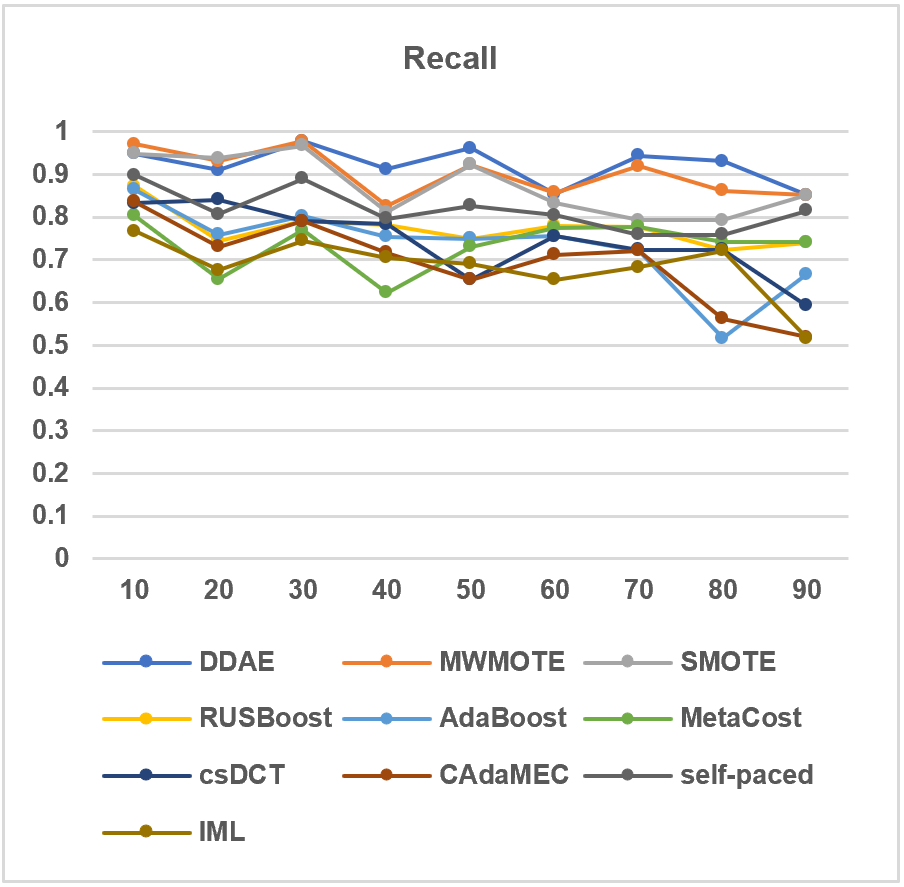
\includegraphics[width=\textwidth]{images/fig13}
        \caption{Recall: Impact of Imbalance Ratio}
        \label{fig13}
    \end{minipage}
    \quad
    \begin{minipage}{0.45\textwidth}
        \vspace{9.5pt}
        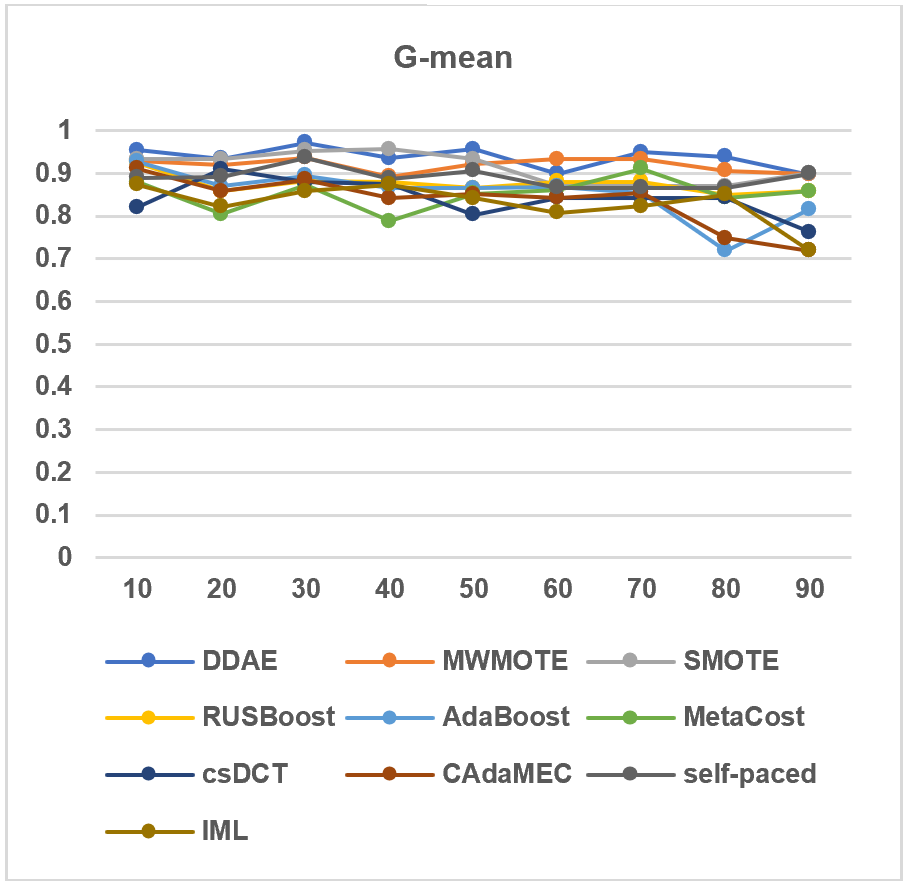
\includegraphics[width=\textwidth]{images/fig15}
        \caption{G-mean: Impact of Imbalance Ratio}
        \label{fig15}
    \end{minipage}
\end{figure}

Figure \ref{fig13} illustrates the trend of recall of all algorithms as the IR increases. Clearly, this metric stays stable on DDAE most of the time, and DDAE keeps the recall between 0.9 and 0.95. MWMOTE, SMOTE, cost-sensitive Decision Tree, CAdaMEC, self-paced Ensemble Classifier and IML show a downward trend. Among these, the recall of MWMOTE, SMOTE and self-paced Ensemble Classifier decreased slightly as the class distribution became more imbalanced, with the highest and lowest values for MWMOTE, SMOTE, AdaBoost and self-paced Ensemble Classifier being 0.978(IR=30) and 0.852 (IR=90), 0.967 (IR=30) and 0.793 (IR=80), 0.865 (IR=10) and 0.517 (IR=80), 0.898 (IR=10) and 0.795 (IR=80), respectively. The figures for recall of the other four ``decreasing'' algorithms drop significantly, from 0.841 (IR=20) to 0.593 (IR=90) for csDCT, from 0.836 (IR=10) to 0.519 (IR=90) for CAdaMEC, and from 0.767 (IR=10) to 0.517 (IR=90) for IML. In addition, no obvious correlation between recall and the changes in IR can be seen through the curves of RUSBoost and MetaCost. All of them show a slight fluctuation in this process.

% The impact of IR on the precision of these models can be viewed in Figure \ref{fig14}. More than half of all models show a decrease as the IR climbs up, including DDAE, MWMOTE, SMOTE, csDCT and self-paced Ensemble Classifier. The difference between maximum and minimum for these models is 0.548, 0.374, 0.416, 0.577 and 0.442, respectively. In contrast, the figure for RUSBoost goes up after IR is greater than 30. Even though the curves of CAdaMEC and MetaCost are fluctuant, they still decrease slightly. Moreover, the precision of IML and AdaBoost maintain stability during the whole experiment, with the precision generally above 0.9 for both of the models.

Notably, the G-mean of almost all the models remain nearly stable with the exception of MetaCost. All of the models still retain a high value for G-mean even when the IR is 70 or 80. It can be observed from Figure \ref{fig15} that some of models performs better (or similarly) when the IR is 70 compared to the IR is 10, including DDAE, MWMOTE, SMOTE, RUSBoost, AdaBoost, MetaCost, self-paced Ensemble Classifier, IML and csDCT. 




% RUSBoost and AdaBoost show a decrease when the IR is greater than 80 and 70, respectively. 


% \begin{figure}[h]
%     \centering 
%     % \begin{minipage}{0.31\textwidth}
%     %     \centering
%     %     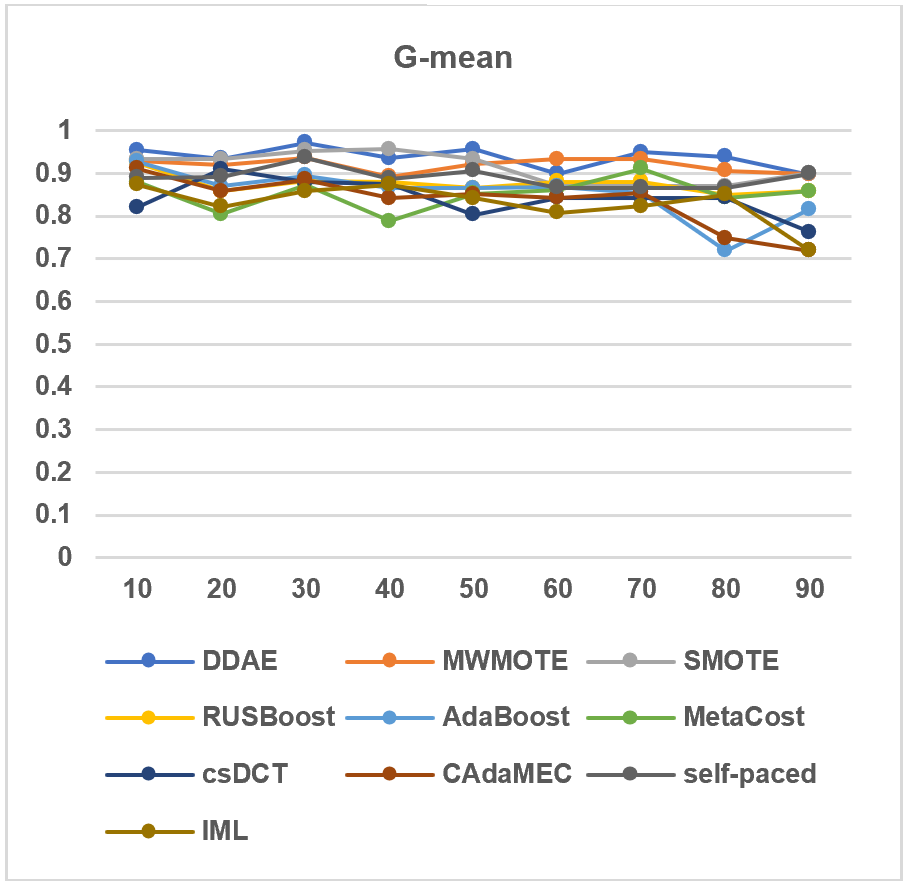
\includegraphics[width=\textwidth]{images/fig15}
%     %     \caption{G-mean: Impact of Imbalance Ratio}
%     %     \label{fig15}
%     % \end{minipage}
%     % \hspace{5pt}
%     \begin{minipage}{0.45\textwidth}
%         \centering
%         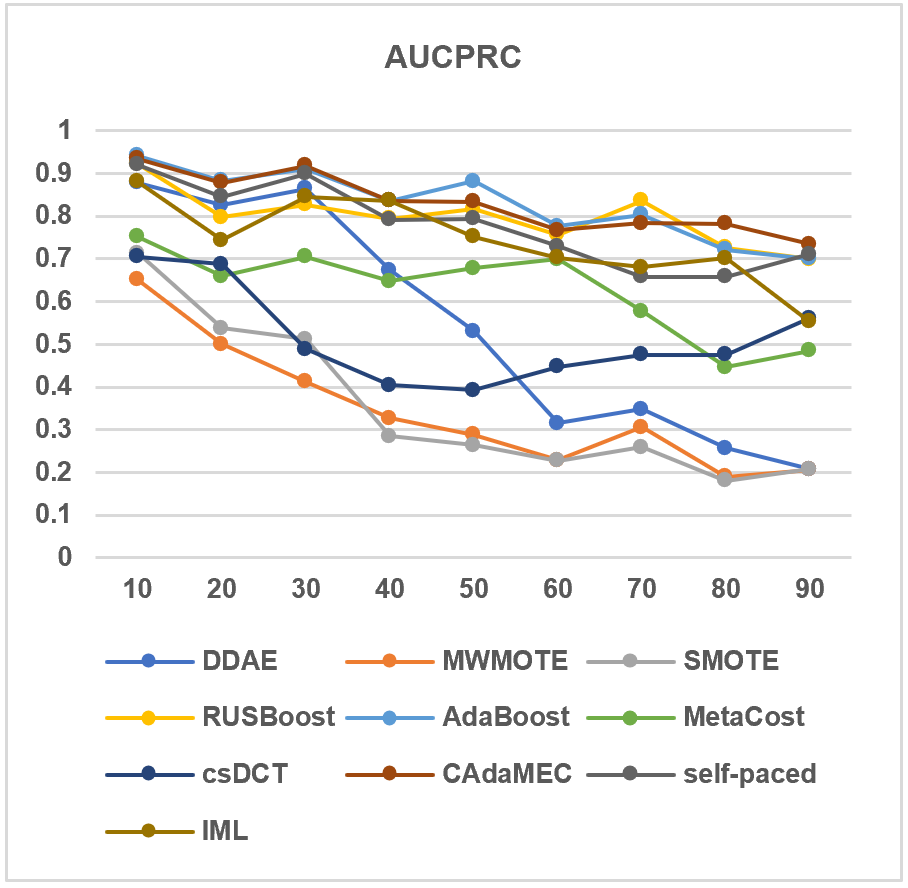
\includegraphics[width=\textwidth]{images/fig16}
%         \caption{AUCPRC: Impact of Imbalance Ratio}
%         \label{fig16}
%     \end{minipage}
%     \quad
%     \begin{minipage}{0.45\textwidth}
%         \vspace{9.5pt}
%         % \centering
%         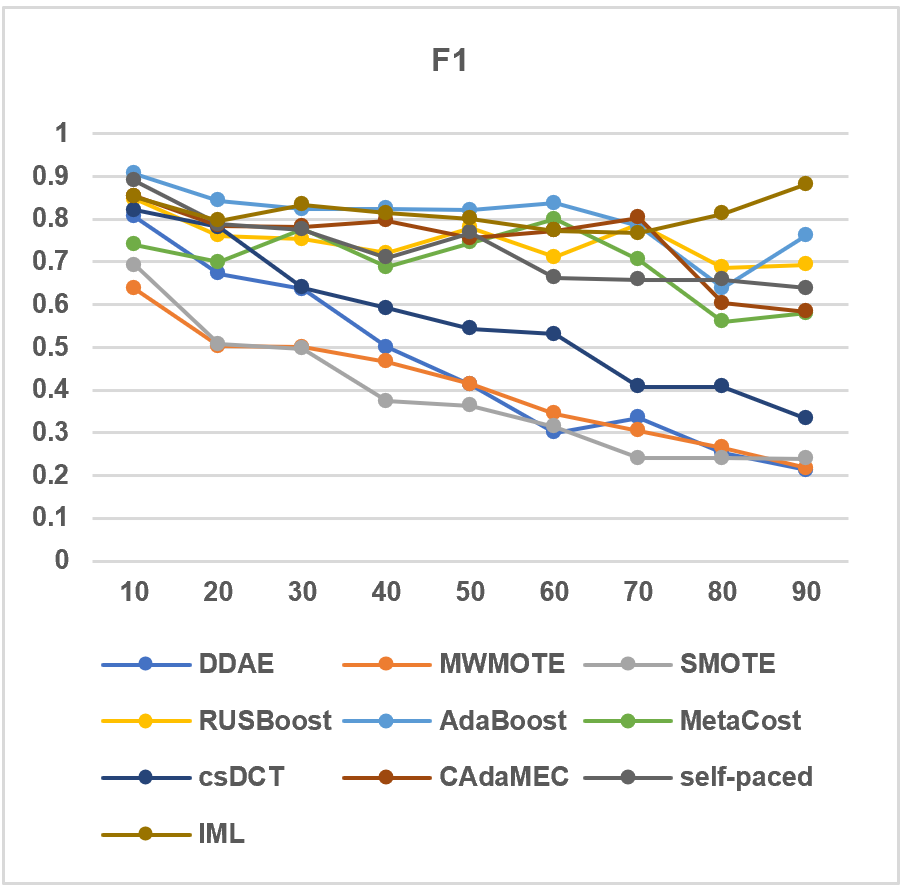
\includegraphics[width=\textwidth]{images/fig17}
%         \caption{F1: Impact of Imbalance Ratio}
%         \label{fig17}
%     \end{minipage}
% \end{figure}
\begin{figure}[h]
    \centering 
    \begin{minipage}[t]{0.45\textwidth}
        \vspace{0pt}
        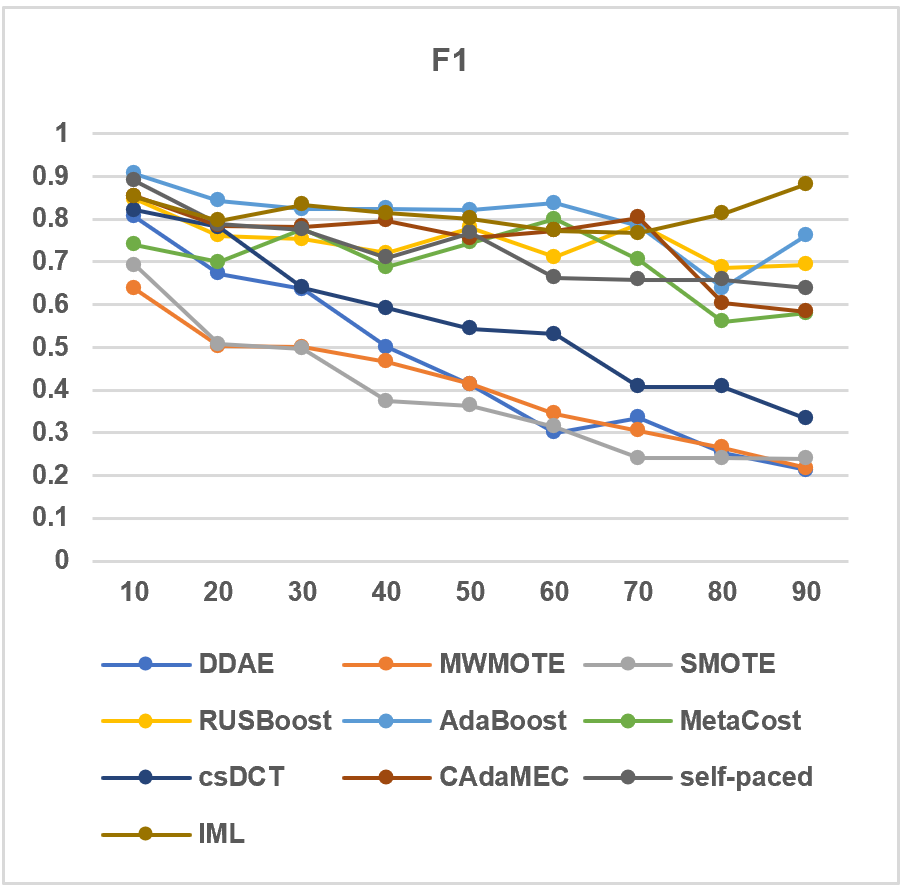
\includegraphics[width=\textwidth]{images/fig17}
        \caption{F1: Impact of Imbalance Ratio}
        \label{fig17}
    \end{minipage}
    \quad
    \begin{minipage}[t]{0.45\textwidth}
        \vspace{0pt}
        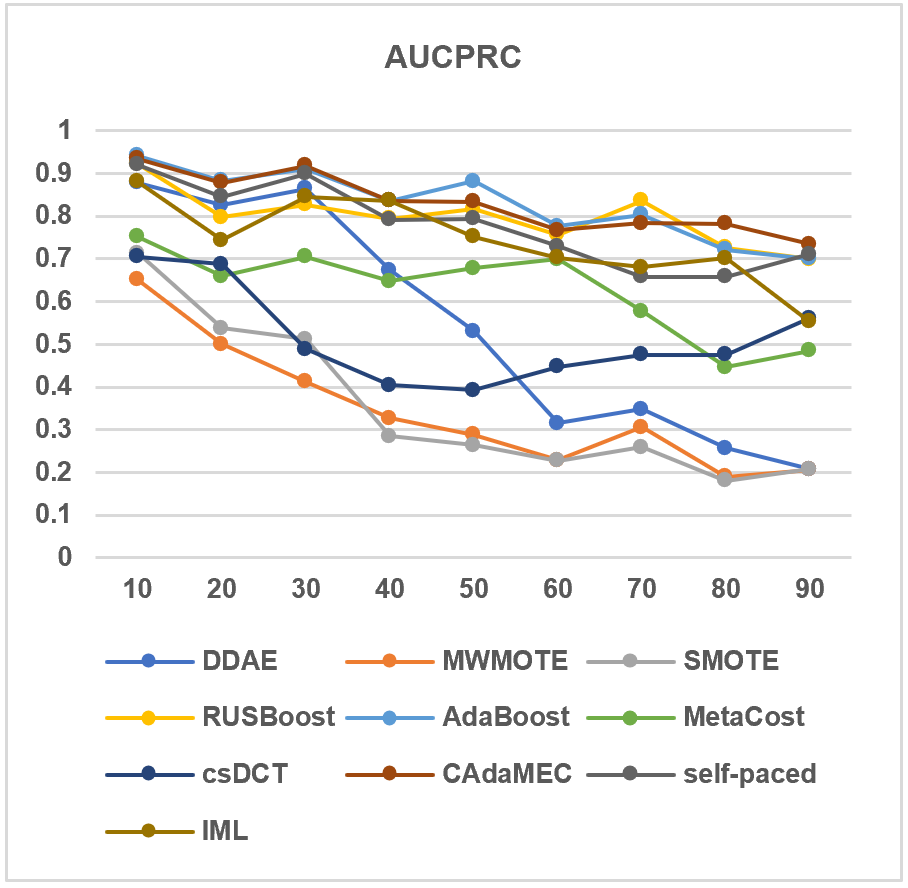
\includegraphics[width=\textwidth]{images/fig16}
        \caption{AUCPRC: Impact of Imbalance Ratio}
        \label{fig16}
    \end{minipage}
\end{figure}

F1 is the evaluation metric which takes both recall and precision into account, which means that if the trend of recall for one specific model maintain stability with only a slight decrease/increase, the changes in F1 will be similar to those in precision. According to the above description of the changes in recall, the trends for F1 of SMOTE, MWMOTE, DDAE, csDCT can be compared with those for their precision, which can be observed from Figure \ref{fig17}. The value of F1 for MetaCost and AdaBoost decrease slightly during the process. In contrast, as the performance of other models shows degradation to some degree, the figures for IML, RUSBoost and self-paced Ensemble Classifier stay almost stable, but the former increases slightly after IR is greater than 70 and the latter drops to a small degree. AUCPRC is another evaluation metric which considers recall and precision at the same time. According to Figure \ref{fig16}, the AUCPRCs for DDAE, MWMOTE, SMOTE, CAdaMEC and IML decrease as the IR increases. The figure for MetaCost fluctuates significantly but is still showing a decrease. The AUCPRCs for AdaBoost, RUSBoost and self-paced Ensemble Classifier are all on a slightly downward trend. Moreover, csDCT preforms differently on AUCPRC from other models, the figure for these two models climbing when the IR varies from 50 to 90. 

\subsection{Impact of the Size of Datasets}



% \begin{figure}[h]
%     \centering 
%     \begin{minipage}{0.31\textwidth}
%         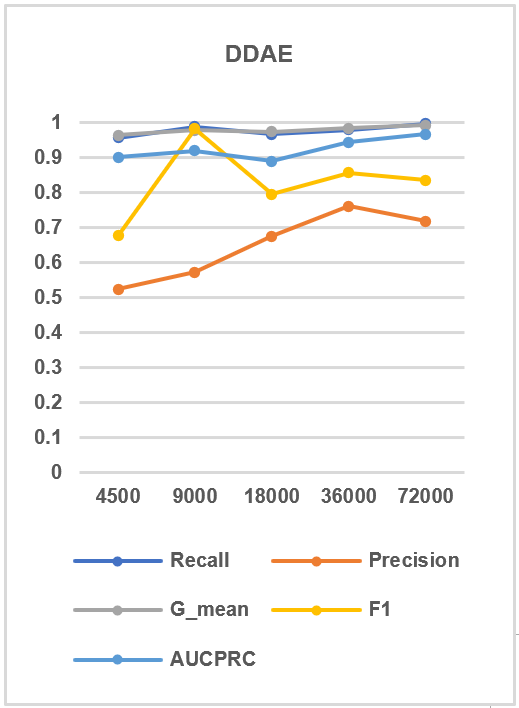
\includegraphics[width=\textwidth]{images/fig18}
%         \caption{DDAE: Impact of the Size of Dataset}
%         \label{fig18}
%     \end{minipage}
%     \begin{minipage}{0.31\textwidth}
%         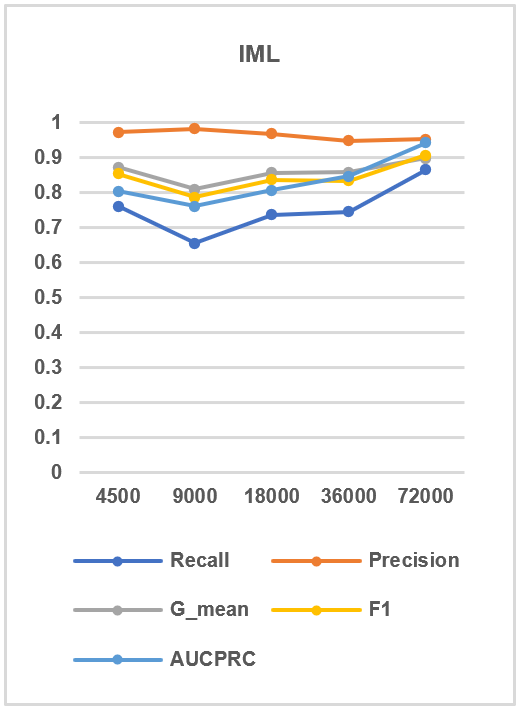
\includegraphics[width=\textwidth]{images/fig19}
%         \caption{IML: Impact of the Size of Dataset}
%         \label{fig19}
%     \end{minipage}
%     \begin{minipage}{0.31\textwidth}
%         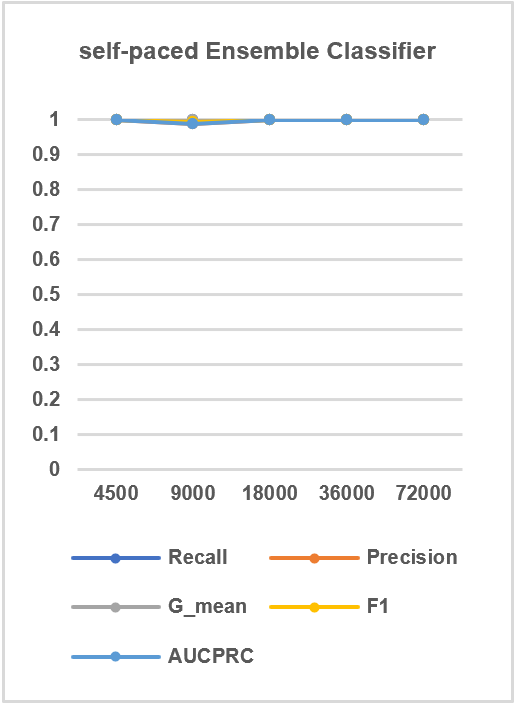
\includegraphics[width=\textwidth]{images/fig20}
%         \caption{self-paced: Impact of the Size of Dataset}
%         \label{fig20}
%     \end{minipage}

%     \begin{minipage}{0.31\textwidth}
%         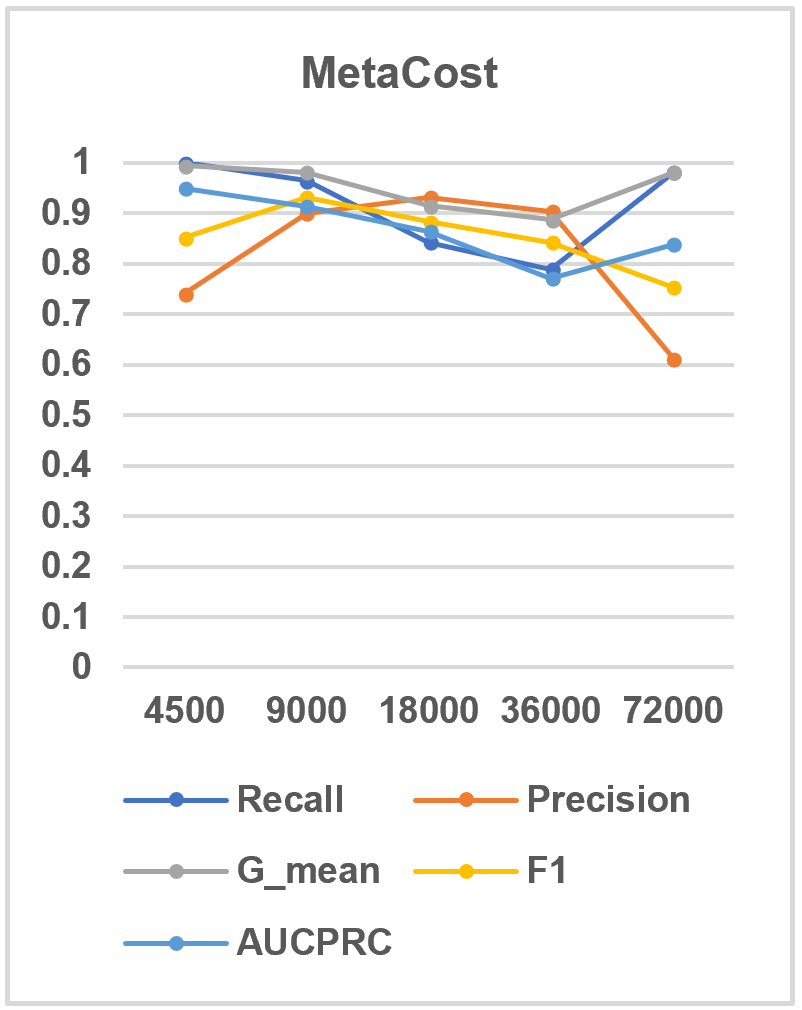
\includegraphics[width=\textwidth]{images/fig21}
%         \caption{MetaCost: Impact of the Size of Dataset}
%         \label{fig21}
%     \end{minipage}
%     \begin{minipage}{0.31\textwidth}
%         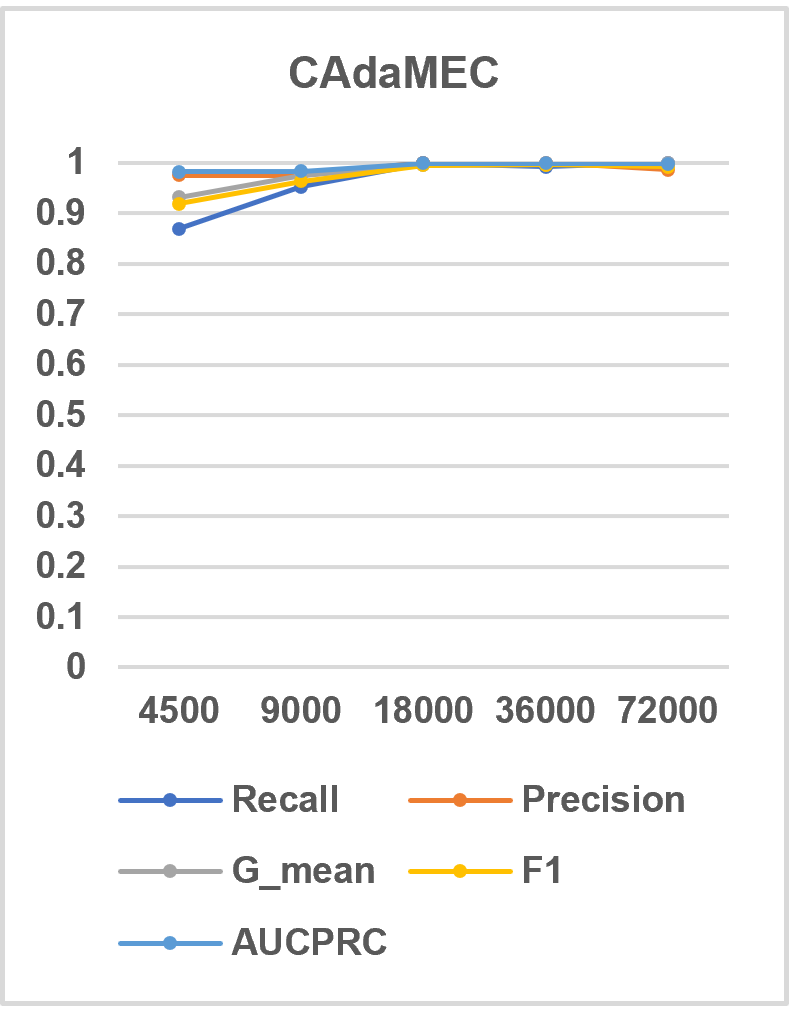
\includegraphics[width=\textwidth]{images/fig22}
%         \caption{CAdaMEC: Impact of the Size of Dataset}
%         \label{fig22}
%     \end{minipage}
%     \begin{minipage}{0.31\textwidth}
%         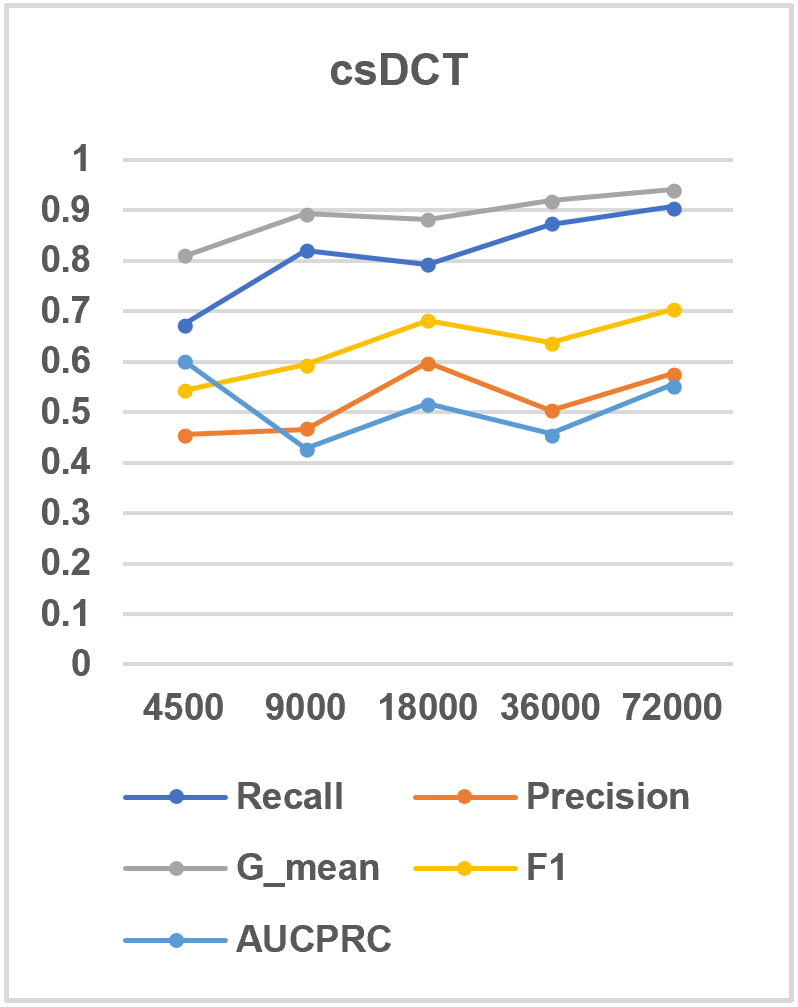
\includegraphics[width=\textwidth]{images/fig23}
%         \caption{csDCT: Impact of the Size of Dataset}
%         \label{fig23}
%     \end{minipage}

%     \begin{minipage}{0.31\textwidth}
%         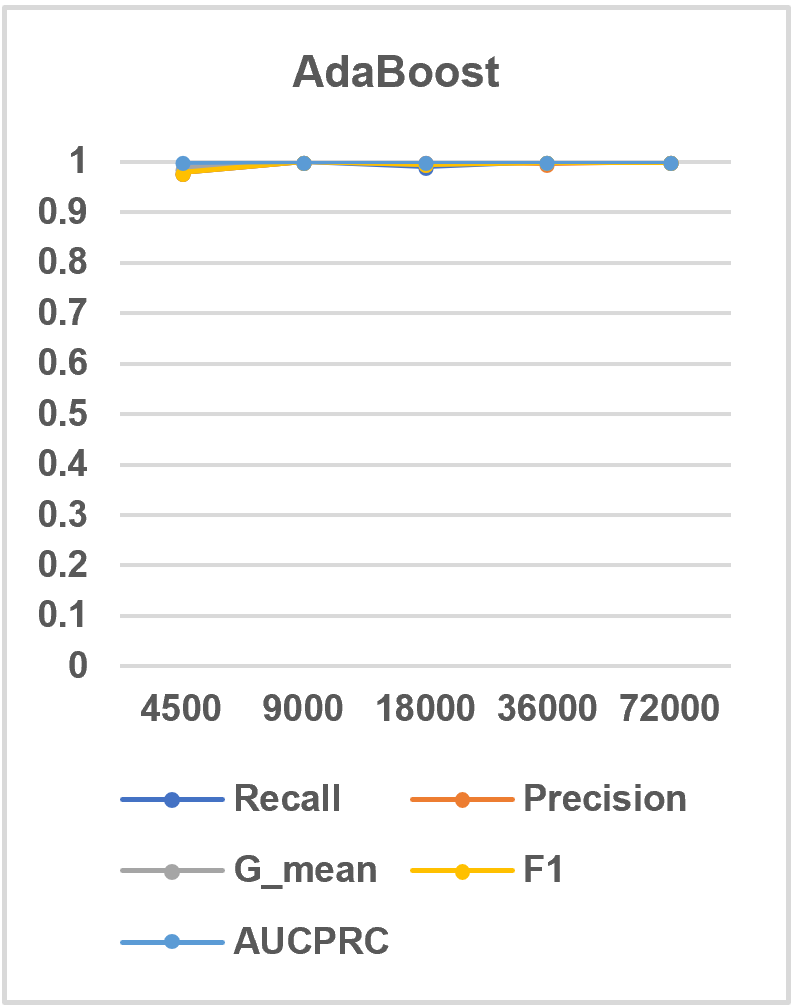
\includegraphics[width=\textwidth]{images/fig24}
%         \caption{AdaBoost: Impact of the Size of Dataset}
%         \label{fig24}
%     \end{minipage}
%     \begin{minipage}{0.31\textwidth}
%         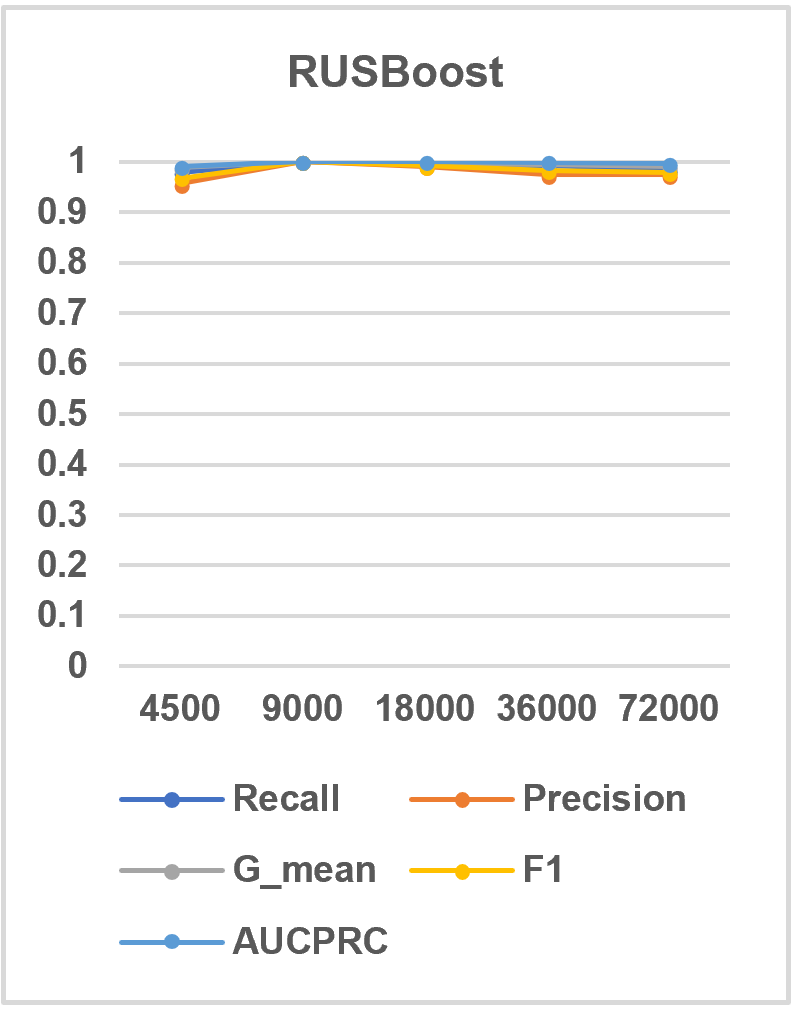
\includegraphics[width=\textwidth]{images/fig25}
%         \caption{RUSBoost: Impact of the Size of Dataset}
%         \label{fig25}
%     \end{minipage}
%     \begin{minipage}{0.31\textwidth}
%         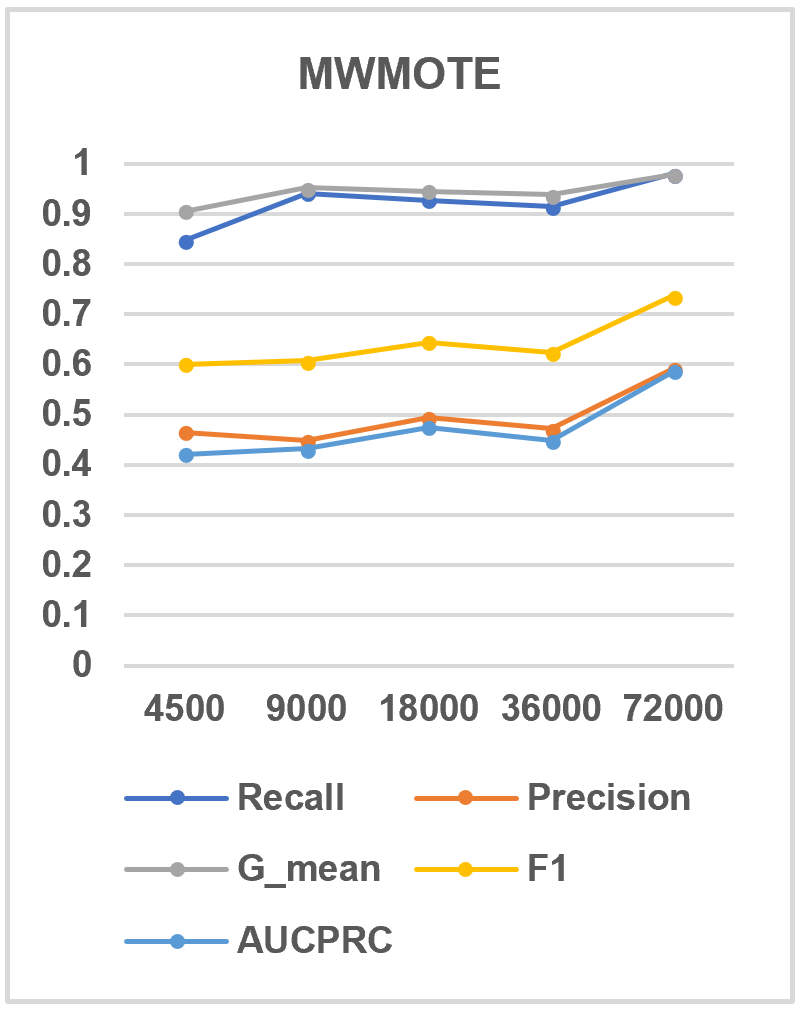
\includegraphics[width=\textwidth]{images/fig26}
%         \caption{MWMOTE: Impact of the Size of Dataset}
%         \label{fig26}
%     \end{minipage}

%     \begin{minipage}{0.31\textwidth}
%         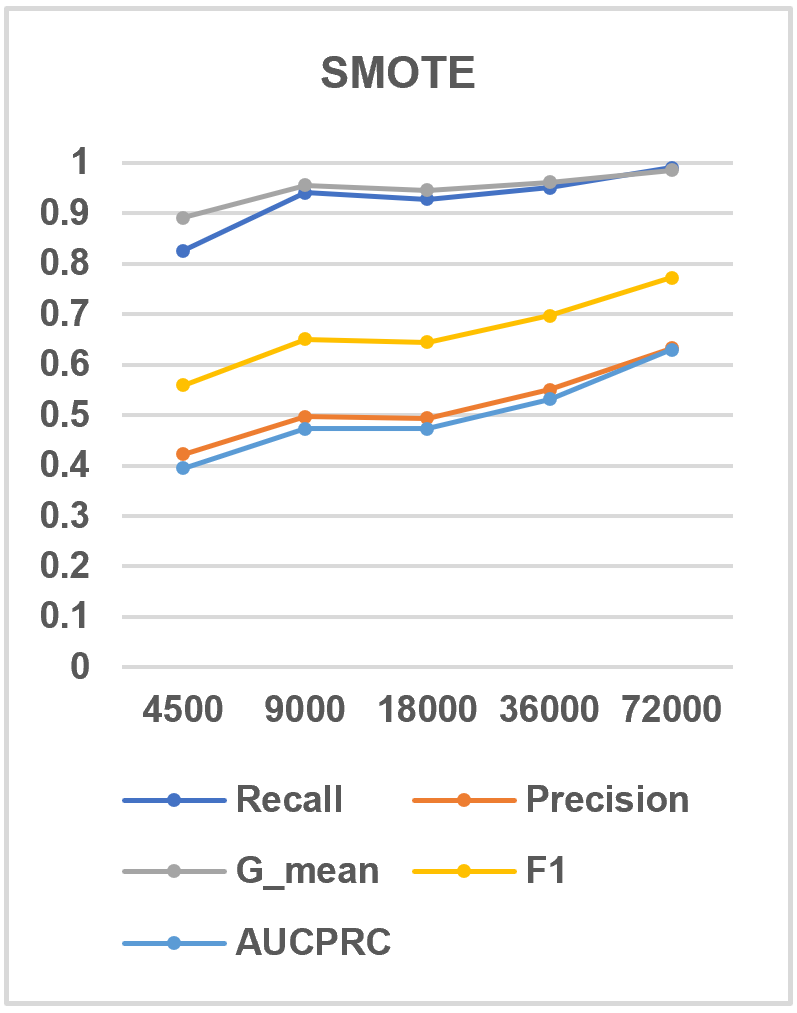
\includegraphics[width=\textwidth]{images/fig27}
%         \caption{IML: Impact of the Size of Dataset}
%         \label{fig27}
%     \end{minipage}
% \end{figure}

\begin{figure}[H]
    \centering 
    \begin{minipage}{0.31\textwidth}
        \centering
        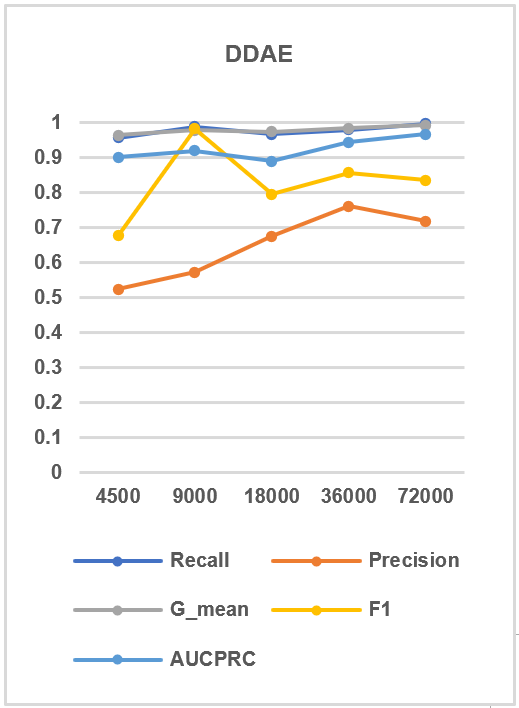
\includegraphics[width=0.8\textwidth]{images/fig18}
        \caption{DDAE: Impact of the Size of Dataset}
        \label{fig18}
    \end{minipage}
    \hspace{5pt}
    \begin{minipage}{0.31\textwidth}
        \centering
        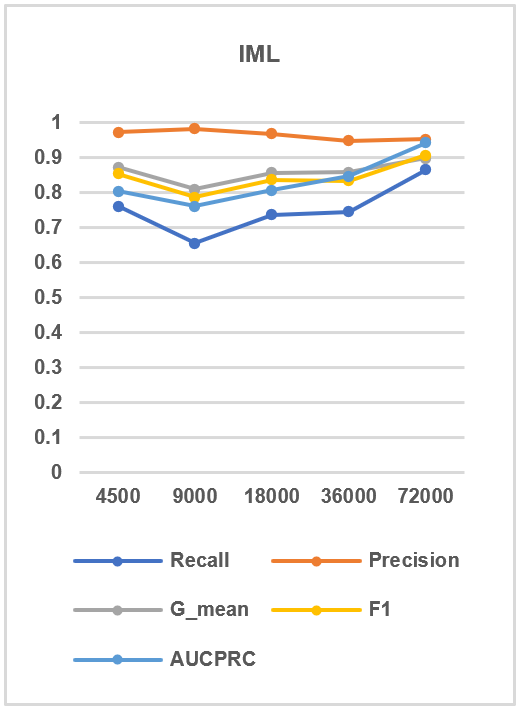
\includegraphics[width=0.8\textwidth]{images/fig19}
        \caption{IML: Impact of the Size of Dataset}
        \label{fig19}
    \end{minipage}
    \hspace{5pt}
    \begin{minipage}{0.31\textwidth}
        \centering
        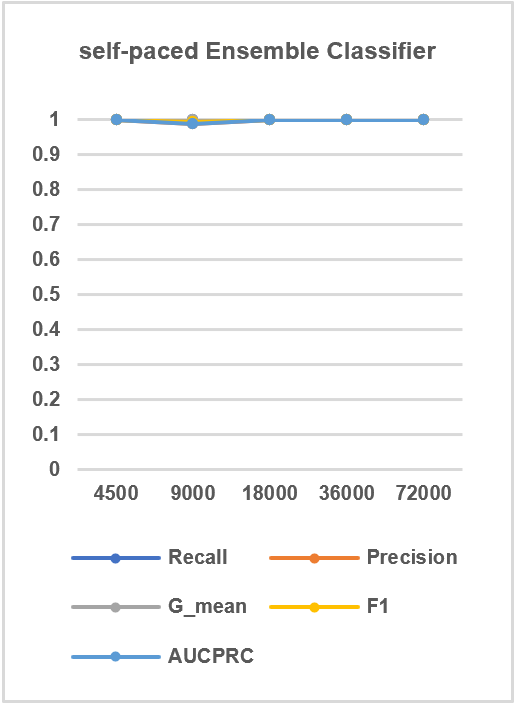
\includegraphics[width=0.8\textwidth]{images/fig20}
        \caption{self-paced: Impact of the Size of Dataset}
        \label{fig20}
    \end{minipage}
\end{figure}
\vspace{-10pt}

\begin{figure}[h]
    \centering 
    \begin{minipage}{0.31\textwidth}
        \centering
        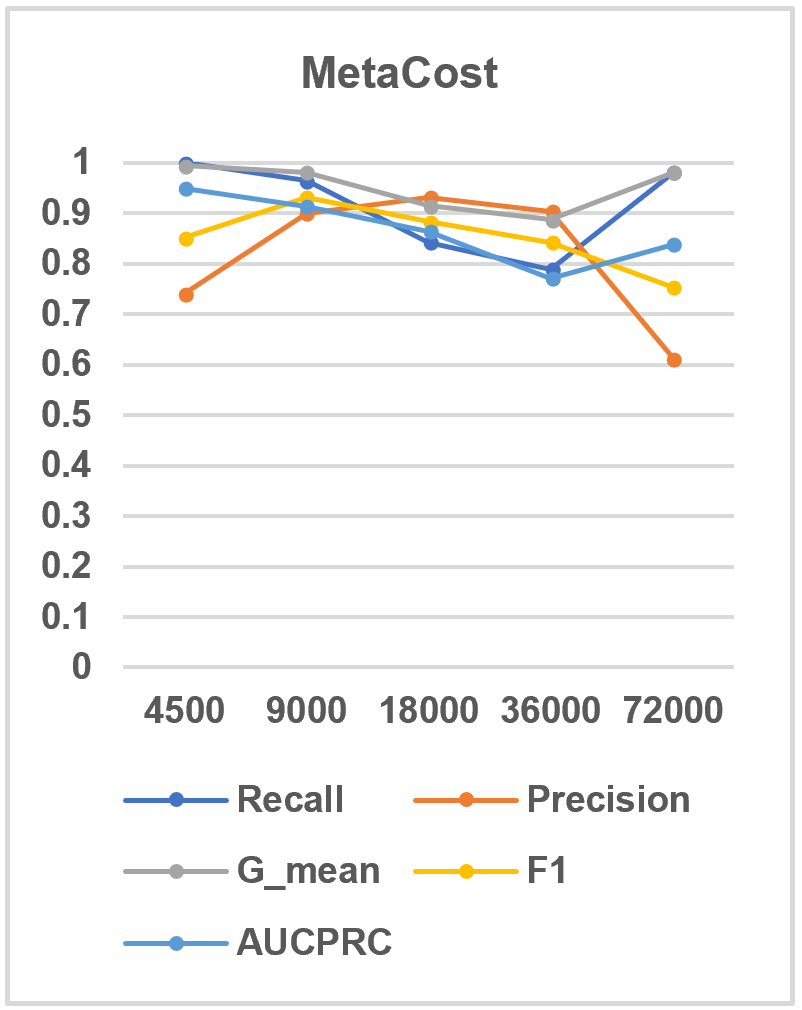
\includegraphics[width=0.8\textwidth]{images/fig21}
        \caption{MetaCost: Impact of the Size of Dataset}
        \label{fig21}
    \end{minipage}
    \hspace{5pt}
    \begin{minipage}{0.31\textwidth}
        \centering
        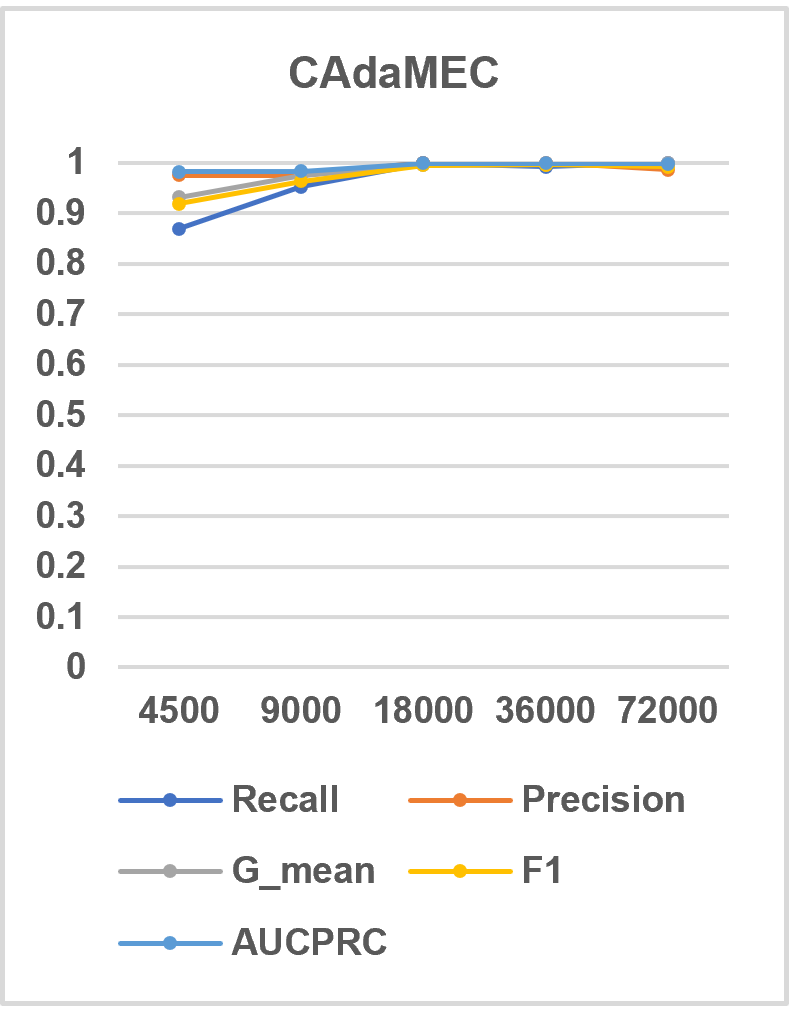
\includegraphics[width=0.8\textwidth]{images/fig22}
        \caption{CAdaMEC: Impact of the Size of Dataset}
        \label{fig22}
    \end{minipage}
    \hspace{5pt}
    \begin{minipage}{0.31\textwidth}
        \centering
        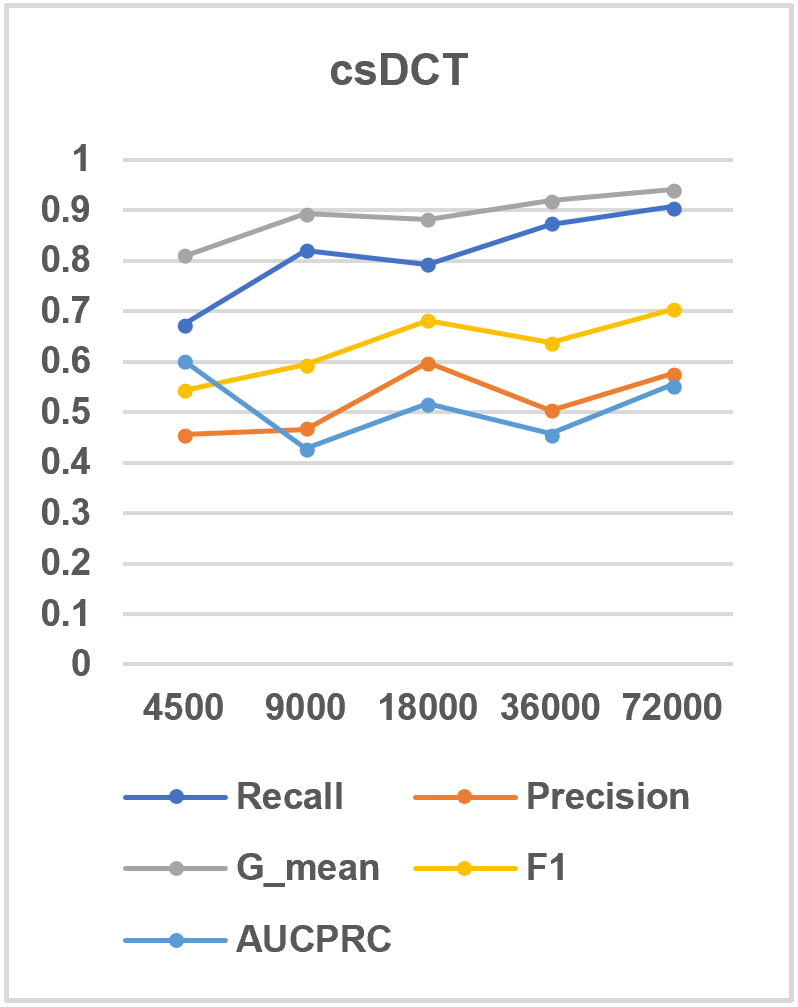
\includegraphics[width=0.8\textwidth]{images/fig23}
        \caption{csDCT: Impact of the Size of Dataset}
        \label{fig23}
    \end{minipage}
\end{figure}
\vspace{-10pt}

\begin{figure}[H]
    \centering 
    \begin{minipage}{0.31\textwidth}
        \centering
        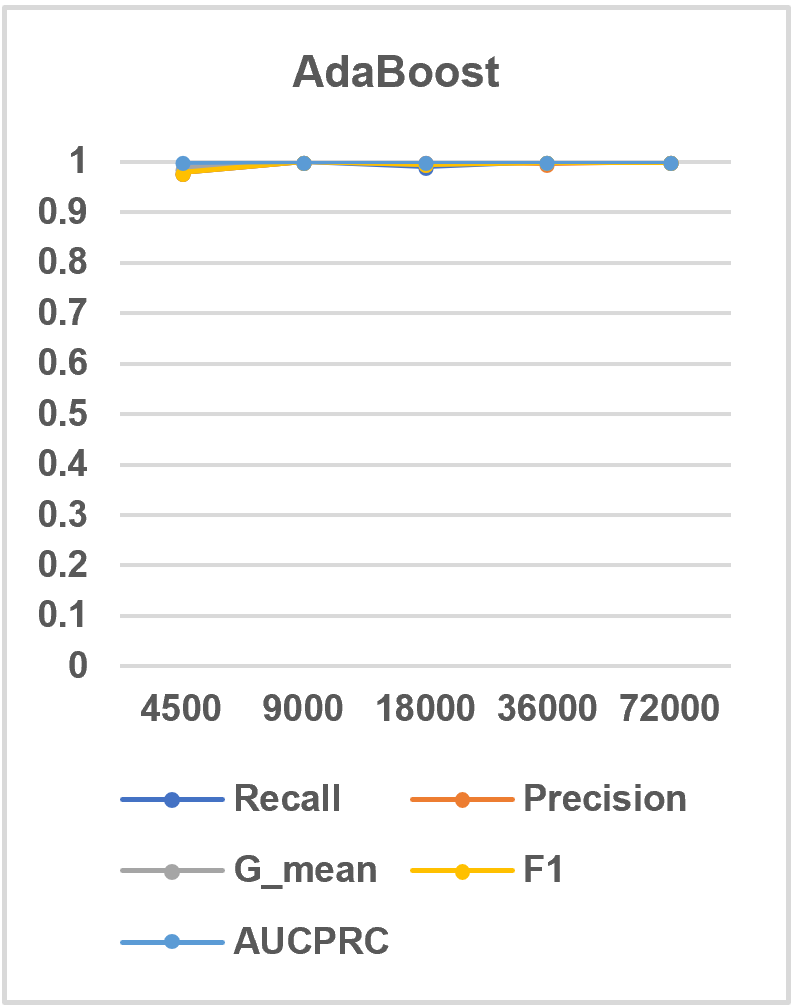
\includegraphics[width=0.8\textwidth]{images/fig24}
        \caption{AdaBoost: Impact of the Size of Dataset}
        \label{fig24}
    \end{minipage}
    \hspace{5pt}
    \begin{minipage}{0.31\textwidth}
        \centering
        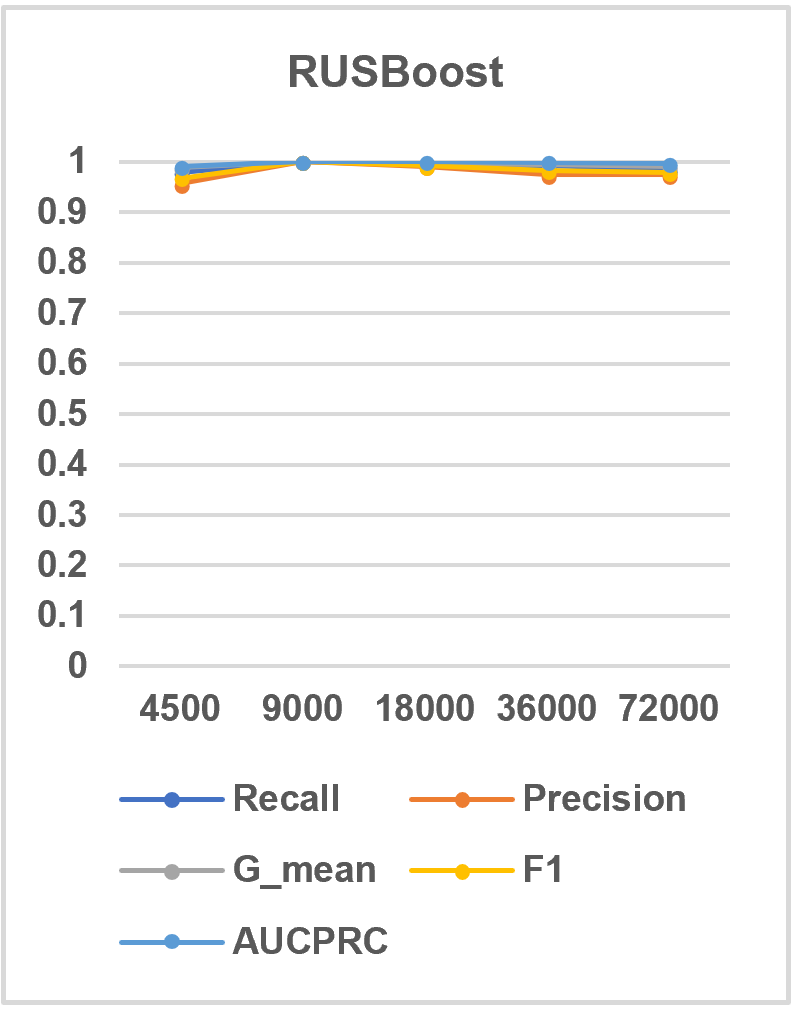
\includegraphics[width=0.8\textwidth]{images/fig25}
        \caption{RUSBoost: Impact of the Size of Dataset}
        \label{fig25}
    \end{minipage}
    \hspace{5pt}
    \begin{minipage}{0.31\textwidth}
        \centering
        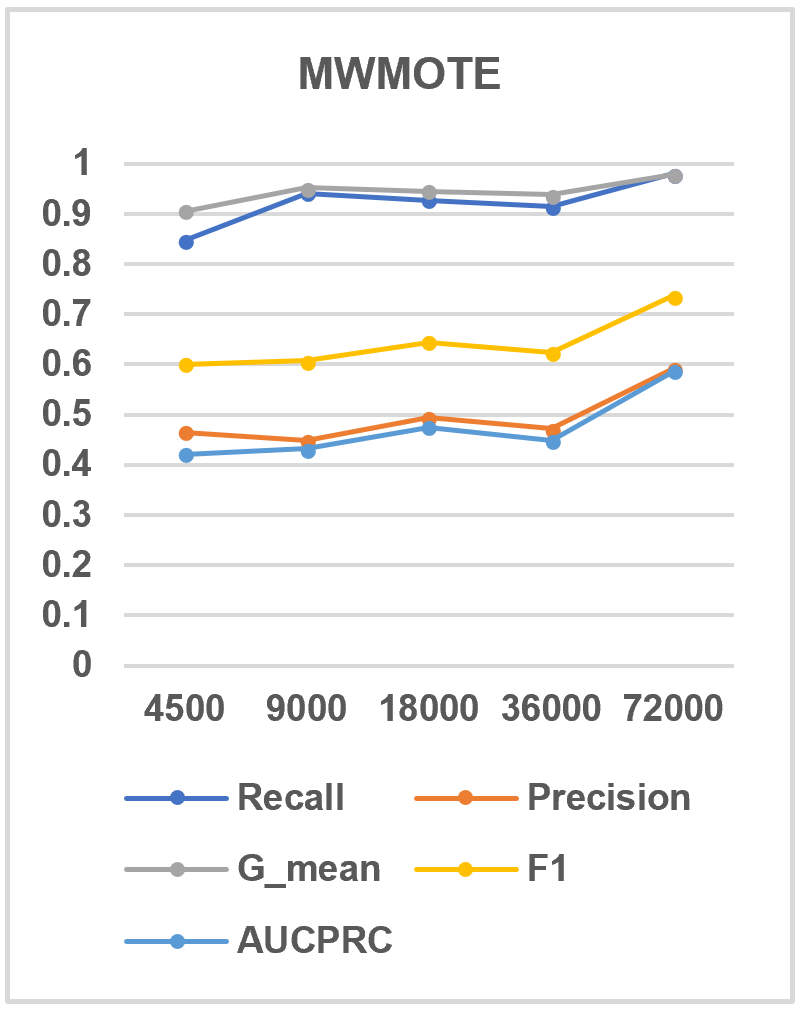
\includegraphics[width=0.8\textwidth]{images/fig26}
        \caption{MWMOTE: Impact of the Size of Dataset}
        \label{fig26}
    \end{minipage}
\end{figure}

\begin{figure}[H]
    \centering 
    \begin{minipage}{0.31\textwidth}
        \centering
        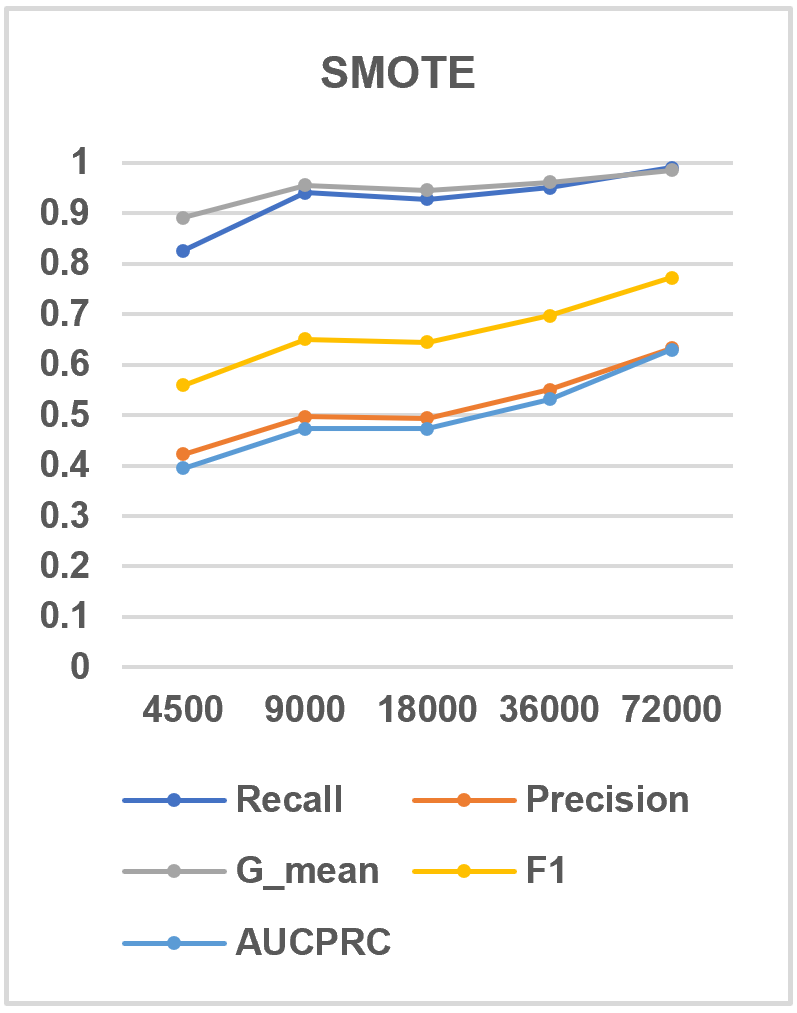
\includegraphics[width=0.8\textwidth]{images/fig27}
        \caption{SMOTE: Impact of the Size of Dataset}
        \label{fig27}
    \end{minipage}
\end{figure}

Next, in order to analyze whether the size of the dataset will affect the classification accuracy of the model, five sub-datasets with the same IR but a different number of instances (which are \#Instances=4500, 9000, 18000, 36000 and 72000) are taken from the Protein Homology dataset. The results can be observed in Figures \ref{fig18}-\ref{fig27}.

It can be seen from the figures that in the process of increasing the sample size of the algorithms DDAE, MWMOTE, SMOTE, IML and cost-sensitive Decision Tree (csDCT), the values of the five evaluation metrics have shown an upward trend, especially the precision and F1, which increases more than 0.2 and 0.1 respectively. This phenomenon shows that the classification results are more accurate on these models when the sample size is extensive compared to when the sample size is small.

The RUSBoost, AdaBoost, self-paced Ensemble Classifier and CAdaMEC algorithms are not significantly affected by the size of the dataset. The performance of the algorithms on all five experiments are quite excellent, and the value of the evaluation metrics are mostly between 0.9-1.0. Although the CAdaMEC is slightly inadequate when the total sample size is 4500, the recall value is also greater than 0.8, and as the total number of instances exceeds 10,000, this model can predict the labels of all majority and minority class correctly among all the algorithms. 

It can be noted that, only MetaCost does not show an apparent trend.

\section{Results on Effectiveness of DDAE}
\subsection{Results on Effectiveness of Components}
The DDAE model includes a total of four components, namely: Data Block Construction (DBC), Data Space Improvement (DSI), Adaptive Weight Adjustment (AWA) and Ensemble Learning (EL). In order to analyze the effectiveness of each component in the entire model, DDAE is modified by deleting the components except for EL in the model. After that, three variants are created: DDAE-DBC, DDAE-AWA and DDAE-DSI. It should be noted that since DDAE itself is an ensemble model, EL is indispensable at all times, which is why the DDAE-El is not listed in these variants. It can be observed from Figure \ref{fig27} and Figure \ref{fig28} that on two datasets (PH1 and Euthyroid Sick) when the model removes the DBC module, the recall and G-mean drops significantly, which is the poorest performance among all variants and the original model. At the same time, it can be seen that the precision varies distinctly across the variants. But the recall of DDAE without AWA or DSI does not drop as much. The performance of the original model without DSI also can be affected, which can be observed from the Figure \ref{fig27} and Figure\ref{fig28} for all evaluation metrics. Without the improvement to data space, the accuracy of prediction may decrease. All in all, the integrated algorithm of DDAE absorbs the advantages of each component so that the minority classes can be correctly classified.
\begin{figure}[h]
    \centering 
    \begin{minipage}{0.45\textwidth}
        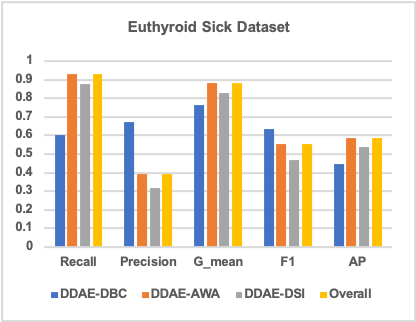
\includegraphics[width=\textwidth]{images/fig28}
        \caption{Effectiveness of DDAE on Euthyroid Sick Dataset}
        \label{fig28}
    \end{minipage}
    \quad
    \begin{minipage}{0.45\textwidth}
        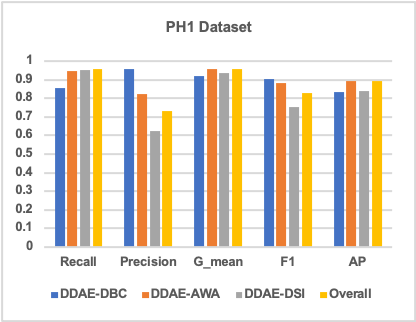
\includegraphics[width=\textwidth]{images/fig29}
        \caption{Effectiveness of DDAE on PH1 Dataset}
        \label{fig29}
    \end{minipage}
\end{figure}

\subsection{Impact of Parameters}
In this section, the impact of parameters(including the number of blocks in DBC, the relative weight between pull and push in DSI, the unstable ratio and the cost ratio in AWA) on the DDAE model is analyzed through a set of experiments. These experiments are conducted on the Cm1 and Mw1 dataset.

\begin{figure}[h]
    \centering 
    \begin{minipage}{0.45\textwidth}
        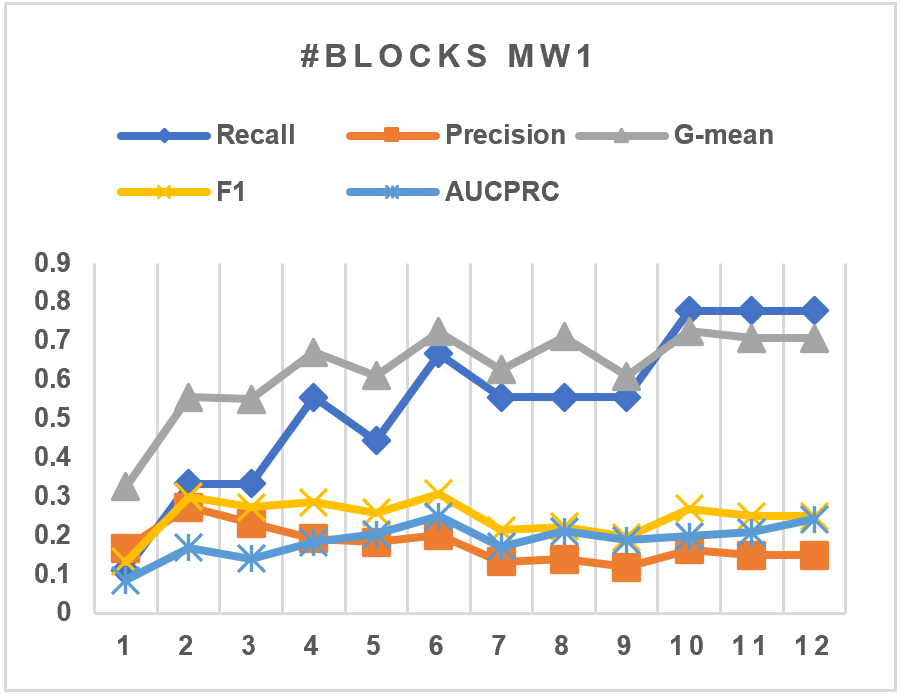
\includegraphics[width=\textwidth]{images/fig30}
        \caption{Impact of the Number of Data Blocks on Mw1}
        \label{fig30}
    \end{minipage}
    \quad
    \begin{minipage}{0.45\textwidth}
        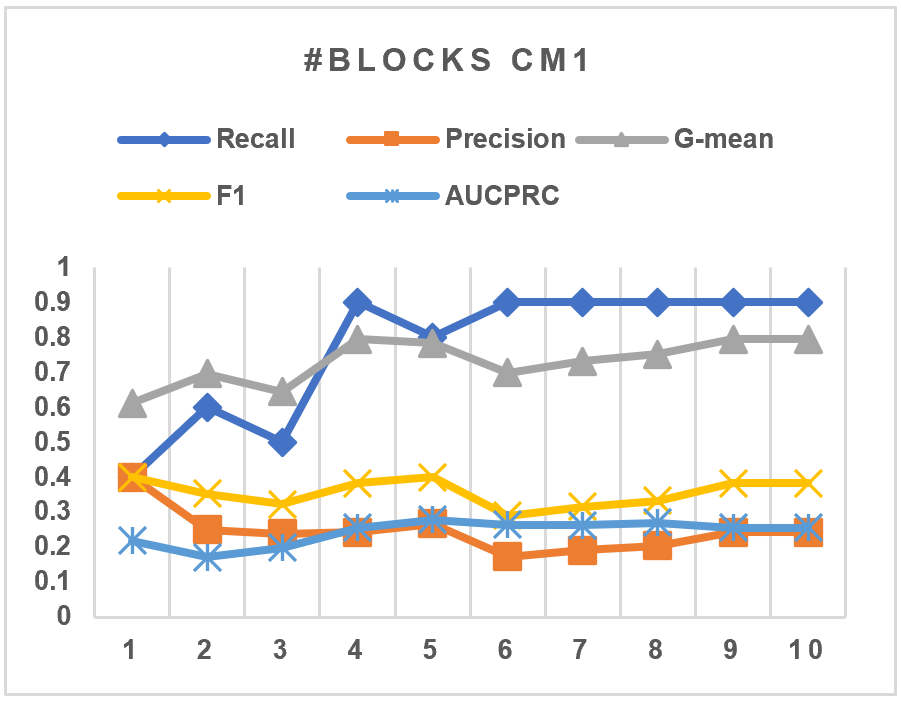
\includegraphics[width=\textwidth]{images/fig31}
        \caption{Impact of the Number of Data Blocks on Cm1}
        \label{fig31}
    \end{minipage}
\end{figure}

\subsubsection{Impact of the Number of Split Data Blocks in DBC}
The data blocks in DBC are utilized to adjust the imbalanced sample distribution so that each data block can reach a balanced level. As illustrated in Figure \ref{fig30} and Figure \ref{fig31}, a similar trend is shared among these evaluation metrics as the number of data blocks grows. It can be observed that the model works better when the number of data blocks is close to the imbalance ratio(IR(Cm1) = 10, IR(Mw1) = 12).


\subsubsection{Impact of the Relative Weight between the Pull and Push Terms in DSI}
In this section, the impact of relative weight $\omega$ between the pull and push terms in DSI is analyzed by varying $\omega$ from 0.1 to 1 on the Cm1 and Mw1 dataset. Notably, the Figure \ref{fig32} and Figure \ref{fig33} illustrate how the model achieves the best performance on Cm1 when $\omega=0.1$ and on Mw1 when $\omega=0.3$. Due to the specific data distribution on each dataset, the best choice of $\omega$ can differ.


\begin{figure}[h]
    \centering 
    \begin{minipage}{0.45\textwidth}
        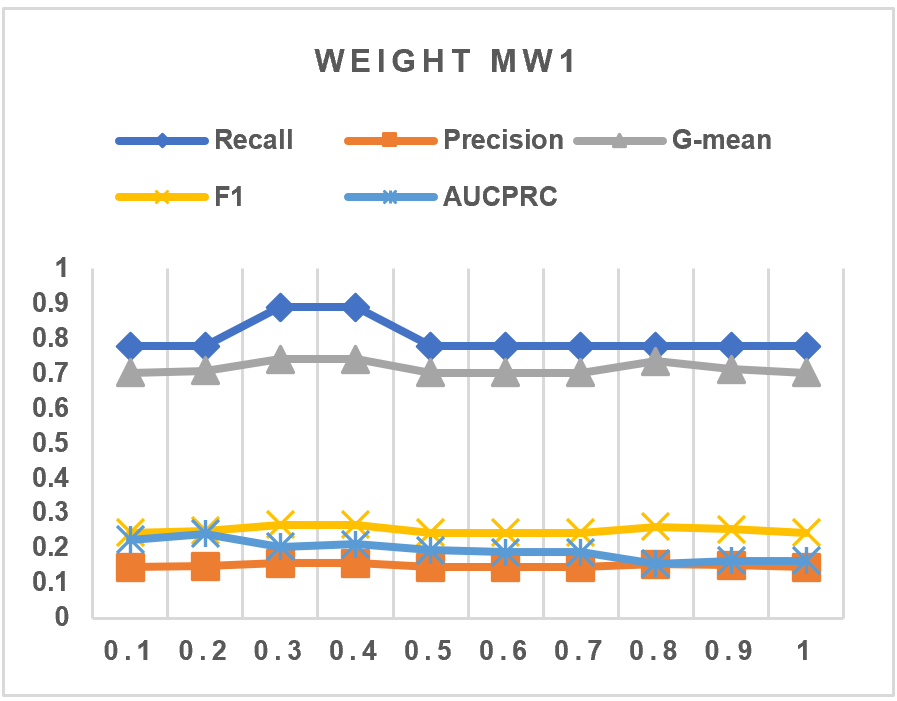
\includegraphics[width=\textwidth]{images/fig32}
        \caption{Impact of the relative Weight between the Pull and Push Terms on Mw1}
        \label{fig32}
    \end{minipage}
    \quad
    \begin{minipage}{0.45\textwidth}
        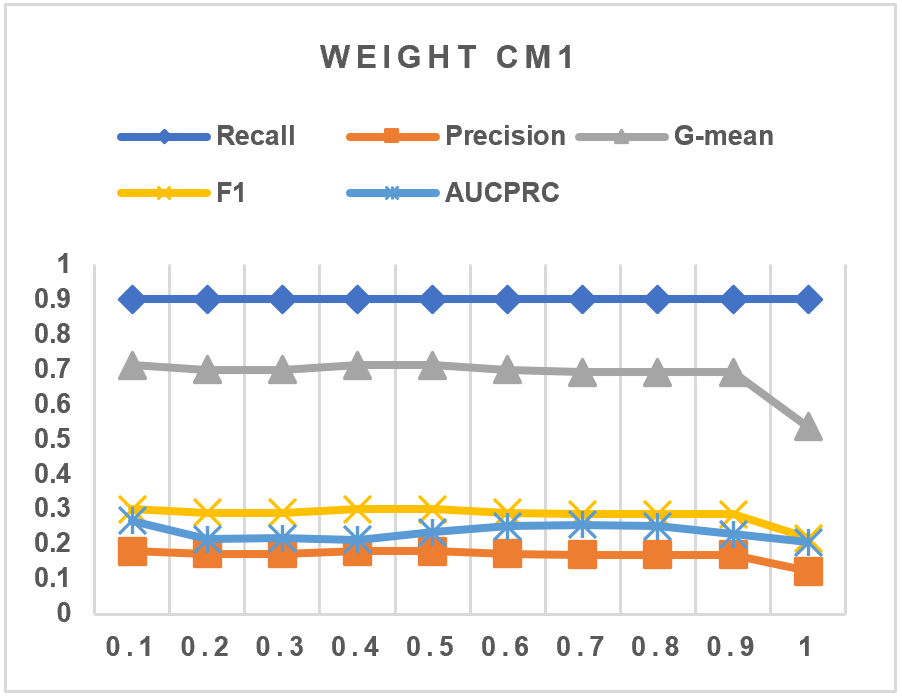
\includegraphics[width=\textwidth]{images/fig33}
        \caption{Impact of the relative Weight between the Pull and Push Terms on Cm1}
        \label{fig33}
    \end{minipage}
\end{figure}

\subsubsection{Impact of the Unstable Ratio in AWA}
% The unstable ratio $\tau$ from AWA is a threshold term that is utilized to help determine whether the AWA generated weight pair should be considered in the decision or not. In order to locate the optimal value for $\tau$, it is varied from 0.1 to 1.0 on the two given datasets. It can be observed from Figure \ref{fig35} Impact of Unstable Ratio on CM1 and Figure \ref{fig34} Impact of Unstable Ratio on MW1 obviously that, from $\tau=0.3$, the trend of these four evaluation metrics become stable and unchanged. The model achieves the best performance on Cm1 and Mw1 dataset when $\tau=0.2$ and $\tau=0.3$, respectively.
\begin{figure}[H]
    \centering 
    \begin{minipage}{0.45\textwidth}
        \includegraphics[width=\textwidth]{images/fig34}
        \caption{Impact of Unstable Ratio on Mw1}
        \label{fig34}
    \end{minipage}
    \quad
    \begin{minipage}{0.45\textwidth}
        \includegraphics[width=\textwidth]{images/fig35}
        \caption{Impact of Unstable Ratio on Cm1}
        \label{fig35}
    \end{minipage}
\end{figure}
The unstable ratio $\tau$ from AWA is a threshold term that is utilized to help determine whether the AWA generated weight pair should be considered in the decision or not. In order to locate the optimal value for $\tau$, it is varied from 0.1 to 1.0 on the two given datasets. It can be clearly observed from Figure \ref{fig34} and Figure \ref{fig35} that, from $\tau=0.3$, the trend of these four evaluation metrics becomes stable and unchanged. The model achieves the best performance on the Cm1 and Mw1 datasets when $\tau=0.2$ and $\tau=0.3$, respectively.

\subsubsection{Impact of the Cost Ratio in AWA}
\begin{figure}[H]
    \centering 
    \begin{minipage}{0.45\textwidth}
        \includegraphics[width=\textwidth]{images/fig36}
        \caption{Impact of Cost Ratio on Mw1}
        \label{fig36}
    \end{minipage}
    \quad
    \begin{minipage}{0.45\textwidth}
        \includegraphics[width=\textwidth]{images/fig37}
        \caption{Impact of Cost Ratio on Cm1}
        \label{fig37}
    \end{minipage}
\end{figure}

As introduced in Chapter 2, the most significant step of the cost-sensitive learning method is choosing the cost for False Positive (FP) and False Negative (FN), and the cost ratio shows which class is more important in the classification process. But if there is no experts' suggestions or any other additional information related to these two classes, the decision of an appropriate cost ratio may become difficult. In this experiment, the tested range of cost ratio is from 1 to the imbalance ratio. For instance, cost ratio = 1 means the two classes are equally important. From Figure \ref{fig36} and Figure \ref{fig37}, it can be seen that, when the cost ratio is above 2, the performance of the model remains stable on both datasets. 
    %\myemptypage

    \chapter{Discussion and Conclusion}
The objective of this paper was to compare the performance of various class imbalance classification models when dealing with imbalanced medical/healthcare datasets. For this, DDAE, MWMOTE, SMOTE, RUSBoost, AdaBoost, cost-sensitive decision tree (csDCT), MetaCost, CAdaMEC, self-paced Ensemble Classifier and Iterative Metric Learning (IML) were utilized to classify some testing samples from various imbalanced medical/healthcare datasets. All the imbalanced datasets came from UCI, KEEL and OpenML with different imbalance ratios (IR). The experiments were divided into two stages. In the first stage, each model was used to deal with each given dataset. In addition, a further two experiments focused on the impact of various imbalance ratios and the size of datasets on the performance of models. The second stage focused on the impact of parameters on the DDAE model and the effectiveness of its different components. 

The results of the experiments carried out for this paper are reported in Chapter 4. This section contains the overall discussion of the results and influencing factors of these models.

DDAE yielded the highest value for recall on almost all imbalanced datasets, not only on medical/healthcare data but also on datasets from other sectors. Since the recall only focuses on minority, a higher recall means that most samples with a class label of 1 can be correctly predicted. In the medical or healthcare sector, successfully detecting as many people in genuine need of medical intervention can be the most critical goal. However, this does not mean that recall is the most significant evaluation metric when the classifier is used on medical datasets. For example, if DDAE is used to test whether a person has infected by Corona Virus, even though all the infected cases can be screened out (meaning recall is 1), a low precision means that, compared with actual patients, several times more healthy people will be incorrectly diagnosed as infected. This is undesirable at this stage, and may even cause social catastrophe. According to the description of PRC, it can be seen that the recall and precision cannot be satisfactory at the same time, so it is critical for a class imbalance classification model to achieve an appropriate F1. Comparing with other algorithms like csDCT, RUSBoost and self-paced Ensemble Classifier, the F1 of DDAE is extremely low on some datasets. This illustrates that DDAE is more sensitive than others, so it is easier to predict a sample with a class label of 0 as 1, which can be considered first because the number of training samples is too small. On several datasets, such as Poker8vs6, DDAE's F1 performs extremely poorly compared to other algorithms but has better recall performance. This dataset contains a total of 1,477 samples, but its IR is as high as 85.882, that is, only 17 positive samples are included in this dataset. According to the description of DDAE in Chapter 3, the whole training set was divided into 79 data blocks to train each base classifier with each block only consisting of 26 samples (13 positive samples and 13 negative samples). Although each data block reaches a balanced state, when the total number of samples is small and the degree of imbalance is high, the sub-training set obtained by resampling is incomplete. This may cause the model to overfit to minority, fail to learn more robust and easy generalization features, and often have worse generalization performance on highly skewed data. Under these circumstances, if AWA in DDAE assign a non-default weight to minority, the model will become more sensitive to the minority class, which will cause a low precision. Comparing to Poker8vs6, the performance of F1 on PH1 (with 11,274 data samples) and optdigits (with 5,620 data samples) is much better. This can also be confirmed from Figure \ref{fig17} and Figure \ref{fig16}, which shows that when the size of dataset is constant, as the IR increases, the F1 and AUCPRC of DDAE on individual dataset shows a significant decrease.

Iterative Metric Learning (IML) is a model that also utilizes Large Margin Nearest Neighbor (LMNN) to improve the data space and uses the kNN classifier as the basic classifier. Unlike DDAE, IML always performs well in F1 and AUCPRC, even though the value of recall is low. It can be observed that the evaluation metrics of IML on different datasets varies, meaning that compared with other models, IML is more sensitive to the data distribution of the dataset. From the results in section 4.2.2, it can be observed that, even the IR climbs up, while the evaluation metrics of IML keep stable.

The performance of SMOTE and MWMOTE are similar to some extent, but it is evident that the value of G-mean, F1 and AUCPRC for SMOTE on some slightly imbalanced datasets, such as WDBC (IR=1.866) and PID (IR=1.684), is better than that of MWMOTE. This can also be observed from Figure \ref{fig17}, which shows that the IR is relatively small, SMOTE can achieve a better performance than MWMOTE. SMOTE will randomly select minority samples to synthesize new samples, regardless of the surrounding samples. This may cause the generation of useless samples if the selected minority sample is far away from the decision boundary or the newly generated samples may be overlapped with the majority samples in the surrounding if the selected minority reside inside the majority area \cite{61}. MWMOTE also applies the synthetic sample generation technique. However, unlike SMOTE, MWMOTE utilizes a clustering procedure to ensure that all the produced samples must be located within the minority region to avoid any false or noisy synthetic samples \cite{62}. MWMOTE also finds a more practical approach to select samples that are difficult to learn, and then an appropriate weight will be assigned to them \cite{62}, which SMOTE does not consider. This can explain why MWMOTE performs better than SMOTE under circumstances where the IR is high. 

RUSBoost, AdaBoost and self-paced Ensemble Classifier are three alternative ensemble learning techniques to DDAE. It should be noted that the performance of RUSBoost and AdaBoost is very similar. Compared with RUSBoost, the self-paced Ensemble Classifier and AdaBoost show a more stable performance. Even though RUSBoost and AdaBoost achieve 0.214 and 0.196  respectively in terms of recall on the Pc3 dataset, the recall of the self-paced Ensemble Classifier is 0.786 for this dataset, which yielding the highest value among all models compared. AdaBoost is a basic implementation of the ensemble learning technique. RUSBoost adds a random undersampling technique on the foundation of boosting. Like DDAE, the self-paced Ensemble Classifier also cuts the majority of the dataset into several bins and uses the resampled balance training set (including majority subset and minority subset) to train each base classifier. The self-paced Ensemble Classifier, RUSBoost and AdaBoost, when compared with DDAE, do not take the weight of both classes into concern, which can also contribute to a lower recall value but higher F1 and AUCPRC values. 

Moreover, the remaining of the algorithms are all implementations of cost-sensitive learning, namely MetaCost, csDCT and CAdaMEC. It can be observed that these models can perform well when the IR of the dataset is relatively low, such as in the Euthyroid Sick, optdigits and PH1 datasets. The performance of MetaCost varies when it deals with different datasets. It is hard to set an appropriate cost matrix for each dataset, as people cannot be experts all the time. If the set cost matrix is not suitable for the predicted dataset and the data is highly skewed, the performance of the classifier can be extremely unsatisfactory, such as on the Poker8vs6 dataset. Considering this, it is better to utilize this kind of classifier when the imbalance ratio is not very high. This was also confirmed through the experiments in section 4.2.2, which showed that as the imbalance ratio increases, the curves of all evaluation metrics of MetaCost and CAdaMEC fluctuate, but still show a downward trend.

% It is clear that many models can maintain a high value in terms of recall and G-mean even though the imbalance ratio is great, which means a large proportion of minorities and majorities can be correctly screened out. If the recall stays almost stable or has a slight decrease as the imbalance ratio increase, it can be observed that the precision of this model must show a downward trend, such as in DDAE, csDCT, MWMOTE, SMOTE. This shows that as the data distribution becomes more and more imbalanced, these models may overfit to minority. Since the F1 and AUCPRC take both recall and precision into account, these two metrics also show a downward trend. IML and MetaCost show less relationship with the changes in imbalance ratio. The former has an almost stable performance, and the latter shows an irregular fluctuation during this process. When considering F1 and AUCPRC, AdaBoost and RUSBoost perform better when the imbalance ratio is higher than 30.

The impact of the size of the dataset on the performance of the model is noticeable. Except for Metacost, which dispalys an irregular fluctuation, the remaining algorithms either continue to perform very well or all the evaluation metrics of the algorithm rise gradually as the number of samples in the dataset increases. For most algorithms, the more samples in the dataset, the more training samples are used to train the model, which can provide a stronger training basis for the model and enable more accurate prediction. Enlarging the scale of the dataset can enhance the completeness of the data, and can also alleviate the over-fitting phenomenon caused by the resampling method, such as in MWMOTE and SMOTE.

From section 4.3.1, it can be seen that the recall and G-mean drop significantly when the DBC component has been removed. The variant DDAE-DBC displays the poorest performance among all other variants and the original model. This phenomenon shows that DBC plays a vital role in the process of identifying minority samples. DBC turns the data distribution of each data block into a nearly balanced state, which leads to the improvement of the minority’s ‘status’ so that the model can classify minority samples correctly. However, this component has also cause the problem of overfitting, since the removal of DBC lead to a significant decrease on recall but increase on precision. DBC is also critical because it provides support for AWA and EL components. Due to the different data distribution, AWA components may be ‘abandoned’ sometimes( which means the default weight pair is assigned to the model), but it does not mean AWA is dispensable. On the PH1 dataset, the recall and G-mean of DDAE-AWA perform less satisfactory than the original model. Considering all these evaluation metrics, the original model should be used under some specific circumstances, for instance, when the misclassifcation of majority samples can be ignored.

Given the importance of the DBC component, the selection of an appropriate number of data blocks is also a critical problem. According to the previous description of DBC in Chapter 3, when the original dataset is divided into a small number of blocks, the data distribution in every single block can still maintain imbalance. Thus, it can be seen that DDAE achieves increased performance when the number of data blocks is close to the imbalance ratio value. Nevertheless, the imbalance ratio is not the only option. Notably, the model can also reach a promising performance when the number of data blocks is 4 and 9 on the Cm1 and 10 and 11 on the Mw1 dataset. This phenomenon illustrates that the original dataset might be divided into a smaller number of blocks instead of the value of IR blocks. From this experiment, it can be seen that the number of base estimators set by ensemble learning algorithms also has an impact on the algorithm performance.

When should the two different classes be pushed away from each other, and when should the same class be pulled closer to each other? The answer to this question may lead to the decision of the relative weight $\omega$ between pull and push term in the DSI component. For instance, when the data instances from these two classes overlap to a high degree, it is best to push them away from each other through setting a considerable value of $\omega$. On the contrary, if an area is occupied by the majority class instances, it may be critical to set a smaller value at $\omega$ in order to bring the minority instances with the same label closer together. 
The adoption of the AWA component is decided by a threshold $\tau$ called unstable ratio. According to the result in this section, the best $\tau$ should be set to 0.2.

In AWA, the cost ratio represents the importance of the costs between the majority and minority classes. To be specific, when the cost ratio is set to 1, the majority class and minority class have an equal ‘status’, as if both of them, are the king of their kingdom. However, from the results presented in this section, all the metrics become stable when the cost ratio is greater than two on both of the datasets in the experiment, showing that the different selection of cost ratio does not affect the performance of the model. This shows the data sources do not restrict the DDAE. The overall results in section 4.1.1 also confirm that even when the datasets are from different fields, the DDAE can deal with them well. This matches the finding stated in study \cite{73}.

In this paper, all the experiments focused on the binary classification. However, some of the algorithms used for comparison are also suitable for multi-class classification, such as AdaBoost, MetaCost, cost-sensitive decision tree. SMOTE, MWMOTE and IML focuses on the feature space. Thus, if these techniques are utilized for multi-class classification, the classifier combined with these techniques should be suitable for multi-class classification.

\begin{table}[]
    %\centering
    % \tiny
    \begin{tabular}{|p{0.18\textwidth}<{\centering}|p{0.25\textwidth}|p{0.3\textwidth}|p{0.18\textwidth}|}
    \hline
    \textbf{Technique}        & \textbf{Pros} & \textbf{Cons} & \textbf{Example} \\ \hline
    \textbf{Oversampling} 
    & Balance the class distribution of original dataset                
    & Depend on the distribution of minority samples;\newline Require a lot of additional computing resources;\newline May cause the problem of overfitting
    & SMOTE\newline MWMOTE\newline DDAE\\ \hline
    \textbf{Undersampling}   
    & Balance the class distribution of original dataset                
    & May cause the information loss and the problem of underfitting                
    &RUSBoost\newline DDAE       \\ \hline
    \textbf{Cost-sensitive Learning}            
    & Take the importance of different class into account                
    & Hard to set an appropriate cost matrix for each dataset            & MetaCost\newline CAdaMEC\newline csDCT\newline DDAE  \\ \hline
    \textbf{Ensemble Learning}            
    & Stable;\newline Make more reliable predictions than the single classifier;\newline Reduce the dispersion of model performance                
    & Absorb not only the advantages but also the disadvantages of used techniques when the final classifier is combined with several techniques       
    & RUSBoost\newline AdaBoost\newline self-paced Ensemble Classifier\newline DDAE  \\ \hline
    \textbf{Distance Metric Learning}            
    & Result in a stable neighborhood for each sample                
    & Depend on the data distribution in the feature space, when the dataset is highly imbalance with a relatively small size, the performance can be unsatisfactory               
    &IML\newline DDAE        \\ \hline
    \end{tabular}
    \caption{Pros and Cons of different Techniques utilized for dealing with Class Imbalance Problem}
    \label{tab26}
\end{table}

In summary, this paper investigated the performance comparison of several class imbalance classification models using medical/healthcare datasets and also some datasets from other fields.  Table \ref{tab26} shows the characteristics of techniques used for dealing with class imbalance problem. Since algorithms have various characteristics, it is important to choose the appropriate algorithm depending on the actual situation. For instance, for the algorithms used for stocks prediction, people should pay more attention to their predictions. However, in medical diagnosis or earthquake prediction sector, the recall for the algorithms is more significant. The performance of algorithms cannot be judged by the individual evaluation metric, the actual request and situation should also be taken into account.
% The algorithm that uses undersampling inevitably discards most of the majority samples when the imbalance ratio is high, causing information loss, while the algorithms that uses the oversampling method generates huge amounts of data when the amount of data is large and the imbalance ratio is high, which requires a lot of additional computing resources. Oversampling, such as SMOTE and MWMOTE, is based on the distribution of the minority class samples. When the “quality” of the minority class is poor, this method may be worse than direct training. For cost-sensitive learning methods, such as MetaCost, csDCT and CAdaMEC, it is hard to set an appropriate cost matrix for each dataset as people cannot be experts all the time. If the set cost matrix is not suitable for the to be predicted dataset, the performance of the classifier can be unsatisfactory. Therefore, it is better to utilize this kind of classifier when the imbalance ratio is not very high. Considering ensemble learning methods, its performance can be satisfactory most of the time, but this study identified that due to the ensemble process the final classifier can absorb not only the advantages but also the disadvantages of used techniques. 
In addition, the number of base estimators set by ensemble learning classifiers can also make an impact on their performance. This has already been researched with regard to DDAE, but more detail surrounding the impact of the number of base estimators on other ensemble classifiers remains an area for the future research.

    %\myemptypage

    % \chapter{Conclusion}
In this chapter, the conclusion of ...

    % \myemptypage

    %--- references ---
    \bibliographystyle{IEEEtran}
    \bibliography{content/references}
    \addcontentsline{toc}{chapter}{\bibname}
    %\myemptypage

    %--- appendix ---
    \begin{appendix}
        \input{content/appendix_a}
        \myemptypage
    \end{appendix}
    
\end{document}